\documentclass[12pt]{article}
\usepackage{amsmath, amssymb, amsthm, tikz}
\usetikzlibrary{decorations.pathmorphing}
\usepackage{color}

%\pagecolor{black}
%\color{white}

\addtolength{\textwidth}{2.5in}
\addtolength{\hoffset}{-1.25in}
\addtolength{\textheight}{2.0in}
\addtolength{\voffset}{-1.0in}

\usepackage{bbm}


\newcommand{\op}[1]  { \operatorname{ #1 }}
\newcommand{\logG} {\operatorname {log \Gamma}}
\newcommand{\olbbH}[0]  { \overline{\mathbb{H}}}
\newcommand{\olbbQ}[0]  { \overline{\mathbb{Q}}}
\newcommand{\olG}[0]  { \overline{\Gamma}}
\newcommand{\bbH}[0]  { \mathbb{H}}
\newcommand{\bbC}[0]  { \mathbb{C}}
\newcommand{\bbZ}[0]  { \mathbb{Z}}
\newcommand{\bbQ}[0]  { \mathbb{Q}}
\newcommand{\bbR}[0]  { \mathbb{R}}
\newcommand{\gok}[0]  { \mathfrak{k}}
\newcommand{\goe}[0]  { \mathfrak{e}}

\newcommand{\ee}[0] {\mathbbm{e}}
\newcommand{\ii}[0] {\mathbbm{i}}
\newcommand{\dd}[0] {\mathbbm{d}}
%\newcommand{\ee}[0] {e}
%\newcommand{\ii}[0] {i}


\numberwithin{equation}{section}
\newtheorem{theorem}{Theorem}[section]
\newtheorem{definition}[theorem]{Definition}
\newtheorem{lemma}[theorem]{Lemma}
\newtheorem{remark}[theorem]{Remark}
\newtheorem{entry}[theorem]{Entry}
\newtheorem{corollary}[theorem]{Corollary}
\newtheorem{proposition}[theorem]{Proposition}
\newtheorem{example}[theorem]{Example}
%\mathtoolsset{showonlyrefs=true}


\newcommand{\Head}[3] {{}_{#1}{#2}_{#3}}
\newcommand{\Arg}[3] {\left( \begin{array}{c} #1 \\ #2 \end{array} \Big| {#3}  \right)}
\newcommand{\ArgS}[3] {( \begin{smallmatrix} #1 \\ #2 \end{smallmatrix} | {#3})} 

\newcommand{\ArgKS}[1] {\ArgS{\frac12,\frac12}{1}{#1}}

\newcommand{\FF}[6] {{}_{#1}{#2}_{#3} \left( \begin{array}{c} #4 \\ #5 \end{array} \Big| {#6}  \right)}
\newcommand{\FFs}[6] {{}_{#1}{#2}_{#3} ( \begin{smallmatrix} #4 \\ #5 \end{smallmatrix} | {#6}  )}
\newcommand{\FFe}[7] {{}_{#1}^{\,}{#2}_{#3}^{#4} \left( \begin{array}{c} #5 \\ #6 \end{array} \Big| {#7} \right)}
\newcommand{\FFes}[7] {{}_{#1}^{\,}{#2}_{#3}^{#4} ( \begin{smallmatrix} #5 \\ #6 \end{smallmatrix} | {#7} )}
\newcommand{\FFf}[5] {{}_{#1}{#2}_{#3} \left(#4 | {#5} \right)}
\newcommand{\FFef}[6] {{}_{#1}^{\,}{#2}_{#3}^{#4} \left(#5 | {#6} \right)}

\newcommand{\ARG}[2] {\left( \begin{array}{c} #1 \\ #2 \end{array} \right)}

\newcommand{\bfa}[0] {\mathbf{a}}
\newcommand{\bfb}[0] {\mathbf{b}}
\newcommand{\bfm}[0] {\mathbf{m}}
\newcommand{\bfn}[0] {\mathbf{n}}
\newcommand{\bfx}[0] {\mathbf{x}}
\newcommand{\bfy}[0] {\mathbf{y}}

\author{}
\title{Calculating $\, _{p}F_{q}$}
\date{}

\begin{document}
\maketitle

\abstract{The generalized hypergeometric function $\FFf{p}{F}{q}{\bfa; \bfb}{z}$ is susceptible to various numerical evaluation techniques. Here we attempt to give effective strategies for unrestricted $z$ while restricting the parameters so that $||\bfa||+||\bfb||$ does not exceed the roughly the working bit precision. The problem of large parameters is \emph{not} considered, and the techiniques considered are rigorous, that is, they produce a proven enclosure of the value of the function.}

\section{Definitions}
For $\mathbf{a}=a_1,\dots,a_p$ and  $\mathbf{b}=b_1,\dots,b_q$, set $(a)_n := \Gamma(a+n)/\Gamma(a)$ and $(\mathbf{a})_n := \prod_i (a_i)_n$ and define
\begin{equation}
\label{Fdef}
\FF{p}{F}{q}{\mathbf{a}}{\mathbf{b}}{z} := \sum_{n=0}^{\infty} \frac{(\mathbf{a})_n}{(\mathbf{b})_n} \frac{z^n}{n!}
\end{equation}
The function is undefined when any $b_i$ is $0,-1,-2,\dots$, i.e. $\Gamma(\mathbf{b}) := \prod_i \Gamma(b_i)$ is infinite. When either $z$ or $1/\Gamma(\bfa)$ is zero, the series terminates and \eqref{Fdef} provides a perfectly reasonable definition in this case.

Since the difference in parameter counts $q+1-p$ controls the most important properties of these functions, set $d=q+1-p$ for any $p$ and $q$. The series \eqref{Fdef} defines an entire function of $z$ for $d > 0$ and diverges for $d<0$. For $d<2$, the hypergeometric function can be defined in the non-terminating case on a section of the Riemann surface of $\log(-z)$ by
\begin{equation}
\label{mbint}
\FF{p}{F}{q}{\mathbf{a}}{\mathbf{b}}{z} = \frac{\Gamma(\mathbf{b})}{\Gamma(\mathbf{a})} \int_{-\ii \infty}^{+\ii \infty} \frac{\Gamma(\mathbf{a}+s) \Gamma(-s)}{\Gamma(\mathbf{b}+s)} (-z)^s \frac{ds}{2\pi \ii}\text{,} \quad |\arg(-z)| < (2-d) \tfrac{\pi}{2}\text{.}
\end{equation}
When $d=0$ the branch structure is even richer due to a singularity at $z=1$ and the Riemann surface of $\log$ is no longer sufficient to describe a branch. The integer $d$ can also be viewed as a measure of the difficulty in evaluating the function: $d=0$ can be handled by various connection formulas with convergent series, and the function poses more difficulties as $d$ moves away from $0$ due to increasingly more difficult essential singularities. The standard quantity
$\sigma = \Sigma(\mathbf{b}) - \Sigma(\mathbf{a})$ is also relevent when $d \ge 0$.

Since functions accept numbers and not points on Riemann surfaces, we will use ${}_p F_{q} = {}_p F_{q}^{+}$ to denote the usual branch with continuity from below $\mathbb{R}_{+}$ and ${}_p^{\,} F_{q}^{-}$ for the non-standard continuity from above $\mathbb{R}_{+}$. For example, $\Head{1}{F}{0}^{-}(a|z) = (-1/z)^a (1-1/z)^{-a}$ and $\FFs{2}{F}{1}{a,b}{c}{z} = (1-z)^{-a} \FFes{2}{F}{1}{-}{a,c-b}{c}{\tfrac{z}{z-1}}$. Whenever a possibly infinite quantity $\Gamma(a_i-a_j)$ appears in a formula \footnote{that is, when the list $\bfa$ has duplicates modulo $\mathbb{Z}$} that formula should be interpreted via a limiting case of the general formula. Also, $\hat{\mathbf{a}}_i$ denotes the length $p-1$ vector with the $i^{\text{th}}$ entry omitted.

The imaginary unit is denoted by $\ii = \sqrt{-1}$, and $\ee = 2.718\dots$ is Euler's number.

\section{The case $d=0$}
Here we have several usual transcendental functions, rational possibilities, and algebraic possibilities.
\begin{align*}
\FF{3}{F}{2}{1,2,3}{4,5}{z} &= \frac{36}{z^3}+\frac{90}{z^2}-\frac{6}{z}+\left
   (\frac{36}{z^4}-\frac{36}{z^2}\right) \log
   (1-z)-\frac{72}{z^3}
   \text{Li}_2(z)\text{,}\\
\FF{3}{F}{2}{5,4,3}{2,1}{z} &= \frac{140}{(1-z)^9}-\frac{315}{(1-z)^8}+\frac{240}{(1-z)^7}-\frac{70}{(1-z)^6}+\frac{6}{(1-z)^5}\text{,}\\
\FFf{2}{F}{1}{-\tfrac{1}{6}, \tfrac{1}{6};\tfrac{1}{2}}{z} &= \tfrac{1}{2} \left(\sqrt{1-z}+\sqrt{-z}\right)^{1/3}+\tfrac{1}{2} \left(\sqrt{1-z}-\sqrt{-z}\right)^{1/3}\text{.}
\end{align*}
In general ${}_{p}F_{p-1}(z)$ has singularities at $z=1$ and $z=\infty$ with a standard branch cut along the real axis $[1,\infty]$. For agreement with the usual transcendental functions, the standard value on the branch cut is determined by continuity from below.

\subsection{inside unit circle}
For arguments sufficiently inside the unit circle, we can just sum the series. Besides the implementation details of how to actually sum the series, there is not much else to say here.

\subsection{outside unit circle}
The residues on the left of \eqref{mbint} give
\begin{equation}
\label{balanced_outside}
\FF{p}{F}{p-1}{\mathbf{a}}{\mathbf{b}}{z} = \sum_{i=1}^{p} \frac{\Gamma(\mathbf{b}) \Gamma(\hat{\mathbf{a}}_i-a_i)}{\Gamma(\mathbf{b}-a_i) \Gamma(\hat{\mathbf{a}}_i)} (-z)^{-a_i} \FFe{p}{F}{p-1}{-}{a_i,1+a_i-\mathbf{b}}{1+a_i-\hat{\mathbf{a}}_i}{\frac{1}{z}}
\end{equation}
and for arguments sufficiently outside the unit circle we can just sum the series on the right.

\subsection{near unit circle, away from one}
The hypergeometric function can be evaluated non-rigorously near the the unit circle using various sequence transformations or Pad\'e approximations. The series may be evaluated rigorously via a convergent series for any $z \not \in [1,\infty]$ by the right hand side of
\begin{equation}
\label{balanced_anywhere}
\FF{p}{F}{p-1}{\mathbf{a}}{\mathbf{b}}{z} = (\tfrac12+ \tfrac12 \sqrt{1-z})^{-2 a_p} \sum_{n=0}^{\infty}u_n \left(\frac{1-\sqrt{1-z}}{1+\sqrt{1-z}}\right)^n
\end{equation}
However, since computation of the $u_n$s is a bit expensive, it should only be used when absolutely neccessary. Furthermore, the convergence rate is only acceptable sufficiently far away from the branch cut $[1,\infty]$. The algebraic prefactor is not strictly necessary but there is good reason for it. It is present in many quadratic transformation formulas in special cases and has the effect of lowering the order of the recurrence relation for $u_n$ from $2p-1$ to $2p-2$.

For $\Head{2}{F}{1}$, Fateman cites Gosper giving $f_k \to \Head{2}{F}{1}(a,b;c|z)$ (but no error bound) with 
\begin{equation*}
\begin{aligned}
d_0 = 0\text{,} \quad d_{k+1} & = \tfrac{(k+a)(k+b)z}{(k+1)(2k+c)(2k+c+1)}(e_k-(k+c-b-a)\tfrac{z}{1-z} d_k)\\
e_0 =1\text{,} \quad e_{k+1} & = \tfrac{(k+a)(k+b)z}{(k+1)(2k+c)(2k+c+1)}(\tfrac{a b z}{1-z} d_k+(k+c) e_k)\\
f_0 = 0\text{,} \quad f_{k+1} &= f_{k} + e_k - \tfrac{k((k+c-b-a)z-(2k+c))-a b z}{(2k+c)(1-z)} d_k
\end{aligned}
\end{equation*}
However, \eqref{balanced_anywhere} is not much different as the $u_n$ (with $a_p:=a$) satisfy $u_0 = 1$, $u_1 = \frac{4ab}{c}-2a$ and
\begin{equation*}
u_{n+1} = \tfrac{2(2b-c)(n+a)}{(n+1)(n+c)} u_n + (1-\tfrac{2(1-2a+c)(n+a)}{(n+1)(n+c)}) u_{n-1}\text{.}
\end{equation*}

\begin{theorem}
Gosper's $f_k \to \Head{2}{F}{1}(a,b;c|z)$ is correct for $|\frac{z^2}{4(z-1)}|<1$.
\end{theorem}
\begin{remark}
The convergence criterion and iteration should be compared with Theorem \ref{thm_4e3_2e1_2e1}.
\end{remark}
\begin{proof}(sketch)
Maybe start with
\begin{equation*}
\begin{pmatrix}
\Head{2}{F}{1} \ArgS{a,b}{c}{z} \\ z \frac{\partial}{\partial z} \Head{2}{F}{1}\ArgS{a,b}{c}{z}
\end{pmatrix}
 = \sum_{n=0}^{\infty}
\prod_{k=0}^{n-1}
\tfrac{(k+a)(k+b)z}{(k+1)(k+c)}
\begin{pmatrix}
1 & 0 \\
k+1 & 0
\end{pmatrix}
\cdot \begin{pmatrix}
1 \\
0
\end{pmatrix}\text{,}
\end{equation*}
...
adapt Gosper's ``Acceleration of Series'' to matrices
...
This should give
\begin{equation*}
\begin{pmatrix}
\Head{2}{F}{1} \ArgS{a,b}{c}{z} \\ z \frac{\partial}{\partial z} \Head{2}{F}{1}\ArgS{a,b}{c}{z}
\end{pmatrix}
 = \sum_{n=0}^{\infty}
\prod_{k=0}^{n-1}
\tfrac{(k+a)(k+b)z}{(k+1)(2k+c)(2k+c+1)}
\begin{pmatrix}
k+c & 1 \\
\frac{a b z}{1-z} & \frac{(k+c-a-b)z}{z-1}
\end{pmatrix}
\cdot \begin{pmatrix}
1 \\
\tfrac{n((n+c-b-a)z-(2n+c))-a b z}{(2n+c)(z-1)}
\end{pmatrix}\text{,}
\end{equation*}
and also shows that starting with $d_0=1, e_0=0$ results in $f_k \to z \frac{\partial}{\partial z} \Head{2}{F}{1}(a,b;c|z)$.
\end{proof}

\subsection{near one}
This is the most interesting case as the function can fail to be defined at one. The existence of $F(1)$ is determined by $\Re(\sigma)> 0$. If $\sigma$ is not an integer we have
\begin{equation}
\label{nearone}
\FF{p}{F}{p-1}{\mathbf{a}}{\mathbf{b}}{1-z} = \sum_{n=0}^{\infty} u_n \left(\begin{array}{c} \mathbf{a}\\\mathbf{b}\end{array} \right) z^{\sigma+n} + \sum_{n=0}^{\infty} v_n \left(\begin{array}{c} \mathbf{a}\\\mathbf{b}\end{array} \right) z^n
\end{equation}
with the $u_1,u_2,\dots$ determined from a recurrence by $u_0 = \Gamma(-\sigma)\Gamma(\mathbf{b})/\Gamma(\mathbf{a})$ and the $v_{p-1}, v_p, \dots$ are determined from a recurrence of order $p-1$ by $v_0, \dots, v_{p-2}$. Thus, the difficulty is computing these $v_0, \dots, v_{p-2}$. Gauss derived $v_0 = \Gamma(\sigma)\Gamma(b_1)/\Gamma(b_1-\bfa)$ when $p=2$.

If $\sigma$ is an integer, then at most one $\log(z)$ enters into the series.

\subsubsection{generic approach}
We simply evaluate Equation \eqref{nearone} and its derivatives up to and including order $p-1$ at $z=1/4$ to solve for the $u_0,v_0,\dots,v_{p-2}$. The explicit formula for $u_0$ is surprisingly useless in this approach.

\subsubsection{Buehring}
Here we sum the first $m$ terms of Equation \eqref{Fdef} and use a formula derived by Buehring to sum the remaining terms. Since we will be dealing with logarithmically convergent series (when $z=1$) in both sums, it is important to balance the choice of $m$ between the two to ensure a sub-exponential algorithm. The basic idea is that although the convergence of the series $\Sigma_n n^{-m}$ is ultimately slow (logarithmic), if $m$ is large enough relative to the target precision, the ``slow'' part of the sum is never reached.

We have (Equations (2.7) and (2.9) in ``analytic continuation of the generalized hypergeoemtric series near unit argument with emphasis on the zero-balanced series'' by Buehring and Srivastava)
\begin{align}
\nonumber
\sum_{n=m}^{\infty}{\frac{(\mathbf{a})_n}{(\mathbf{b})_n} \frac{z^n}{n!}}&=\frac{\Gamma(\mathbf{b})}{\Gamma(\mathbf{a})} z^m \sum_{k=0}^{\infty} {\frac{\Gamma(\mathbf{a}+m+k)}{\Gamma(\mathbf{b}+m+k)} \frac{z^k}{\Gamma(1+m+k)}}\\
\label{buehring}
&=\frac{\Gamma(\mathbf{b})(a_p)_m}{\Gamma(\hat{\mathbf{a}}_p)} z^m \sum_{k=0}^{\infty} {A_k\left(\begin{array}{c} \hat{\mathbf{a}}_p \\ \mathbf{b} \end{array}\right)} \,{} _2\tilde{F}_1\left( \begin{array}{c} 1,a_p+m \\ 1+\sigma+a_p+m+k \end{array} \Big| z\right)
\end{align}
where the $A_k(\hat{\mathbf{a}}_p; \mathbf{b})$ are independent of $m$ and are polynomials in $a_1,\dots,a_{p-1},b_1,\dots,b_{p-1}$. They can be defined in the base case $p=2$ as
\begin{equation*}
A_k\left(\begin{array}{c} a_1 \\ b_1 \end{array}\right) = \frac{(1-a_1)_k(b_1-a_1)_k}{k!}
\end{equation*}
and inductively for larger $p$ by Hadamard and Cauchy products as (set $t=1+b_1 + \cdots + b_{q-1} - a_1-\cdots -a_q$)
\begin{equation*}
\frac{1}{(t)_k}A_k\left(\begin{array}{c}a_1,\dots,a_q\\b_1,\dots,b_q\end{array}\right) = \sum_{m+n=k} \frac{1}{(t)_m}A_m\left(\begin{array}{c}a_1,\dots,a_{q-1}\\b_1,\dots,b_{q-1}\end{array}\right) \frac{(b_q-a_q)_n}{n!}
\end{equation*}
The $A_k$ satisfy an order $p-1$ recurrence and are bounded as
\begin{equation}
\frac{A_k}{k!} \ll \sum_{i<p}k^{\sigma+a_p-1-a_i}
\end{equation}
Convergence of the tail series is ensured by
$|1-1/z|<1$ and $m+\Re(a_i)>0$ for all $i<p$ since
\begin{equation*}
k! \, _2\tilde{F}_1\left( \begin{array}{c} 1,a_p+m \\ 1+\sigma+a_p+m+k \end{array} \Big| z\right) \ll k^{-\sigma} \left|1-1/z\right|^k + k^{-m-\sigma-a_p}\text{.}
\end{equation*}

In reality the majorant method will probably produce a much worse explicit bound $|A_k/k!| \le c k^{\mu}$ so we are balancing the sum of the first $m$ terms of a sum whose terms are like $n^{-1-\sigma}$ with another series that we can only prove has terms like $k^{\mu-m-\sigma-a_p}$. Any reasonable overestimation of $\mu$ can be compensated by a larger $m$. Finally, in order to sum in total no more than $O(d)$ terms for $d$ digit accuracy, it probably suffices to take $m \approx d$ for reasonable parameter ranges.

\subsubsection{hybrid approach for $\sigma \not \in \mathbb{Z}$}
The necessary coefficients $u_0$ (respectively $v_0,\dots,v_{p-2}$) in \eqref{nearone} may be evaluated by combining \eqref{buehring} (with $z$ replaced by $1-z$) for $m=0$ (respectively large $m$) with the expansion
\begin{equation}
\label{2f1nearone}
\begin{aligned}
{}_2\tilde{F}_1\left(\begin{array}{c} 1,a_p+m \\ 1+\sigma+a_p+m+k \end{array} \Big| 1-z\right) &= \frac{\Gamma (-\sigma-k)}{\Gamma (a_p+m)} \sum_{j=0}^{\infty} \frac{(\sigma+a_p+m+k)_j}{j!}z^{\sigma+k+j}\\
&+\frac{-1}{\Gamma
   \left(\sigma+a_p+m+k\right)} \sum_{j=0}^{\infty} \frac{(a_p+m)_j}{(-\sigma-k)_{j+1}} z^j\text{.}
\end{aligned}
\end{equation}
The basic idea is that
\begin{equation}
\label{viapprox}
\sum_{n=0}^{m-1} \frac{(\mathbf a)_n}{(\mathbf b)_n}\frac{(1-z)^n}{n!} \approx v_0 + v_1 z + v_2 z^2 + \cdots\text{.}
\end{equation}
This is no help in evaluating the $u_n$, but those can be found easily. We have

\begin{align*}
F(1-z)=\sum_{n=0}^{m-1} \frac{(\mathbf a)_n}{(\mathbf b)_n}\frac{(1-z)^n}{n!}&+\frac{\Gamma(\mathbf{b})(a_p)_m}{\Gamma(\hat{\mathbf{a}}_p)} (1-z)^m \sum_{k=0}^{\infty} {A_k\left(\begin{array}{c} \hat{\mathbf{a}}_p \\ \mathbf{b} \end{array}\right)}\,{} _2\tilde{F}_1\left( \begin{array}{c} 1,a_p+m \\ 1+\sigma+a_p+m+k \end{array} \Big| 1-z\right)\\
=\sum_{n=0}^{m-1} \frac{(\mathbf a)_n}{(\mathbf b)_n}\frac{(1-z)^n}{n!}&+\frac{\Gamma(\mathbf{b})(a_p)_m}{\Gamma(\hat{\mathbf{a}}_p)} (1-z)^m \sum_{k=0}^{\infty} {A_k\left(\begin{array}{c} \hat{\mathbf{a}}_p \\ \mathbf{b} \end{array}\right)}\frac{\Gamma (-\sigma-k)}{\Gamma (a_p+m)} \sum_{j=0}^{\infty} \frac{(\sigma+a_p+m+k)_j}{j!}z^{\sigma+k+j}\\
&+\frac{\Gamma(\mathbf{b})(a_p)_m}{\Gamma(\hat{\mathbf{a}}_p)} (1-z)^m \sum_{k=0}^{\infty} {A_k\left(\begin{array}{c} \hat{\mathbf{a}}_p \\ \mathbf{b} \end{array}\right)} \frac{-1}{\Gamma
	\left(\sigma+a_p+m+k\right)} \sum_{j=0}^{\infty} \frac{(a_p+m)_j}{(-\sigma-k)_{j+1}} z^j.
\end{align*}
Taking $m=0$ and equating non-integral powers of $z$ gives
\begin{align*}
\sum_{n=0}^\infty u_n z^{\sigma + n} &= \frac{\Gamma(\mathbf{b})}{\Gamma(\hat{\mathbf{a}}_p)} \sum_{k=0}^{\infty} {A_k\left(\begin{array}{c} \hat{\mathbf{a}}_p \\ \mathbf{b} \end{array}\right)}\frac{\Gamma (-\sigma-k)}{\Gamma (a_p)} \sum_{j=0}^\infty \frac{(\sigma+a_p+k)_j}{j!} z^{\sigma+k+j}\text{,}
\end{align*}
so that in particular $u_0=\Gamma(-\sigma)\Gamma(\mathbf b) / \Gamma (\mathbf a)$ and in general
\begin{align*}
u_n=\frac{\Gamma(\mathbf{b})}{\Gamma(\hat{\mathbf{a}}_p)} \sum_{k+j=n}{A_k\left(\begin{array}{c} \hat{\mathbf{a}}_p \\ \mathbf{b} \end{array}\right)}\frac{\Gamma (-\sigma-k)}{\Gamma (a_p)} \frac{(\sigma+a_p+k)_j}{j!}\text{.}
\end{align*}
Equating integral powers of $z$ gives 
\begin{align*}
\sum_{n=0}^\infty v_nz^n=\sum_{n=0}^{m-1}{\frac{(\mathbf{a})_n}{(\mathbf{b})_n} \frac{(1-z)^n}{n!}}+\frac{\Gamma(\mathbf{b})(a_p)_m}{\Gamma(\hat{\mathbf{a}}_p)} \sum_{\ell=0}^\infty\frac{(-m)_\ell}{\ell!}z^\ell \sum_{k=0}^{\infty} {A_k\left(\begin{array}{c} \hat{\mathbf{a}}_p \\ \mathbf{b} \end{array}\right)} \frac{-1}{\Gamma
	\left(\sigma+a_p+m+k\right)} \sum_{j=0}^{\infty} \frac{(a_p+m)_j}{(-\sigma-k)_{j+1}} z^j\text{,}
\end{align*}
or, for arbitrary $m$,
\begin{align*}
v_i - [z^i] \sum_{n=0}^{m-1}&{\frac{(\mathbf{a})_n}{(\mathbf{b})_n} \frac{(1-z)^n}{n!}} = \sum_{\ell +j=i}\frac{\Gamma(\mathbf{b})(a_p)_m}{\Gamma(\hat{\mathbf{a}}_p)}\frac{(-m)_\ell}{\ell!}\sum_{k=0}^{\infty} {A_k\left(\begin{array}{c} \hat{\mathbf{a}}_p \\ \mathbf{b} \end{array}\right)} \frac{-1}{\Gamma
	\left(\sigma+a_p+m+k\right)}\frac{(a_p+m)_j}{(-\sigma-k)_{j+1}}\\
&= \frac{\Gamma(\mathbf{b}) (a_p)_m}{\Gamma(\hat{\mathbf{a}}_p) \Gamma\left(\sigma+a_p+m\right)} \sum_{j=0}^{i}\frac{(a_p+m)_j (-m)_{i-j}}{(i-j)!}\sum_{k=0}^{\infty} {A_k\left(\begin{array}{c} \hat{\mathbf{a}}_p \\ \mathbf{b} \end{array}\right)} \frac{-1}{\left(\sigma+a_p+m\right)_k (-\sigma-k)_{j+1}}
\end{align*}
This formula for the $v_i$ is as effective as the series in the previous section. Another formula for the $v_i$ follows by noting that both sides of \eqref{nearone} can be differentiated, which yields
\begin{equation*}
i! (-1)^i v_i \ARG{\mathbf{a}}{\mathbf{b}} = \frac{(\mathbf{a})_i}{(\mathbf{b})_i} v_0 \ARG{\mathbf{a}+i}{\mathbf{b}+i}\text{.}
\end{equation*}
Combining this with the above formula for $v_0$ gives
\begin{align*}
i! (-1)^i v_i \ARG{\mathbf{a}}{\mathbf{b}} &= \frac{(\mathbf{a})_i}{(\mathbf{b})_i} \left(  \sum_{n=0}^{m-1}{\frac{(\mathbf{a}+i)_n}{(\mathbf{b}+i)_n} \frac{1}{n!}} +\frac{\Gamma(\mathbf{b}+i) \Gamma(a_p+i+m)}{\Gamma(\mathbf{a}+i) \Gamma(\sigma+a_p+m)} \sum_{k=0}^{\infty} A_k \ARG{\hat{\mathbf{a}}_p+i}{\mathbf{b}+i} \frac{1}{(\sigma-i+k) (\sigma+a_p+m)_k} \right)\\
&=\sum_{n=0}^{m-1}{\frac{(\mathbf{a})_{n+i}}{(\mathbf{b})_{n+i}} \frac{1}{n!}} + \frac{\Gamma(\mathbf{b}) \Gamma(a_p+i+m)}{\Gamma(\mathbf{a}) \Gamma(\sigma+a_p+m)} \sum_{k=0}^{\infty} A_k \ARG{\hat{\mathbf{a}}_p+i}{\mathbf{b}+i} \frac{1}{(\sigma-i+k) (\sigma+a_p+m)_k}\text{.}
\end{align*}
Finally, replacing $m$ by $m-i$ gives the succinct formula
\begin{equation}
\label{visuc}
\begin{aligned}
i! (-1)^i v_i \ARG{\mathbf{a}}{\mathbf{b}} &= \quad\frac{\Gamma(\mathbf{b}) \Gamma(a_p+m)}{\Gamma(\mathbf{a}) \Gamma(\sigma-i+a_p+m)} \sum_{k=0}^{\infty} A_k \ARG{\hat{\mathbf{a}}_p+i}{\mathbf{b}+i} \frac{1}{(\sigma-i+k) (\sigma-i+a_p+m)_k}\\
&\quad +\frac{\partial^i}{\partial z^i} \Big|_{z=1} \sum_{n=0}^{m-1}{\frac{(\mathbf{a})_{n}}{(\mathbf{b})_{n}} \frac{z^n}{n!}}\text{.}
\end{aligned}
\end{equation}
When $\Re(\sigma) \le i$ so that the coefficient of $z^i$ on the left hand side of \eqref{viapprox} diverges as $m$ tends to $\infty$, there is cancelation between the two sums on the right hand side of \eqref{visuc}. Thus, it should not be used in this case.

\section{The case $d<0$}
\label{section_negd}
We shall abuse the notation and \underline{redefine $d=|d|$ in this section}. This strange case includes
\begin{align*}
\sum_{k=0}^{\infty} k! x^k &= \int_{0}^{\infty} \frac{\ee^{-t}}{1-x t} dt\text{,} \quad x \not \in (0,\infty)\\
\sum_{k=0}^{\infty} k!^2 x^{2k+2} &= \int_{0}^{\infty} \left(2 \ee^{-t} \sin ^{-1}tx\right)^2 dt\text{,} \quad x \in \ ?\\
\sum_{k=0}^{\infty}\frac{(-1)^k 2^{-2 k} (2 k)!}{k!} x^{2 k+1} &=\sqrt{\pi } \ee^{1/x^2}
   \text{erfc}\left(1/x\right)\text{,} \quad \Re x > 0
\end{align*}

The usual non-rigorous method of approximately summing these series is the ``summation with optimal truncation", that is, the sum is truncated immediately after the terms start to increase in absolute value. Whether we have a method of bounding the error or not, this method suffers from an obvious drawback: it can only deliver a limited amount of precision as the optimal truncation point is independent of the target precision. As for rigorous evaluation, the formal series is divergent except for zero argument or terminating parameters and is $1/d$--Borel summable in a range of directions. As in ``The Borel Sum of Divergent Barnes Hypergeometric Series and its Application to a Partial Differential Equation'' by Kunio Ichinobe, this leads to the equality \eqref{mbint}, or by the residues on the left of the integration path,
\begin{equation}
\label{divrecp}
\FF{p}{F}{q}{\mathbf{a}}{\mathbf{b}}{z} = \sum_{i=1}^{p} \frac{\Gamma(\mathbf{b}) \Gamma(\hat{\mathbf{a}}_i-a_i)}{\Gamma(\mathbf{b}-a_i) \Gamma(\hat{\mathbf{a}}_i)} (-z)^{-a_i} \FF{q+1}{F}{p-1}{a_i,1+a_i-\mathbf{b}}{1+a_i-\hat{\mathbf{a}}_i}{\frac{(-1)^d}{z}}\text{.}
\end{equation}
The series on the right are convergent. For ${}_p^{\,} F_{q}^{-}$, we should take $(-1/z)^{a_i}$ in place of $(-z)^{-a_i}$.

The difficulty here is when $|z|$ is so small that the convergent series on the right hand side cannot be summed. There is also great cancelation among the terms of the right hand side for small $|z|$. In this case, a direct evaluation of the Laplace integral defining the Borel sum should be preferred. This proceeds
as follows. For any ``direction'' $\omega$ with $\Re \omega > 0$, we have
\begin{equation*}
k! = \int_0^{\infty} \ee^{-\omega t} (\omega t)^k \omega dt
\end{equation*}
Divide each term of \eqref{Fdef} by $(dn)!$ to obtain the convergent series
\begin{equation*}
\hat{F}(x) := \sum_{n=0}^{\infty} \frac{d^{d n}(\mathbf{a})_n}{(dn)!(\mathbf{b})_n} \frac{x^n}{n!}\text{.}
\end{equation*}
Then, at least formally, with $k = dn$, we have
\begin{equation*}
\FF{p}{F}{q}{\mathbf{a}}{\mathbf{b}}{z} = \int_{0}^{\infty} \ee^{-\omega t} \hat{F}(z(\omega/d)^d t^d) \omega dt \text{.}
\end{equation*}
The integrand has singularities at $t = d/\omega \cdot z^{-1/d} \cdot (\ee^{2\pi i 1/ d}, \dots, \ee^{2\pi i  d / d})$
and $\omega$ must be chosen so that none of these singularites lie on the path of integration, that is $z \omega^d \not \in \mathbb{R}_{+}$.

In order to compute the usual branch of \eqref{divrecp}, that is, with continuity from below along the positive real axis, it suffices to take
\begin{equation*}
\begin{alignedat}{3}
\frac{\arg 1/z - 2\pi}{d} &< \arg \omega < \frac{\arg 1/z}{d} \text{,} \quad & \arg 1/z \ge 0\\
\frac{\arg 1/z}{d} &< \arg \omega < \frac{\arg 1/z + 2\pi}{d} \text{,} \quad & \arg 1/z < 0
\end{alignedat}
\end{equation*}
Note also that these formulas are not sensitive to the choice of argument for negative real $z$, that is, $\arg -1 = -\pi$ works equally as well as the usual choice $\arg -1 = \pi$.

Finally, when $z$ ranges over a ball containing zero, a fixed direction $\omega$ cannot be determined, and we should evaluation the function by using the obvious expansion (integration by parts in the Laplace integral or a contour shift in the Melin-Barnes integral) to the optimal truncation point $m$
\begin{equation*}
\FF{p}{F}{q}{\mathbf{a}}{\mathbf{b}}{z} = \sum_{n=0}^{m} \frac{(\mathbf{a})_n}{(\mathbf{b})_n} \frac{z^n}{n!} + \frac{(\mathbf{a})_m}{(\mathbf{b})_m} \frac{z^m}{m!} \FF{p+1}{F}{q+1}{\mathbf{a}+m,1}{\mathbf{b}+m,1+m}{z}\text{.}
\end{equation*}
The Laplace integral for the second term on the right hand side needs to be bounded for some valid direction $\omega$. For a given arbitrary $z$ we can always choose an $\omega$ with $|\omega|=1$, and, for example,
\begin{align*}
|\arg \omega| &\le \frac{\pi}{3+\sqrt{d-1}}\text{,} \quad \text{and}\\
|\arg -z \omega^d| &\le \max(0, 19 - 2d)\frac{\pi}{24}\text{.}
\end{align*}
These conditions reduce the problem to bounding $\hat{F}(x)$ on a sector disjoint from its branch cut $[1, \infty)$. The quantity $\hat{F}(z (\omega/d)^d t^d)$ can be bounded in absolute value by the form $? t^?$ by combining \eqref{balanced_anywhere} for small $t$ and \eqref{balanced_outside} for large $t$, and $\ee^{-\omega t}$ is bounded by $\ee^{- \Re \omega t}$.

\subsection{limiting cases}
In formula \eqref{entirerecp2} below we need to deal with limiting cases of ${}_p F_q$ for $p > q+1$, and the resummation of series containing logs introduces some minor technicalities. In this case, the formal $1/d$--Borel transform $\mathcal{B}_{1/d}: f(z) \mapsto \hat{f}(\xi)$ is defined on monomials as
\begin{equation*}
\mathcal{B}_{1/d} \left(z^\lambda \frac{\log(z)^j}{j!} \right) = \sum_{i=0}^{j} d^{i}\frac{{\operatorname{r\Gamma}}^{(i)}(d\lambda+1)}{i!} {\xi}^{\lambda}\frac{\log(\xi)^{j-i}}{(j-i)!}\text{,} \quad \operatorname{r\Gamma}^{(i)}(s):=\frac{d^i}{ds^i}\frac{1}{\Gamma(s)}
\end{equation*}
and extended to formal sums via linearity. The Laplace transform formally inverts the Borel transform: for any direction $\omega$ with $\Re \omega > 0$, we have the formal identity
\begin{equation*}
f(z) = \int_{0}^{\infty} \ee^{-\omega t} \hat{f}(z (\omega t)^d) \omega dt\text{.}
\end{equation*}


\section{The case $d>0$}
This case has the prototypical $\FFf{0}{F}{2}{\tfrac13, \tfrac23}{z}$ example
\begin{equation}
\label{ex0F2}
\sum_{n=0}^{\infty}\frac{3^{3n+1}z^n}{(3n)!} = \sum_{\zeta^3=1} \ee^{3\zeta z^{1/3}}\text{.}
\end{equation}
The series may be summed for any argument, but the problem for large $|z|$ is that many terms may be required before the partial sums start to approach the true value. The right hand side of \eqref{ex0F2} may be more effective due to the fact that $\ee^{z}$, while still being defined by ${}_0 F_0(z)$, has easy argument reduction to a small box around the origin. The ratio of successive terms is
\begin{equation*}
\frac{z}{(n+1) (n+\frac{1}{3}) (n+\frac{2}{3})} \sim \frac{z}{n^3}
\end{equation*}
and approximately $|z|^{1/3}$ terms have to be summed before the terms start to decrease. In this case, the formal expansion
\begin{equation}
\label{entirerecp}
\begin{alignedat}{1}
\FF{p}{F}{q}{\mathbf{a}}{\mathbf{b}}{z}&\overset{?}{=}\sum_{i=1}^{p} \frac{\Gamma(\mathbf{b}) \Gamma(\hat{\mathbf{a}}_i-a_i)}{\Gamma(\hat{\mathbf{a}}_i)\Gamma(\mathbf{b}-a_i)} (-z)^{-a_i} \FF{q+1}{F}{p-1}{a_i,1+a_i-\mathbf{b}}{1+a_i-\hat{\mathbf{a}}_i}{\frac{(-1)^d}{z}}\\
&+\sum_{\zeta^d=1} c_{\zeta} \frac{\Gamma(\mathbf{b})}{d^{\frac{1}{2}} (2 \pi )^{\frac{d-1}{2}} \Gamma(\mathbf{a})} \ee^{d \zeta z^{1/d}}(\zeta z^{1/d})^{\frac{d-1}{2}-\sigma} \left(1+\frac{u_1}{\zeta z^{1/d}}+\frac{u_2}{\zeta^2 z^{2/d}}+\cdots\right)\text{,}
\end{alignedat}
\end{equation}
which consists of $q+1$ divergent series, might useful (recall that $p+d=q+1$). The first $p$ series are hypergeometric and $1/d$--Borel summable. The last $d$ series in $z^{-1/d}$ are $1$--Borel summable, and the coefficients $u_i$, which are polynomials in $\mathbf{a}$ and $\mathbf{b}$, satisfy recurrences of order $q$ with $u_0=1$ sufficient to define the whole sequence. According to E. M. Wright in ``The Asymptotic Expansion of the Generalized Hypergeometric Function'', $c_{1}=1$ and the $u_i$ may also be defined by
\begin{equation*}
\frac{(2 \pi )^{\frac{d-1}{2}} d^{\frac{d-1}{2}-\sigma
   }}{d^{\frac12} d^{dn}n!}\frac{(\bfa)_n}{(\bfb)_n} \sim \sum_{i=0}^{\infty}\frac{d^i u_i}{\Gamma \left(1+d
   n-\frac{d-1}{2}+\sigma+i\right)}\text{,} \quad n \to \infty\text{.}
\end{equation*}

Since just one term ($\zeta=1$) on the right hand side of \eqref{entirerecp} is the overwhelmingly dominant term of the sum in most cases, miscalculations in the summation of the divergent series can easily go unnoticed. Thus it is judicious for testing purposes to express each of the divergent series in terms of convergent series. In doing so we will give a precise definition of $1 + u_1 z + \cdots$ and a correct form of \eqref{entirerecp}. Unfortunately, Wright's results are only useful here when $d$ is $1$ or $2$: the two asymptotically greatest terms have $c_{\zeta}=1$, while the remaining $d-2$ terms of smaller order have larger $c_{\zeta}$. Thus, the non-trivial $c_{\zeta}$ are hidden behind \emph{two} levels of overdominant expansions, and miscalculations of the $c_{\zeta}$ are even more likely to go unnoticed \footnote{The Ma\dots computer algebra systems assume that $c_\zeta = 0$ for $\zeta \neq 1$ and $d>2$.}.

\subsection{the function ${}_p U_q$}
The resummation of the divergent series $\Sigma_n u_n z^n$ starts with the function $\hat{U}(\xi) = \sum_{n=0}^{\infty} u_n \xi^n/n!$ with non-zero radius of convergence. Any singularity of $\hat{U}(\xi)$ stands in the way of resumming $\Sigma_n u_n z^n$. With $\xi \partial_{\xi}$ on the left, the differential equation for $\hat{U}(\xi)$ has the form
\begin{equation*}
\sum_{i=0}^{q+1} (\xi \partial_\xi)^i \Phi_{i}(\xi)\hat{U}(\xi) = 0\text{,} \quad \text{ where } \quad \xi \Phi_{q+1}(\xi) = (\xi-d)^p ((\xi-d)^d-(-d)^d)\text{.}
\end{equation*}
Thus there are $p+d-1$ singularities at the center or on the perimeter of the circle centered at $\xi=d$ with a radius of $d$, and we have the following lemma with $\theta$ defined as
\begin{equation*}
\theta := \begin{cases}
\frac{\pi}{2} + \frac{\pi}{d}\text{,} & d > 1\\
\pi\text{,} & d = 1
\end{cases}\text{.}
\end{equation*}
\begin{lemma}
The function $\hat{U}(\xi)$ satisfies a monic linear homonogenous differential equation of order $q+1$ with rational coefficients that are regular and bounded on the sector $|\arg(-\xi)| < \theta$. The denominator of these rational functions may be taken to be $\Phi_{q+1}(\xi)$.
\end{lemma}

We are lucky that singularities are only present in the differential equation in $\Re \xi > 0$, so we can define a continuous sum away from $\mathbb{R}_{+}$. On the Riemann surface of $\log$, this means that we can sum past $|\arg(-z)|\le \pi$, but not by much, and by a lesser amount with larger $d$.

\begin{lemma}
\label{pUq_def}
For a direction $\omega$ chosen so that $\Re \omega > 0$ and $|\arg(-z \omega)| < \theta$,
\begin{equation*}
\FF{p}{U}{q}{\bfa}{\bfb}{z} := \int_{0}^{\infty} \ee^{-\omega t} \hat{U}(z \omega t) \omega dt
\end{equation*}
defines an analytic function on $\mathbb{C} \setminus \mathbb{R}_{+}$ such that for any $\zeta$ with $\zeta^d=1$ a solution of the hypergeometric differential equation is given by
\begin{equation*}
f_{\zeta}(z) := \ee^{d \zeta z^{1/d}} (\zeta z^{1/d})^{\frac{d-1}{2}-\sigma} \FF{p}{U}{q}{\bfa}{\bfb}{\frac{1}{\zeta z^{1/d}}}\text{.}
\end{equation*}
\end{lemma}
The parameter symmetries in the following lemma indicate that a more symmetric defintion of the $U(z)$ series is in order. For now we keep the $(\bfa ; \bfb)$ of the original hypergeometric differential equation, but a notation where the following symmetry is self-evident would be more desirable.
\begin{lemma}
\label{lemma_pUq_inv} $\FF{p}{U}{q}{\bfa}{\bfb}{z} = \FF{p}{U}{q}{1-b_i+\bfa}{1-b_i+(1,\hat{\bfb}_{i})}{z}$.
\end{lemma}

\begin{lemma}
Set $\sigma_i = \Sigma\bfb^i-\Sigma\bfa^i$ so that $\sigma_1 = \sigma$ and $\sigma_0 = d-1$. For any $|\arg(-z)| \le \pi$, we have the asymptotic expansion in integral powers of $z$ as $z \to 0$,
\begin{gather*}
\FF{p}{U}{q}{\bfa}{\bfb}{z} \sim 1+ \left(\frac{(d-1)(d-11)}{24 d}+\frac{\sigma _1}{d}+\frac{\sigma _1^2}{2
   d}-\frac{\sigma
   _2}{2}\right)z\\
+\left(\frac{(d-1)\left(d^3-23 d^2+359 d-769\right)}{1152 d^2} +\frac{\left(d^2-24 d+47\right) \sigma _1}{24d^2} + \frac{\left(d^2-12 d+95\right) \sigma _1^2}{48d^2} \right.\\
\left. -\frac{\left(d^2-12 d+47\right) \sigma_2}{48 d}+\frac{5\sigma_1^3}{6d^2}-\frac{\sigma_1 \sigma_2}{d}+\frac{\sigma_3}{6}+ \frac{\sigma _1^4}{8 d^2}-\frac{\sigma_1^2 \sigma _2}{4d}+\frac{\sigma
   _2^2}{8}\right)z^2+\cdots\text{.}
\end{gather*}
\end{lemma}

\begin{remark}
We have $\FFf{0}{U}{2}{\tfrac{1}{3},\tfrac{2}{3}}{z}=1$ and the following approximation of the size of the discontinuity in $\FFf{0}{U}{2}{\tfrac{1}{3},\tfrac{1}{2}}{z}$, with a plot of the imaginary part of $U(z)$ shown below.
\begin{equation*}
\frac{\FFf{0}{U}{2}{\tfrac{1}{3},\tfrac{1}{2}}{x-\epsilon \ii}-\FFf{0}{U}{2}{\tfrac{1}{3},\tfrac{1}{2}}{x+ \epsilon \ii}}{2\ii} \sim \begin{cases}
\ee^{-\frac{9}{2x}} \sin \left(\frac{2 \pi }{9}-\frac{3 \sqrt{3}}{2 x}\right)\text{,} & x \text{ small}\\
\frac{1}{4} \Gamma\left(\frac{2}{3}\right) \sqrt{\frac{3}{\pi }} \, x^{1/6}\text{,} & x \text{ large}
\end{cases}\text{,} \quad x > 0.
\end{equation*}
\begin{center}
\includegraphics[width=400pt]{im}
\end{center}
\end{remark}

\subsection{solutions with prescribed asymptotics}
\subsubsection{matrix derivation}
The $q+1$ functions $F_{\beta}(z) := z^{1-\beta} {}_p F_q ( (1,1-\beta+\mathbf{a}); 1-\beta+(1,\mathbf{b}) | z)$ are \footnote{with limiting cases when the list $(1,\bfb)$ has duplicates modulo $\mathbb{Z}$} a basis for the solutions of the hypergeometric differential equation for $\beta \in (1,\bfb) = 1,b_1,\dots,b_q$. A restatement of \eqref{divrecp} gives the reciprocal algebraic solutions.
\begin{equation}
\label{algasymp}
\begin{aligned}
(-z)^{-a_i} \FFe{q+1}{F}{p-1}{-}{a_i,1+a_i-\mathbf{b}}{1+a_i-\hat{\mathbf{a}}_i}{\frac{(-1)^d}{z}} = \frac{((-1)^{d+1}z)^{a_i}}{(-z)^{a_i}}\frac{\Gamma(1-\mathbf{b})\Gamma(1+a_i-\hat{\bfa}_i)}{\Gamma(1-\hat{\bfa}_i) \Gamma(1+a_i-\bfb)} F_{1}(z)\\
+\sum_{j=1}^{q} \frac{((-1)^{d+1} z)^{a_i+1-b_j}}{(-z)^{a_i} z^{1-b_j}} \frac{\Gamma(b_j-(1,\hat{\bfb}_j)) \Gamma(1+a_i-\hat{\bfa}_i)}{\Gamma(b_j-\hat{\bfa}_i)\Gamma(1+a_i-(1,\hat{\bfb}_j))} F_{b_j}(z)
\end{aligned}
\end{equation}
Discontinuities on $\mathbb{R}$ in the connection coefficients have already appeared, and we write $\pm = \tfrac{1}{\pi \ii}(\log(z)-\log(-z))$ and $\mp = - \pm = \tfrac{1}{\pi \ii}(\log(-z)-\log(z))$. For example,
\begin{equation*}
\begin{array}{cc}
\begin{aligned}
z^b (-z)^{-b} &= \ee^{\pm \pi \ii b}\\
z^{-b} (-\sqrt{z})^{2b} &= \ee^{\mp 2 \pi \ii b}\\
z^{-b} (\ii z^{1/4})^{4b} &= \ee^{2 \pi \ii b}\\
\end{aligned}
\quad
\dfrac{((-1)^{d+1}z)^{a_i}}{(-z)^{a_i}} =
\begin{cases}
\ee^{\pm \pi \ii a_i}\text{,} & d \text{ odd}\\
1\text{,} & d \text{ even}
\end{cases}
\end{array}
\end{equation*}
The connection between the $p$ algebraic asymptotic solutions and the $F_{\beta}(z)$ is given in \eqref{algasymp}. The remaining $d$ asymptotic solutions are the $f_{\zeta}(z)$ of Lemma \ref{pUq_def}. The continuity of these functions is shown in Figure \ref{stars} and may be summarized as
\begin{enumerate}
\item{$f_{\zeta}(z)$ is discontinuous on $\mathbb{R}_{-}$ for all $\zeta$ (thick black arrows).}
\item{$f_1(z)$ is discontinuous on $\mathbb{R}_{+}$ because $U(z)$ is (squiggly line on $\mathbb{R}_{+}$).}
\item{$f_{-1}(z)$ (for $d$ even) is discontinuous on $\mathbb{R}_{+}$ because $(-z^{1/d})^{\frac{d-1}{2}-\sigma}$} is (squiggly line on $\mathbb{R}_{-}$).
\item{$f_{\zeta}(z)$ is otherwise continuous.}
\item{$f_{\zeta}(\mathbb{R}_{-} + \epsilon \ii)$ and $f_{\ee^{2\pi \ii/d}\zeta}(\mathbb{R}_{-} - \epsilon \ii)$ can generally be identified, i.e. glued together. This fails (squiggly line on $\mathbb{R}_{-}$) only when $d$ is odd and the two sections $\zeta z^{1/d}$ and $\ee^{2\pi \ii/d}\zeta z^{1/d}$ cross $\mathbb{R}_{-}$, thus incurring the discontinuity of $(\zeta z^{1/d})^{\frac{d-1}{2}-\sigma}$.}
\end{enumerate}

\begin{figure}[h]
\begin{center}
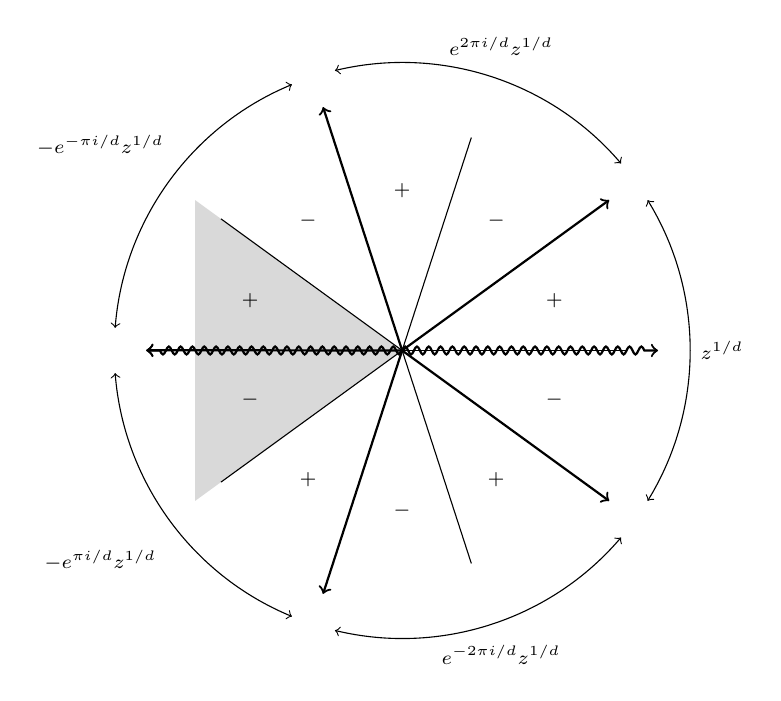
\begin{tikzpicture}[scale=3.25]
\fill[color=black!15](0.0,0.0)--(-0.809017,0.587785)--(-0.809017,-0.587785)--cycle;
\draw[->,black,thick](0.0,0.0)--(0.809017,0.587785);
\draw[-,black,thin](0.0,0.0)--(0.875,0.0);
\draw[->,black,thick](0.0,0.0)--(-0.309017,0.951057);
\draw[-,black,thin](0.0,0.0)--(0.27039,0.832174);
\draw[->,black,thick](0.0,0.0)--(-1.0,0.001);
\draw[-,black,thin](0.0,0.0)--(-0.70789,0.514312);
\draw[->,black,thick](0.0,0.0)--(-0.309017, -0.951057);
\draw[-,black,thin](0.0,0.0)--(0.27039, -0.832174);
\draw[->,black,thick](0.0,0.0)--(0.809017,-0.587785);
\draw[-,black,thin](0.0,0.0)--(-0.70789,-0.514312);
\draw[->,black,thick,decorate,decoration={coil,aspect=0.01,amplitude=.5mm, segment
length=1.5mm,post length=0.5mm}](0.0,0.0)--(1.0,0.0);
\draw[->,black,thick,decorate,decoration={coil,aspect=0.01,amplitude=.5mm, segment
length=1.5mm,post length=0.5mm}](0.0,0.0)--(-1.0,0.0);
\draw[] (1.25,0.0) node[black] {\scriptsize $z^{1/d}$};
\draw[] (0.386271, 1.18882) node[black] {\scriptsize $\ee^{2\pi i/d} z^{1/d}$};
\draw[] (-1.18, 0.8) node[black] {\scriptsize $-\ee^{-\pi i/d} z^{1/d}$};
\draw[] (-1.18, -0.82) node[black] {\scriptsize $-\ee^{\pi i/d} z^{1/d}$};
\draw[] (0.386271, -1.18882) node[black] {\scriptsize $\ee^{-2\pi i/d} z^{1/d}$};
\draw[] (0.59441, 0.193136) node[black] {\scriptsize $+$};
\draw[] (0.00000, 0.625000) node[black] {\scriptsize $+$};
\draw[] (-0.59441, 0.193136) node[black] {\scriptsize $+$};
\draw[] (-0.367366, -0.505636) node[black] {\scriptsize $+$};
\draw[] (0.367366, -0.505636) node[black] {\scriptsize $+$};
\draw[] (0.59441, -0.193136) node[black] {\scriptsize $-$};
\draw[] (0.00000, -0.625000) node[black] {\scriptsize $-$};
\draw[] (-0.59441, -0.193136) node[black] {\scriptsize $-$};
\draw[] (-0.367366, +0.505636) node[black] {\scriptsize $-$};
\draw[] (0.367366, +0.505636) node[black] {\scriptsize $-$};
\draw[<->](0.95922, -0.587811)arc(-31.5:31.5:1.125);
\draw[<->](0.855457, 0.730629)arc(40.5:103.5:1.125);
\draw[<->](-0.430519, 1.03936)arc(112.5:175.5:1.125);
\draw[<->](-1.12153, -0.0882665)arc(184.5:247.5:1.125);
\draw[<->](-0.262626, -1.09392)arc(256.5:319.5:1.125);
\end{tikzpicture}
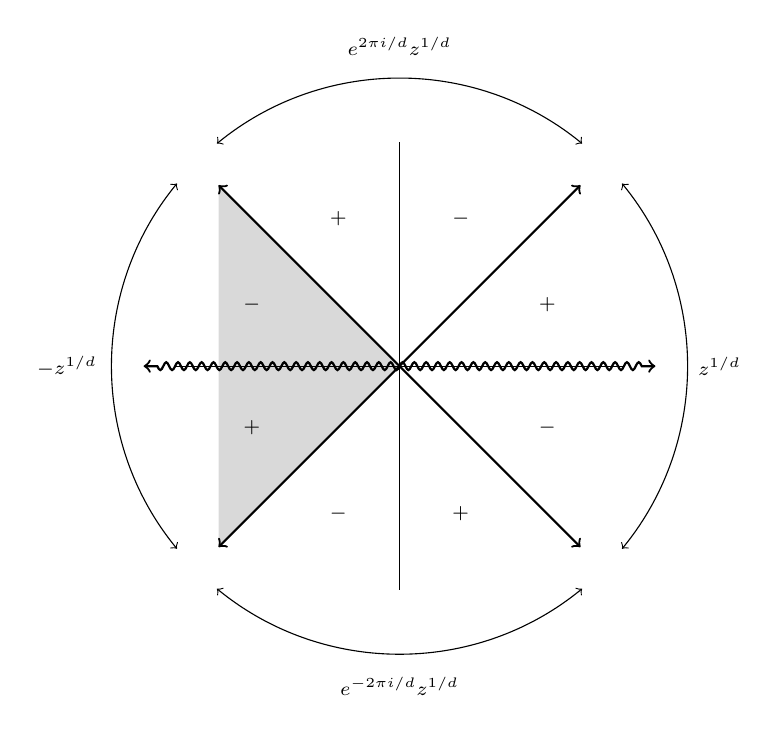
\begin{tikzpicture}[scale=3.25]
\fill[color=black!15](0.0,0.0)--(-0.707107,0.707107)--(-0.707107,-0.707107)--cycle;
\draw[->,black,thick](0.0,0.0)--(0.707107,0.707107);
\draw[-,black,thin](0.0,0.0)--(0.875,0.0);
\draw[->,black,thick](0.0,0.0)--(-0.707107,0.707107);
\draw[-,black,thin](0.0,0.0)--(0.0,0.875);
\draw[->,black,thick](0.0,0.0)--(-0.707107,-0.707107);
\draw[-,black,thin](0.0,0.0)--(-0.875,0.0);
\draw[->,black,thick](0.0,0.0)--(0.707107,-0.707107);
\draw[-,black,thin](0.0,0.0)--(0.0, -0.875);
\draw[->,black,thick,decorate,decoration={coil,aspect=0.01,amplitude=.5mm, segment
length=1.5mm,post length=0.5mm}](0.0,0.0)--(1.0,0.0);
\draw[->,black,thick,decorate,decoration={coil,aspect=0.01,amplitude=.5mm, segment
length=1.5mm,post length=0.5mm}](0.0,0.0)--(-1.0,0.0);
\draw[] (1.25,0.0) node[black] {\scriptsize $z^{1/d}$};
\draw[] (0.0, 1.25) node[black] {\scriptsize $\ee^{2\pi i/d} z^{1/d}$};
\draw[] (-1.3, 0.0) node[black] {\scriptsize $-z^{1/d}$};
\draw[] (0.0, -1.25) node[black] {\scriptsize $\ee^{-2\pi i/d} z^{1/d}$};
\draw[] (0.577425, 0.239177) node[black] {\scriptsize $+$};
\draw[] (-0.239177, 0.577425) node[black] {\scriptsize $+$};
\draw[] (-0.577425, -0.239177) node[black] {\scriptsize $+$};
\draw[] (0.239177, -0.577425) node[black] {\scriptsize $+$};
\draw[] (0.577425, -0.239177) node[black] {\scriptsize $-$};
\draw[] (-0.239177, -0.577425) node[black] {\scriptsize $-$};
\draw[] (-0.577425, +0.239177) node[black] {\scriptsize $-$};
\draw[] (0.239177, +0.577425) node[black] {\scriptsize $-$};
\draw[<->](0.869637, -0.713692)arc(-39.375:39.375:1.125);
\draw[<->](0.713692, 0.869637)arc(50.625:129.375:1.125);
\draw[<->](-0.869637, 0.713692)arc(140.625:219.375:1.125);
\draw[<->](-0.713692, -0.869637)arc(230.625:309.375:1.125);
\end{tikzpicture}
\end{center}
\caption{$f_{\zeta}$ glue and cuts for $d$ odd (Left) and $d$ even (Right)}
\label{stars}
\end{figure}

Therefore, we will continue determining the connection coefficients on each of the two half planes $\mathbb{C}_{-} = \{z |\Im z < 0\}$, where $\pm=-1$, and $\mathbb{C}_{+} = \{z |\Im z > 0\}$, where $\pm=+1$,
and leave the determination of the connection coefficients on $\mathbb{R}$, which is largely a matter of convention, to the next section. For a given $d^{\text{th}}$ root of unity $\zeta$ (and $z \in \mathbb{C} \setminus \mathbb{R}$), determine the even integer $\ell$ from $\pi \ell =\mp d \arg(\zeta^{\mp1})$ and the integer $k$ from $\pi k =\mp d \arg(-\zeta^{\mp1})$. The $f_{\zeta}$ in the $F_{\beta}$ basis are given by
\begin{equation}
\label{fzeta}
f_{\zeta}(z) = \frac{\ee^{\pi \ii \operatorname{sgn}(\ell \pm 1) (\frac{d-1}{2}-\sigma)}}{d^{-\frac{1}{2}}(2\pi)^{\frac{d-1}{2}}} \left(\frac{\Gamma(1-\bfb)}{\Gamma(1-\bfa)} F_1(z) + \sum_{j=1}^{q} \ee^{k \pi i (1-b_j)}\frac{\Gamma(b_j - (1,\hat{\bfb}_j))}{\Gamma(b_j-\bfa)} F_{b_j}(z) \right) \text{.}
\end{equation}
We will prove this first for the asymptotically smallest solution on each half plane, which corresponds to the shaded region in Figure \ref{stars}. Note that since these regions straddle $\mathbb{R}_{-}$, they correspond to two different values of $\zeta$ when $d$ is odd. We would like to show these solutions in the $F_{\beta}(z)$ basis are
\begin{align*}
f_{-1}(z) &= \eqref{fzeta} \text{ with } \operatorname{sgn}(\ell \pm 1) = \mp\text{, and } k = 0\text{,} \quad & d \text{ even}\text{,}\\
f_{-\ee^{\mp\pi i/d}}(z) &= \eqref{fzeta} \text{ with } \operatorname{sgn}(\ell \pm 1) = \pm\text{, and } k = \mp \text{,} \quad & d \text{ odd}\text{.}
\end{align*}
These identities follow by observing that the parenthesized sum in \eqref{fzeta} is the sum of all $s$-residues of
\begin{equation*}
-\frac{\Gamma(1-s-(1,\bfb))}{\Gamma(1-s-\bfa)} z^s \times \begin{cases}
1\text{,} & d \text{ even}\\
\ee^{\mp \pi i s}\text{,} & d \text{ odd}
\end{cases}\text{.}
\end{equation*}
The asymptotic value of the integral around all poles can be deduced by deforming the contour to an essentially vertical one passing through the saddle point near $s=-z^{1/d}$ and tending to $\pm \ii \infty$ along a path of steep descent (Lemma \ref{lamma_minimal_asmp}). The equality holds due to the uniqueness of the minimal solution.

\begin{lemma}
\label{lamma_minimal_asmp}
As $x \to \infty$ (from $\mathbb{R}$),
\begin{equation*}
\int_{-\ii \infty}^{+\ii \infty} \frac{\Gamma(1-\bfb + s) \Gamma(s)}{\Gamma(1-\bfa+s)} x^{-d s} \frac{\dd s}{2\pi \ii} \sim d^{-\frac{1}{2}}(2\pi)^{\frac{d-1}{2}} \ee^{-d x} x^{\frac{d-1}{2} - \sigma}\text{.}
\end{equation*}
\end{lemma}
\begin{proof}
Using $\logG (1-a+s) = s \log s - s + (\tfrac{1}{2}-a) \log s + \frac{1}{2} \log(2\pi) + O(s^{-1})$, the integrand is
\begin{equation*}
\frac{\Gamma(1-\bfb + s) \Gamma(s)}{\Gamma(1-\bfa+s)} x^{-d s} = \ee^{d s (\log s - \log x-1) + (\frac{d-2}{2}-\sigma) \log s} \left( (2\pi)^{\frac{d}{2}} + O(s^{-1}) \right)
\end{equation*}
With $s = x \ee^{\ii \theta}$ in the middle integral, the path between $\pm \ii \infty$ can be decomposed as
\begin{equation*}
\int_{-\ii \infty}^{+\ii \infty} \dots \frac{\dd s}{2\pi \ii} = \int_{-\ii \infty}^{- \ii x} \dots \frac{\dd s}{2\pi \ii} + \int_{-\frac{\pi}{2}}^{+\frac{\pi}{2}} \dots \frac{x \ee^{\ii \theta} \dd \theta}{2\pi} + \int_{+\ii x}^{+\ii \infty} \dots \frac{\dd s}{2\pi \ii}\text{.}
\end{equation*}
The outer two integrals are much smaller than the claimed main term, so it is enough to focus on the integral over the half-circle.
\begin{align*}
\int_{-\ii \infty}^{+\ii \infty} \frac{\Gamma(1-\bfb + s) \Gamma(s)}{\Gamma(1-\bfa)} x^{-d s} \frac{\dd s}{2\pi \ii} & \sim (2\pi)^{\frac{d}{2}} \int_{-\frac{\pi}{2}}^{+\frac{\pi}{2}} \ee^{d x e^{\ii \theta} (\ii \theta-1) + (\frac{d-2}{2}-\sigma)(\log x + \ii \theta)} \frac{x \ee^{\ii \theta} \dd \theta}{2\pi}\\
& = (2\pi)^{\frac{d-2}{2}} \ee^{-d x} x^{\frac{d}{2} -\sigma} \int_{-\frac{\pi}{2}}^{+\frac{\pi}{2}} \ee^{d x (e^{\ii \theta} \ii \theta + 1-\ee^{\ii \theta}) + (\frac{d-2}{2}-\sigma) \ii \theta} \dd \theta\\
(\text{set } t = \theta \sqrt{dx} ) \quad \quad & \sim d^{-\frac{1}{2}} (2\pi)^{\frac{d-1}{2}} \ee^{-d x} x^{\frac{d-1}{2} -\sigma} \int_{-\frac{\pi}{2}\sqrt{dx}}^{+\frac{\pi}{2}\sqrt{dx}} \frac{\ee^{-\frac12 t^2}}{\sqrt{2\pi}} \dd t\text{.}
\end{align*}
\end{proof}

Now, since the $F_{\beta}(z)$ are either entire or have simple prefactors as $z$ makes one trip around the origin, it is a simple matter to transform these minimal solutions back to an arbitrary $f_{\zeta}(z)$ by moving $z$ around the origin a few times in either direction and using the $\mathbb{C}_{+}$ and $\mathbb{C}_{-}$ gluings in point 5. This gives \eqref{fzeta} and these $d$ expansions along with the $p$ expansions in \eqref{algasymp} give a $(d+p)\times(d+p)$ matrix whose inverse has first row
\begin{equation}
\label{entirerecp2}
\begin{alignedat}{1}
\FF{p}{F}{q}{\mathbf{a}}{\mathbf{b}}{z}&=\sum_{i=1}^{p} \frac{\Gamma(\mathbf{b}) \Gamma(\hat{\mathbf{a}}_i-a_i)}{\Gamma(\hat{\mathbf{a}}_i)\Gamma(\mathbf{b}-a_i)} (-z)^{-a_i} \FFe{q+1}{F}{p-1}{-}{a_i,1+a_i-\mathbf{b}}{1+a_i-\hat{\mathbf{a}}_i}{\frac{(-1)^d}{z}}\\
&+\sum_{\zeta^d=1} c^{(\pm)} (\zeta |\bfa; \bfb) \frac{\Gamma(\mathbf{b})}{d^{\frac{1}{2}} (2 \pi )^{\frac{d-1}{2}} \Gamma(\mathbf{a})} \ee^{d \zeta z^{1/d}}(\zeta z^{1/d})^{\frac{d-1}{2}-\sigma} \FFe{p}{U}{q}{-}{\bfa}{\bfb}{\frac{1}{\zeta z^{1/d}}}\text{,}
\end{alignedat}
\end{equation}
and this is the correct form of \eqref{entirerecp}. The $c^{(\pm)}(\zeta)$ here are interesting combinatorial exponential sums: with the even integer $\ell$ determined uniquely as before from $\pi \ell = \mp d \arg(\zeta^{\mp1})$, they are
\begin{equation}
\label{equ_czeta}
c^{(\pm)} (\zeta |\bfa; \bfb) =\sum_{\substack{0 \le n_1, \dots, n_p \\ 0 \le m_1, \dots, m_q \le 1 \\ \Sigma \bfn + \Sigma \bfm = (|\ell \pm 1|-1)/2}}{ \ee^{2\pi \ii \operatorname{sgn}\left(\ell\pm 1\right) (\bfn \cdot \bfa + \mathbf{m} \cdot (\bfb + \frac{1}{2}))}}\text{.}
\end{equation}
The form of these exponential sums follows from, for any $p \ge 1$, $\bfx \in \mathbb{C}^p$, $\bfy \in \mathbb{C}^q$ and $0 \le w \le q$,
\begin{align*}
\sum_{\substack{0 \le n_1, \dots, n_p \\ 0 \le m_1, \dots, m_q \le 1 \\ \Sigma \bfn + \Sigma \bfm = w}}{ \bfx^\bfn (-\bfy)^\bfm} &= \sum_{j=1}^{p}\sum_{i=0}^{w} \frac{x_j^{i+p-1} \Pi_{w-i}(-\bfy)}{\Pi (x_j-\hat{\bfx}_j)}\\
&=\sum_{j=1}^{p} \sum_{i=1}^{q} \frac{x_j^{p-1} \Pi_w(-\hat{\bfy}_i) \Pi(x_j-\hat{\bfy}_i)}{\Pi(x_j - \hat{\bfx}_j) \Pi (y_i-\hat{\bfy}_i)}\text{, for } w < q\text{,}
\end{align*}
which arise when inverting the matrix. Here, $\bfx^{\bfn} = \prod_i x_i^{n_i}$, $\Pi(\bfx)$ gives the product of the $x_i$, and $\Pi_w(\bfx)$ is the $w^{\text{th}}$ symmetric polynomial in the $x_i$. See, for example, Lemma \ref{lemmatrig} below.

\subsubsection{partial fraction derivation}
Lemma \ref{lamma_minimal_asmp} gives integral representations of the the $d$ asymptotic solutions. For each $j$ ranging from $1-d$ to $d-1$ in steps of $2$, set the corresponding $\zeta = -\ee^{\pm \pi \ii \frac{j-1}{d}}$. Then, these $d$ solutions are given by
\begin{gather*}
\int_{-\ii \infty}^{+\ii \infty} \frac{\Gamma(1-(1,\bfb)-s)}{\Gamma(1-\bfa-s)} \ee^{\pm j \pi s} (-z)^s \frac{\dd s}{2\pi \ii} = 
\ee^{\pm \pi \ii \operatorname{sgn}(j-\frac{1}{2}) (\frac{d-1}{2}-\sigma)} d^{-\frac{1}{2}} (2\pi)^{\frac{d-1}{2}} \times \\
\ee^{d \zeta z^{1/d}}(\zeta z^{1/d})^{\frac{d-1}{2}-\sigma} \FFe{p}{U}{q}{-}{\bfa}{\bfb}{\frac{1}{\zeta z^{1/d}}}\text{,}
\end{gather*}
and the $p$ algebraic asymptotic solutions are given by
\begin{gather*}
\int_{-\ii \infty}^{+\ii \infty} \frac{\Gamma(1-(1,\bfb)-s)\Gamma(a_i+s)}{\Gamma(1-\hat{\bfa}_i-s)} ((-1)^d)^{\pm (a_i+s)} (-z)^s \frac{ds}{2\pi \ii} =
\frac{\Gamma(1+a_i-(1,\bfb))}{\Gamma(1+a_i-\hat{\bfa}_i)} \times \\
(-z)^{-a_i} \FFe{q+1}{F}{p-1}{-}{a_i,1+a_i-\mathbf{b}}{1+a_i-\hat{\mathbf{a}}_i}{\frac{(-1)^d}{z}}\text{.}
\end{gather*}
We would like to express
\begin{equation*}
\frac{\Gamma(\mathbf{a})}{\Gamma(\mathbf{b})}\FF{p}{F}{q}{\mathbf{a}}{\mathbf{b}}{z} = \int_{-\ii \infty}^{+\ii \infty} \frac{\Gamma(\mathbf{a}+s) \Gamma(-s)}{\Gamma(\mathbf{b}+s)} (-z)^s \frac{\dd s}{2\pi \ii}
\end{equation*}
as a linear combination of the above. This is implied by
\begin{equation*}
\frac{\Gamma(\mathbf{a}+s)}{\Gamma(\mathbf{b}+s)} = \sum_{i=1}^{p} h_i \frac{\Gamma(1-\bfb-s)\Gamma(a_i+s)}{\Gamma(1-\hat{\bfa}_i-s)} ((-1)^d)^{\pm (a_i+s)} + \sum_{\zeta^d = 1} g_{\zeta} \frac{\Gamma(1-\bfb-s)}{\Gamma(1-\bfa-s)} \ee^{\pm j \pi s}\text{,}
\end{equation*}
or
\begin{equation*}
\pi^{p-q} \frac{\sin \pi(\bfb + s) } {\sin \pi(\bfa + s)}
 = \sum_{i=1}^{p} h_i \frac{((-1)^d)^{\pm (a_i+s)} \pi}{\sin \pi(a_i+s)} + \sum_{\zeta^d = 1} g_{\zeta} \ee^{\pm j \pi s}\text{.}
\end{equation*}
Both sides are multiplied by $(-1)^{d+1}$ as $s \to s+1$. The residue at $s=-a_i$ gives
\begin{equation*}
h_i = \pi^{p-q-1} \frac{\sin \pi(\bfb + s) }{\sin \pi(\hat{\bfa}_i - a_i) } = \frac{\Gamma(\hat{\bfa}_i- a_i)\Gamma(1+ a_i-\hat{\bfa}_i)}{\Gamma(\hat{\bfb}_i- a_i)\Gamma(1+ a_i-\hat{\bfb}_i)}\text{.}
\end{equation*}
The coefficients of the remaining trigonometric polynomial can be found via power series, leading to
\begin{align*}
[x^k] \frac{\prod_{j=1}^{q} {1- \ee^{+2\pi \ii b_j}x}}{\prod_{i=1}^{p} {1- \ee^{+2\pi \ii a_i} x}} &= \begin{cases} c^{(+)}(\ee^{+\frac{2\pi \ii (k+0)}{d}} | \bfa, \bfb)\text{, for } k \le \frac{d-1}{2} \\
c^{(-)}(\ee^{+\frac{2\pi \ii (k+1)}{d}} | \bfa, \bfb)\text{, for } k \le \frac{d-2}{2}
\end{cases}\text{,}\\
[x^k] \frac{\prod_{j=1}^{q} {1- \ee^{-2\pi \ii b_j}x}}{\prod_{i=1}^{p} {1- \ee^{-2\pi \ii a_i} x}} &= \begin{cases} c^{(-)}(\ee^{-\frac{2\pi \ii (k+0)}{d}} | \bfa, \bfb)\text{, for } k \le \frac{d-1}{2} \\
c^{(+)}(\ee^{-\frac{2\pi \ii (k+1)}{d}} | \bfa, \bfb)\text{, for } k \le \frac{d-2}{2}
\end{cases}\text{,}
\end{align*}
which agrees with the previous formula \eqref{equ_czeta}.


\subsection{real problems}
Being the sum of $q+1$ discontinuous functions, the right hand side of \eqref{entirerecp2} miraculously represents a continuous function. Here we simply make the observation that \eqref{entirerecp2} remains valid if $\pm = \tfrac{1}{\pi i}(\log(z)-\log(-z))$ (and the $F_{b_j}(z)$) retain the standard counterclockwise continuity on $\mathbb{R}$ and the functions ${}_{q+1}F_{p-1}$ and ${}_p U_{q}$ are evaluated with the nonstandard clockwise continuity. This is already present in $\eqref{algasymp}$ for ${}_{q+1}F_{p-1}^{-}$, and \eqref{fzeta} gives $f_{\zeta}(z)$ the counterclockwise continuity, which gives ${}_p U_q$ the clockwise continuity: ${}_{q+1}F_{p-1}$ and ${}_p U_{q}$ need the clockwise continuity simply because $1/z$ flips the orientation.

There are many problems with the asymptotic formula for ${}_p F_{q}(z)$ on $\mathbb{R}$. First, on $z>0$ the asymptotically largest exponential term has a discontinuity due to that of ${}_p U_{q}(z)$. Then, on $z<0$ the smallest exponential term has a discontinuity arising from the algebraic prefactor. The non-exponential algebraic terms also have discontinuities on either side of $\mathbb{R}$ depending on the parity of $d$. Finally, the most serious problem is that \eqref{entirerecp2} implies that ${}_p F_{q}(z)$ has infinitely many zeros in any sector $|\arg(-z)| < \epsilon$ for $d>2$, and thus near $z<0$ massive cancellation among the components of the asymptotic formula is possible when $d>2$.

The bad situation near $z<0$ can be illustrated explicitly by continuing with the example of $\FFf{0}{F}{2}{\tfrac{1}{3},\tfrac{1}{2}}{z}$. For $x>0$ a rearrangement of the three terms of \eqref{entirerecp2} gives
\begin{equation}
\label{optimized}
\begin{aligned}
\FFf{0}{F}{2}{\tfrac{1}{3},\tfrac{1}{2}}{-x^3} &= \frac{\Gamma\left(\frac{1}{3}\right)}{\sqrt{3 \pi }} \ee^{3 x/2} x^{1/6} \cos \left(\frac{\pi}{18} + \frac{3 \sqrt{3}
   x}{2}\right)\frac{U(-\ee^{-2 \pi \ii/3}/x)+U(-\ee^{2 \pi \ii/3}/x)}{2}\\
&+\frac{\Gamma\left(\frac{1}{3}\right)}{\sqrt{3 \pi }} \ee^{3 x/2} x^{1/6} \sin \left(\frac{\pi }{18} + \frac{3 \sqrt{3}
   x}{2}\right)
   \frac{U(-\ee^{-2\pi \ii/3}/x)-U(-\ee^{2\pi \ii/3}/x)}{2\ii}\\
 &+\frac{\sqrt{3}}{2} \frac{\Gamma\left(\frac{1}{3}\right)}{\sqrt{3 \pi }} \ee^{-3x} x^{1/6} U(-1/x)
\text{.}
\end{aligned}
\end{equation}
What is to be gained from rewritting the formula this way? First, since the two fractions involving $U$ are just the real and imaginary parts of $U$, each of the three terms on the right hand side is a real number. Second, since $U(z) \sim 1-\frac{1}{108}z + \cdots$, it is clear that, as long as the value of the cosine is not too small, a good relative approximation for $x$ large is given by
\begin{equation*}
\FFf{0}{F}{2}{\tfrac{1}{3},\tfrac{1}{2}}{-x^3} \approx \frac{\Gamma\left(\frac{1}{3}\right)}{\sqrt{3 \pi }} e^{3 x/2} x^{1/6}
   \cos \left(\frac{\pi }{18} + \frac{3 \sqrt{3}
   x}{2}\right)
\end{equation*}
and that the zeros of $F(z)$ on $z<0$ occur approximately where the value of the cosine is zero. Finally, however, this formula does not help much in evaluating $F(z)$ near such a zero: the cosine term and sine term cannot be simultaneously small and hence must cancel each other out at a zero of $F(z)$. This is detailed in the following table, which shows how close the zeros of $F(-x^3)$ are to the zeros of the cosine, the magnitude of the first term in the ``optimized" formula \eqref{optimized} at the roots, and the magnitude of the first term in the plain formula \eqref{entirerecp2} also at the roots. With $x_n \approx 2\pi(9n+4)/(27 \sqrt{3})$ denoting the $n^{\text{th}}$ root of $F(-x^3)$ on $x>0$, we have

\begin{center}
\begin{tabular}{c|ccc}
$n$ & $\frac{\frac{2\pi(9n+4)}{27 \sqrt{3}} - x_n}{\frac{1}{324 x_n}}$ & $|$First term of \eqref{optimized}$|$ & $|$First term of \eqref{entirerecp2}$|$ \\[-2.0ex] \\ \hline \\ [-2ex]
 $20$ & $0.9805$ & $6.024\cdot10^{12}$ & $9.472\cdot10^{15}$ \\
 $25$ & $0.9843$ & $4.375\cdot10^{16}$ & $8.529\cdot10^{19}$ \\
 $30$ & $0.9869$ & $3.280\cdot10^{20}$ & $7.630\cdot10^{23}$ \\
 $35$ & $0.9887$ & $2.513\cdot10^{24}$ & $6.794\cdot10^{27}$ \\
 $40$ & $0.9901$ & $1.957\cdot10^{28}$ & $6.030\cdot10^{31}$ \\
 $45$ & $0.9912$ & $1.544\cdot10^{32}$ & $5.338\cdot10^{35}$ \\
 $50$ & $0.9921$ & $1.230\cdot10^{36}$ & $4.715\cdot10^{39}$
\end{tabular}
\end{center}
In conclusion, the real roots of $\FFf{0}{F}{2}{\tfrac{1}{3},\tfrac{1}{2}}{-x^3}$ are a distance of approximately $\tfrac{1}{324} x^{-1}$ away from the roots of the cosine and the optimized formula only reduces the size of the first term by a miniscule amount. Suppose we are at a root $z=-x^3$ of $\FFf{0}{F}{2}{\tfrac{1}{3},\tfrac{1}{2}}{z}$ and would like to prove numerically that $|\FFf{0}{F}{2}{\tfrac{1}{3},\tfrac{1}{2}}{-x^3}|<2^{-m}$. Since
\begin{align*}
|\text{first term of \eqref{entirerecp2}}| &\approx \frac{\Gamma(\tfrac13)}{2 \sqrt{3 \pi}} \ee^{3x/2} x^{1/6}\text{,}\\
|\text{first term of \eqref{optimized}}| &\approx \frac{\Gamma(\tfrac13)}{216 \sqrt{\pi}} \ee^{3x/2} x^{-5/6}\text{,}
\end{align*}
the formulas \eqref{entirerecp2} and \eqref{optimized} require $O(x+m)$ bits of the $U$-factors, and thus are no better than \eqref{Fdef}, which requires at least $O(x)$ terms.

\section{The $G$ function}

\newcommand{\bfalpha}[0] {\pmb{\alpha}}
\newcommand{\bfgamma}[0] {\pmb{\gamma}}
\newcommand{\bfbeta}[0]  {\pmb{\beta}}
\newcommand{\bfdelta}[0] {\pmb{\delta}}

The parameters are
\begin{itemize}
\item{$0 \le n \le p$ and $0 \le m \le q$}
\item{$\bfa = (\bfalpha, \bfgamma) \in \mathbb{C}^{p}$, $\bfalpha = a_1, \dots, a_n$, $\bfgamma = a_{n+1}, \dots, a_p$}
\item{$\bfb = (\bfbeta, \bfdelta) \in \mathbb{C}^{q}$, $\bfbeta = b_1, \dots, b_m$, $\bfdelta = b_{m+1}, \dots, b_q$}
\item{$a_i-b_j \neq 1, 2, \dots$ for any $i \le n$ and $j \le m$, that is, $\Gamma(1-\bfalpha+s)$ and $\Gamma(\bfbeta-s)$ share no poles.}
\item{$z \in \mathbb{C}$ with $z \neq 0$}
\end{itemize}
The possible paths in the definition $ G_{p,q}^{m,n} (z |\bfalpha, \bfgamma; \bfbeta, \bfdelta) = \int \frac{\Gamma(\bfbeta-s)\Gamma(1-\bfalpha+s)}{\Gamma(1-\bfdelta+s)\Gamma(\bfgamma-s)}z^s\frac{ds}{2 \pi \ii}$ are
\begin{enumerate}
\item{from $-\ii \infty$ to $+ \ii \infty$, separating the poles of $\Gamma(1-\bfalpha+s)$ from those of $\Gamma(\bfbeta-s)$, converges for $|\arg(z)| < (m+n-\tfrac{1}{2}(p+q)) \pi$}
\item{encircle the poles of $\Gamma(\bfbeta-s)$ clockwise}
\item{encircle the poles of $\Gamma(1-\bfalpha+s)$ counterclockwise}
\end{enumerate}
By the shift $s \to s+1$, the function $G((-1)^{p-m-n}z)$ is a solution to a hypergeometric differential equation:
\begin{equation*}
(z \partial_z - b_1)\cdots (z \partial_z - b_q)-(z \partial_z - a_1) \cdots (z \partial_z - a_p) z = 0\text{.}
\end{equation*}
Thus it suffices to connect it to some ${}_p F_q$ \footnote{or limiting cases thereof}.

\subsection{The case $q>p$}
Set $d = q-p$. Path 2 gives
\begin{equation}
\label{eq_Gpath2}
G(z) = \sum_{j=1}^{m} \frac{\Gamma(\hat{\bfbeta}_j - b_j)\Gamma(1+b_j-\bfalpha)}{\Gamma(\bfgamma-b_j)\Gamma(1+b_j-\bfdelta)} z^{b_j}\FF{p}{F}{q-1}{1+b_j-\bfa}{1+b_j-\hat{\bfb}_j}{(-1)^{p-m-n}z}\text{,}
\end{equation}
and this is useful if $|z|$ is not too large. We need the asymptotic expansion of $G(z)$ for large $z$. What is interesting here is that the poles of $\Gamma(1-\bfalpha+s)$ do not even give a hint of the correct algebraic portion; we have from \eqref{entirerecp2},
\begin{align*}
G((-1)^{p-m-n}z) &= \sum_{i=1}^{n} \frac{h_{i}^{(\pm)}(\bfalpha, \bfgamma; \bfbeta, \bfdelta)}{(2\pi \ii)^{p-n} } \frac{\Gamma(a_i-\hat{\bfa}_i)\Gamma(1-a_i+\bfbeta)}{\Gamma(a_i-\bfdelta)} (-z)^{a_i-1}\FF{q}{F}{p-1}{1-a_i+\bfb}{1-a_i+\hat{\bfa}_i}{\frac{(-1)^{d}}{z}}\\
&+\sum_{\zeta^d=1} \frac{g_{\zeta}^{(\pm)}(\bfalpha, \bfgamma; \bfbeta, \bfdelta)}{d^{\frac{1}{2}} (2\pi)^{\frac{d-1}{2}} (2\pi \ii)^{1+p-m-n}} \ee^{d \zeta z^{1/d}}(\zeta z^{1/d})^{\Sigma \bfb - \Sigma \bfa - \frac{d-1}{2}} \FF{p}{U}{q-1}{1+b_j-\bfa}{1+b_j-\hat{\bfb}_j}{\frac{1}{\zeta z^{1/d}}}\text{,}
\end{align*}
where the ${}_p U_{q-1}$s on the right hand side are independent of the choice of $j$ (Lemma \ref{lemma_pUq_inv}), and the $h_i$ and $g_{\zeta}$ are entire functions of the parameters.
\begin{align*}
h_{i}^{(\pm)}\left(\begin{array}{c} \bfalpha, \bfgamma \\ \bfbeta, \bfdelta \end{array}\right) &= \sum_{j=1}^{m} \frac{\sin \pi (b_j-\bfgamma) \sin \pi (a_i-\hat{\bfbeta}_j)}{\sin \pi (b_j-\hat{\bfbeta}_j)} (2 \ii)^{p-n} \times \begin{cases} 1\text{,}& p-m-n \text{ odd}\\
-\ee^{\pm \pi \ii b_j}\text{,}& p-m-n \text{ even}\end{cases}\\
&= \ee^{-\pi \ii (\Sigma \bfgamma + (m-1) a_i)} \times \text{some Laurent polynomial in } \ee^{2\pi \ii (\bfa, \bfb)}
\end{align*}
\begin{align*}
g_{\zeta}^{(\pm)}\left(\begin{array}{c} \bfalpha, \bfgamma \\ \bfbeta, \bfdelta \end{array}\right) &= \sum_{j=1}^{m} \frac{\sin \pi (\bfgamma - b_j) \, c_{\zeta}^{(\pm)}(-\bfa; -\hat{\bfb}_j)}{\sin \pi (\hat{\bfbeta}_j-b_j)} (2 \ii)^{1+p-m-n} \times \begin{cases} \ee^{-\operatorname{pm}(\mp \zeta^{\mp})\pi \ii b_j}\text{,}& p-m-n \text{ odd}\\
\ee^{(\operatorname{pm}(\pm \zeta^{\mp}) \pm 1) \pi \ii b_j}\text{,}& p-m-n \text{ even}\end{cases}\\
&= \ee^{-\pi \ii (\Sigma \bfgamma + \Sigma \bfbeta)} \times \text{some Laurent polynomial in } \ee^{2\pi \ii (\bfa, \bfb)}
\end{align*}
where $\operatorname{pm}(w) := \frac{1}{\pi \ii}(\log(w)-\log(-w))$ so that $\pm = \operatorname{pm}(z)$. The general form of these polynomials is too complicated to be of use: they should be generated once the parameters counts $m,n,p,q$ are fixed. The following lemma is useful to see that the above trigonometric sums with denominator are in fact entire exponential sums.
\begin{lemma}
\label{lemmatrig}
Set $\bfx = x_1, ..., x_m$ with $m \ge 1$. For any integer $k$,
\begin{equation*}
\sum_{i=1}^{m} \frac{x_i^k}{\Pi(x_i-\hat{\bfx}_i)} = \begin{cases} \sum\limits_{\substack{n_1, \dots, n_m \ge 0 \\ \Sigma \bfn = k+1-m}} \bfx^\bfn \text{,} & k \ge 0\\
\sum\limits_{\substack{n_1, \dots, n_m < 0 \\ \Sigma \bfn = k+1-m}} \bfx^{\bfn} (-1)^{m-1} \text{,} & k < 0
\end{cases}
\end{equation*}
\end{lemma}
\begin{proof}
Multiplying both sides by $y^k$ and summing over all $k \ge 0$ turns the right hand side into $y^{m-1} / \Pi(1-y\bfx)$ and the left and side into its partial fraction decomposition. The case $k < 0$ follows similarly.
\end{proof}

\subsection{The case $q<p$}
Path 3 gives
\begin{equation}
\label{eq_Gpath3}
G(z) = \sum_{i=1}^{n} \frac{\Gamma(a_i-\hat{\bfalpha}_i)\Gamma(1-a_i+\bfbeta)}{\Gamma(a_i-\bfdelta)\Gamma(1-a_i+\bfgamma)} z^{a_i-1}\FF{q}{F}{p-1}{1-a_i+\bfb}{1-a_i+\hat{\bfa}_i}{\frac{(-1)^{q-m-n}}{z}}\text{,}
\end{equation}
and this is useful if $|z|$ is not too small. However, since $G(z|\bfa; \bfb) = G(1/z|1-\bfb; 1-\bfa)$ modulo branch cut issues, there is no need whatsoever to consider this case.

\subsection{The case $q=p$}
The function is in general discontinuous on the unit circle. The expansion \eqref{eq_Gpath2} is valid for $|z| < 1$, and \eqref{eq_Gpath3} is valid for $|z| > 1$.



\section{Bilateral series}
The F series is a sum over Half of the integers. Accordingly, there is an H series which sums over the Full set of integers: we have ${}_p H_q(\bfa; \bfb|z)$ defined as the formal sum of $z^n (\bfa)_n/(\bfb)_n$ over \emph{all} $n$. Specifically,
\begin{equation*}
\FF{p}{H}{q}{\bfa}{\bfb}{z} := \FF{p+1}{F}{q}{\bfa,1}{\bfb}{z}-1 + \FFe{q+1}{F}{p}{-}{1-\bfb,1}{1-\bfa}{\frac{(-1)^{p-q}}{z}} \text{,}
\end{equation*}
with a similar definition of $H^{-}$. This gives ${}_p H_q(z)$ a branch cut along $[0,\infty]$ for $p\ge q$ and along $[0,(-1)^{p-q} \infty]$ for $p < q$, and we immedately have ${}_p H_q (\bfa; \bfb | z) = {}_q H_p^{-} (1-\bfb; 1-\bfa | (-1)^{p-q}/z)$. In terms of convergent series, \eqref{balanced_outside} gives
\begin{align*}
\FF{p}{H}{q}{\bfa}{\bfb}{z} &= \sum_{i=1}^p \frac{\Gamma(\bfb)\Gamma(1-a_i)}{\Gamma(\hat{\bfa}_i)}\frac{\Gamma(\hat{\bfa}_i-a_i)}{\Gamma(\bfb-a_i)} (-z)^{-a_i} \FFe{q}{F}{p-1}{-}{1+a_i-\bfb}{1+a_i-\hat{\bfa}_i}{\frac{(-1)^{p-q}}{z}}\text{,} \quad p \ge q \text{,}\\
\FF{p}{H}{q}{\bfa}{\bfb}{(-1)^{p-q}z} &= \sum_{i=1}^q \frac{\Gamma(1-\bfa)\Gamma(b_i)}{\Gamma(1-\hat{\bfb}_i)}\frac{\Gamma(b_i-\hat{\bfb}_i)}{\Gamma(b_i-\bfa)} (-z)^{1-b_i} \FF{p}{F}{q-1}{1+\bfa-b_i}{1+\hat{\bfb}_i-b_i}{(-1)^{p-q}z}\text{,} \quad p \le q \text{,}
\end{align*}
with the special cases ${}_0 H_1(b|z) = \Gamma(b) z^{1-b} \ee^{z}$,
 \begin{equation}
\label{equ_1H1}
\Head{1}{H}{1} \Arg{a}{b}{z} = \frac{\Gamma(1-a)\Gamma(b)}{\Gamma(b-a)} (-z)^{1-b}(1-z)^{b-a-1}\text{,}
\end{equation}
\begin{equation}
\label{equ_2H2}
\begin{aligned}
\FF{2}{H}{2}{a_1,a_2}{b_1,b_2}{z} &= \frac{\Gamma(1-a_1)\Gamma(1-a_2)\Gamma(b_1)\Gamma(b_1-b_2)}{\Gamma(1-b_2)\Gamma(b_1-a_1)\Gamma(b_1-a_2)} (-z)^{1-b_1} \FF{2}{F}{1}{1+a_1-b_1,1+a_2-b_1}{1+b_2-b_1}{z}\\
&+ \frac{\Gamma(1-a_1)\Gamma(1-a_2)\Gamma(b_2)\Gamma(b_2-b_1)}{\Gamma(1-b_1)\Gamma(b_2-a_1)\Gamma(b_2-a_2)} (-z)^{1-b_2} \FF{2}{F}{1}{1+a_1-b_2,1+a_2-b_2}{1+b_1-b_2}{z}\text{.}
\end{aligned}
\end{equation}
Assuming we are on the side of the branch cut where $\log(z-1) = \pm \pi i + \log(1-z)$, this, when combined with \eqref{nearone} gives (with $\sigma := b_1+b_2-a_1-a_2-1$)
\begin{align*}
\FF{2}{H}{2}{a_1,a_2}{b_1,b_2}{1-z} &= \frac{\Gamma(1-a_1)\Gamma(1-a_2)\Gamma(b_1)\Gamma(b_2)\Gamma(\sigma)}{\Gamma(b_1-a_1)\Gamma(b_1-a_2)\Gamma(b_2-a_1)\Gamma(b_2-a_2)}(1 + O(z))\\
&+ \Gamma(-\sigma) z^{\sigma} \left(\frac{\Gamma(b_1)\Gamma(b_2)}{\Gamma(a_1)\Gamma(a_2)} + \ee^{\mp \pi \ii \sigma} \frac{\Gamma(1-b_1)\Gamma(1-b_2)}{\Gamma(1-a_1)\Gamma(1-a_2)} + O(z)\right)\text{.}
\end{align*}


\section{The $\Gamma$ function}
For the definition of the $\Gamma$ function we will take
\begin{align*}
\Gamma(z+1) &:= \int_0^{\infty} t^z \ee^{-t} \dd t\text{,} \quad \Re z > -1\\
&= \lim_{r \to \infty} \int_0^{r} t^z (1-\tfrac{t}{r})^r \dd t \\
&= \lim_{r \to \infty} r^{z+1} \int_{0}^{1} t^z (1-t)^r \dd t \\
&= \lim_{r \to \infty} r^{z+1} \frac{r!}{(z+1) \cdots (z+r+1)} \\
&= \prod_{n=1} ^{\infty} \frac{(1+\frac{1}{n})^z}{1+\frac{z}{n}}\text{,}
\end{align*}
which gives a meromorphic continuation to $z \in \mathbb{C}$ and a clear definition of $\logG(z+1)$.

Substituting $u=t+s$ and $v=t/(t+s)$ into
\begin{equation*}
\Gamma(a) \Gamma(b) = \int_0^{\infty} \int_0^{\infty} t^{a-1} s^{b-1} \ee^{-t-s} \dd t \dd s
\end{equation*}
produces
\begin{equation}
\label{equ_beta_integral}
\frac{\Gamma(a) \Gamma(b)}{\Gamma(a+b)} = \int_0^1 v^{a-1}(1-v)^{b-1} \dd v\\
= \int_0^{\infty} \frac{w^a}{(1+w)^{a+b}} \frac{\dd w}{w}\text{.}
\end{equation}
Let $C$ be the contour that starts below the real axis at $+\infty -\epsilon \ii$, wraps clockwise around the origin, and returns above the real axis to $+\infty +\epsilon \ii$.
\begin{align*}
2\pi \ii (-1) &= \int_C \frac{(-t)^z \dd t}{(1+t)t} \quad \text{deform contour hitting residue at } t = -1  \\
&= \int_{\infty}^{0} \frac{e^{\pi \ii z} t^z \dd t}{(1+t)t} + \int_{0}^{\infty} \frac{e^{-\pi \ii z} t^z \dd t}{(1+t)t}\\
&= (-e^{\pi \ii z} + e^{-\pi \ii z}) \Gamma(z)\Gamma(1-z)\text{.}
\end{align*}
The resulting reflection formula $\Gamma(z)\Gamma(1-z) = \pi \csc \pi z$ holds for all $z$ by analytic continuation. This formula also gives a formula for the entire function
\begin{equation}
\label{equ_gamma_hankel}
\frac{1}{\Gamma(z)} = \int_{-\infty}^{(0+)} \ee^t t^{-z} \dd t \text{,}
\end{equation}
where the contour is the reflection of $C$ about the imaginary axis.
The reflection formula also can be derived by integrating the partial fraction decomposition (for $a = \tfrac{1}{2}$)
\begin{equation}
\label{equ_bernoulli_pfrac}
\sum_{k=1}^{\infty} \frac{2x \cos (2\pi k a) - 4 \pi k \sin(2\pi k a)}{4k^2 \pi^2 + x^2} = \frac{\ee^{a x}}{\ee^x-1} - \frac{1}{x}\text{,} \quad 0 < a < 1\text{,}
\end{equation}
which can be derived by noting that the difference of both sides is a bounded entire function.

\subsection{integral evaluations}
We have the following fourier inversion pairs. In the first two, set $y = k + \theta$ where $|\theta| \le \frac12$ and $k \in \bbZ$.
\begin{equation*}
\int_{-\infty}^{\infty} \tfrac{\Gamma(a+b-1)}{\Gamma(a+x)\Gamma(b-x)} \ee^{2\pi \ii x y} \dd x = (2 \cos \pi \theta)^{a+b-2} \ee^{-\pi \ii (a-b) \theta} \begin{cases} 1\text{,} \quad k=0\\
0\end{cases}
\end{equation*}
The inversion of this integral follows from \eqref{equ_beta_integral} and the reflection formula. The poisson summation formula applied to this pair is \eqref{equ_1H1} for $|z|=1$. Now, since
\begin{align*}
\tfrac{\Gamma(a-x)\Gamma(b+x)}{2\pi \ii \Gamma(a+b)} &= \left( \tfrac{1}{1-\ee^{2\pi \ii (x-a)}} - \tfrac{1}{1-\ee^{2\pi \ii (x+b)}}\right)\tfrac{\Gamma(1-a-b)}{\Gamma(1-a+x) \Gamma(1-b-x)}\text{,}\\
\tfrac{\Gamma(a-b)\Gamma(b+x)}{2\pi \ii \Gamma(a+x)} &=  \tfrac{1}{\ee^{\pi \ii (x+b)}-\ee^{-\pi \ii (x+b)}}\tfrac{\Gamma(a-b)}{\Gamma(a+x) \Gamma(1-b-x)}\text{,}
\end{align*}
we have two equivalent corollaries (for $\Im a, \Im b \ne 0$):
\begin{equation*}
\int_{-\infty}^{\infty} \tfrac{\Gamma(a-x)\Gamma(b+x)}{2\pi \ii \Gamma(a+b)} \ee^{2\pi \ii x y} \dd x = \frac{\ee^{\pi \ii (a-b) \theta}}{(2 \cos \pi \theta)^{a+b}}
\left( \ee^{2k \pi \ii a}
\tiny
\begin{cases}
+1\text{,}\, \Im a < 0, k \le 0\\
-1\text{,}\, \Im a > 0, k > 0\\
0
\end{cases}
\normalsize
- \ee^{-2k \pi \ii b}
\tiny
\begin{cases}
+1\text{,}\, \Im b < 0, k > 0\\
-1\text{,}\, \Im b > 0, k \le 0\\
0
\end{cases}
\normalsize
\right)
\end{equation*}
For the second corollary, set $y + \frac12 = k + \theta$ similarly.
\begin{equation*}
\int_{-\infty}^{\infty} \tfrac{\Gamma(a-b)\Gamma(b+x)}{2\pi \ii \Gamma(a+x)} \ee^{2\pi \ii x y} \dd x = (2 \cos \pi \theta)^{a-b-1} \ee^{-\pi \ii (a+b-1) \theta}
 \ee^{(1-2k) \pi \ii b}
\tiny
\begin{cases}
-1\text{,}\, \Im b > 0, k \le 0\\
+1\text{,}\, \Im b < 0, k > 0\\
0
\end{cases}
\normalsize
\end{equation*}

\subsection{Characterization as a log convex function}
\begin{lemma}
\label{lemma_loggamma_char}
$f(x) = \logG (x) = -\log x + \sum_{n=1}^{\infty} x \log(1+\frac{1}{n}) - \log(1+\frac{x}{n})$ is the only function $(0,\infty) \to \bbR$ satisfying $f(1) = 0$, $f(x+1) = f(x) + \log x$, and $f''(x) > 0$.
\end{lemma}
\begin{proof}
Set $g(x) = f(x) - \logG (x)$. The conditions become $g(1) = 0$, $g(x+1) = g(x)$, and $
g''(x) + \sum_{n=0}^{\infty} (x+n)^{-2} > 0$.
Since $g''$ has period $1$ and $\sum_{n=0}^{\infty} (x+n)^{-2} < x^{-1} + x^{-2}$ tends to zero as $x \to \infty$, we must have $g''(x) \ge 0$. Since $g'$ has period $1$, we have $0 = g'(x+1) - g'(x) = \int_{x}^{x+1} g''(t) \dd t$,
which, when combined with $g''(x) \ge 0$, yields $g''(x) = 0$. The result $g(x)=0$ follows easily.
\end{proof}

\begin{corollary}
For any positive integer $m$,
\begin{equation*}
\Gamma(z) = \Gamma(\tfrac{z+0}{m})\Gamma(\tfrac{z+1}{m})\cdots \Gamma(\tfrac{z+m-1}{m}) \cdot m^{z-\frac{1}{2}} \cdot (2\pi)^{\frac{m-1}{2}}\text{.}
\end{equation*}
\end{corollary}
\begin{proof}
Given Lemma \ref{lemma_loggamma_char}, we need to show the right hand side has value $1$ at $z=1$. This constant follows from the reflection formula and the easy identity
\begin{equation*}
2^{m-1} \csc(\pi z) = \csc(\pi \tfrac{z+0}{m})\csc(\pi \tfrac{z+1}{m}) \cdots \csc(\pi \tfrac{z+m-1}{m})\text{.}
\end{equation*}
\end{proof}

\subsection{Standard asymptotic approximation}
\begin{lemma}
\label{lemma_gamma_asymp1}
As $x \to \infty$,
\begin{equation*}
\logG (x + a) = (x+a-\tfrac{1}{2}) \log x - x + \tfrac{1}{2} \log 2\pi + \tfrac{1-6a(1-a)}{12x} - \tfrac{a(1-a)(1-2a)}{12x^2} + O_a(\tfrac{1}{x^3}).
\end{equation*}
\end{lemma}
\begin{proof}
\begin{align*}
\frac{\Gamma(s+1)}{s^{s+1/2} \ee^{-s}} &= \frac{1}{{s^{s+1/2} \ee^{-s}}} \int_{0}^{\infty} x^s \ee^{-x} \dd x \\
&= \int_{0}^{\infty} \ee^{s-x+s\log \frac{x}{s}} \frac{\dd x}{\sqrt{s}} \\
&= \int_{-\sqrt{s}}^{\infty} \ee^{-\sqrt{s} x+s\log( 1+\frac{x}{\sqrt{s}})} \dd x \quad x \to \sqrt{s}x+s\\
&=\int_{-\sqrt{s}}^{\infty} \ee^{-\tfrac{x^2}{2}} \left(1+\tfrac{x^3}{3} \tfrac{1}{s^{1/2}}+(\tfrac{x^6}{18}-\tfrac{x^4}{4})\tfrac{1}{s}+(\tfrac{x^9}{162}-\tfrac{x^7}{12}+\tfrac{x^5}{5})\tfrac{1}{s^{3/2}} + (\tfrac{x^{12}}{1944}-\tfrac{x^{10}}{72}+\tfrac{47 x^8}{480}-\tfrac{x^6}{6}) \tfrac{1}{s^2} + \cdots\right) \dd x\\
&= \sqrt{2\pi} ( 1 + \tfrac{1}{12s} + \tfrac{1}{288s^2} + \cdots )
\end{align*}
Shifting this by $s \to x-1+a$ and taking the logarithm gives the result.
\end{proof}

With $\mu_a(z)$ defined by
\begin{equation*}
\logG(z + a) =: (z+a-\tfrac{1}{2}) \log z - z + \tfrac{1}{2} \log 2\pi + \mu_a(z).
\end{equation*}
it follows that $\mu_a(+\infty) = 0$ and $\mu_a(z)-\mu_a(z+1) = (\tfrac{1}{2}+a+z) \log(1+\frac{1}{z}) - \log(1+\frac{a}{z}) - 1$, and thus
\begin{equation*}
\mu_a(z) = \sum_{n=0}^{\infty} (\tfrac{1}{2}+a+z+n) \log(1+\tfrac{1}{z+n}) - \log(1+\tfrac{a}{z+n}) - 1\text{.}
\end{equation*}
Another formula for $\mu$ and $0 \le a \le 1$ can be obtained directly from its definition and integration by parts:
\begin{align*}
\mu_a (z) &= \int_{0}^{1} B_1(\{x-a\}) \logG'(z+x)\dd x \quad \quad 
\text{(proof: exercise)}\\
&= \sum_{n=2}^{N} \frac{(-1)^n B_n(a)}{n(n-1) z^{n-1}} - \frac{(-1)^N}{N!} \int_{0}^{1} B_{N}(\{x-a\}) \logG^{(N)}(z+x)\dd x \text{.}
\end{align*}

\subsection{Remainder as a rapidly convergent integral and asymptotic series}
\begin{theorem}
For $0 \le a \le 1$,
\begin{gather*}
\logG(z+a) = (z+a-\tfrac{1}{2}) \log z - z + \tfrac{1}{2} \log 2\pi- \begin{cases} \log(1-\ee^{-2\pi \ii (z+a)})&, - \pi < \op{arg} z < -\frac{\pi}{2}\\
 \log(1-\ee^{+2\pi \ii (z+a)})&, +\frac{\pi}{2} \le \op{arg} z \le +\pi \end{cases} \\
 + \ii \int_{0}^{\infty} \frac{\log(1-\frac{\ii t}{z})}{\ee^{2\pi (t-\ii a)}-1}-\frac{\log(1+\frac{\ii t}{z})}{\ee^{2\pi (t+\ii a)}-1} \dd t\text{.}
\end{gather*}
\end{theorem}
\begin{proof}
Assume that $\Re z > 0$. The extra correction term of $\pi^2 \csc^2 \pi (x+a)$ for $\logG''(z)$ and thus $\mp 2 \pi i (1-\ee^{\mp 2\pi \ii (x+a)})^{-1}$ for $\logG'(z)$ follows from picking up a residue at $t=-z$ when $\Re z < 0$.
\begin{align*}
\logG''(z+a) &= \sum_{n=0}^{\infty}\frac{1}{(z+a+n)^2}\\
&= \oint \frac{(z+t)^{-2}}{\ee^{2\pi \ii (t-a)} - 1} \dd t \quad \text{ around  } a,a+1,a+2, \dots\\
&= -\int_{-\ii \infty}^{+\ii \infty} \frac{(z+t)^{-2}}{\ee^{2\pi \ii (t-a)} - 1} \dd t\\
&= \int_{-r \ii}^{0} \frac{(z+t)^{-2}}{\ee^{2\pi \ii (t-a)}-1} \dd t + \int_{0}^{r \ii} \left(\frac{1}{\ee^{2\pi \ii t}-1}+1\right) (z+t)^{-2} \dd t\\
&= \frac{1}{z} - \ii \int_{0}^{\infty} \frac{(z-\ii t)^{-2}}{\ee^{2\pi (t-\ii a)}-1} - \frac{(z+\ii t)^{-2}}{\ee^{2\pi (t+\ii a)}-1} \dd t\text{.}
\end{align*}
The result follows by integrating this twice and using \eqref{equ_bernoulli_pfrac} in the form
\begin{equation*}
\ii \int_{0}^{\infty} \frac{(-\ii t)^n}{\ee^{2\pi (t-\ii a)}-1} - \frac{(\ii t)^n}{\ee^{2\pi (t+\ii a)}-1} \dd t = \frac{B_{n+1}(a)}{n+1}\text{.}
\end{equation*}
\end{proof}

Applying integration by parts to the integral in the previous proof and expanding it as a partial series in $1/z$ gives (for $\Re z > 0$ and $0 \le a \le 1$)
\begin{equation*}
\mu_a(z) = \sum_{n=2}^{N+1} \frac{(-1)^n B_n(a)}{n(n-1) z^{n-1}} - \frac{1}{2\pi z^N} \int_{0}^{\infty} \frac{(\ii t)^N}{z - \ii t} \log(1-\ee^{-2\pi(t-\ii a)}) + \frac{(-\ii t)^N}{z + \ii t} \log(1-\ee^{-2\pi(t+\ii a)}) \dd t\text{.}
\end{equation*}
The first term is an asymptotic series that diverges for all $z$, since, for example, we have a precise estimate for the coefficients (equivalent to \eqref{equ_bernoulli_pfrac}):
\begin{equation*}
- (2 \pi \ii)^{n} \frac{B_n(a)}{n!}= \op{Li}_n (e^{2 \pi \ii a}) + (-1)^n \op{Li}_n\left(e^{-2 \pi \ii a}\right)\text{.}
\end{equation*}


\subsection{Remainder as a Laplace transform and inverse factorial series}
\begin{theorem}
For $\Re z > 0$,
\begin{align*}
\logG (z+a) = (z+a-\tfrac{1}{2}) \log z + z - \tfrac{1}{2} \log 2\pi + \int_0^{\infty} \left( \frac{ \ee^{-at}t}{1-\ee^{-t}}-1+(a-\tfrac{1}{2})t \right) \frac{\ee^{-z t}}{t^2} \dd t \text{.}
\end{align*}
\end{theorem}
\begin{proof}
By expanding $1/(1-\ee^{-t})$ as a geometric series in $\ee^{-t}$, it easily follows that
\begin{equation*}
\logG''(z+a) = \sum_{n=0}^{\infty}\frac{1}{(z+a+n)^2} = \int_0^{\infty} \left( \frac{ \ee^{-at}t}{1-\ee^{-t}}\right) \ee^{-z t} \dd t\text{.}
\end{equation*}
Integrating once gives
\begin{equation}
\label{equ_loggamma_laplace}
\logG'(z+a) - \log z = \int_0^{\infty} \left( \frac{ \ee^{-at}t}{1-\ee^{-t}}-1\right) \frac{\ee^{-z t}}{-t} \dd t\text{.}
\end{equation}
The result follows by integrating again.
\end{proof}

The integrand in the above theorem is a power series at $t=0$. Note that, with
\begin{equation*}
c_k(s,a)=\frac{s^{k+2}-(s-1)^{k+2}}{k+2}+\frac{(s-a)^{k+1}+(s-1)^{k+1}(s-a-\frac{1}{2}) +s^{k+1}(s-a+\frac{1}{2})}{k+1}\text{,}
\end{equation*}
for an arbitrary shift $s$, we have
\begin{equation*}
\left( \frac{ \ee^{-at}t}{1-\ee^{-t}}-1+(a-\tfrac{1}{2})t \right) \frac{1}{t^2} = \frac{\ee^{-s t}}{1-\ee^{-t}} \sum_{k=1}^{\infty} c_k(s,a) \frac{t^k}{k!}\text{.}
\end{equation*}
Using the Sirling numbers of the first kind,
\begin{equation*}
\frac{t^k}{k!} = \sum_{n=k}^{\infty} \frac{| S_n^{(k)}|}{n!} (1-\ee^{-t})^n\text{,}
\end{equation*}
we derive the representation (usually stated with $s=a=1$) for $\Re z > 0$,
\begin{align*}
\mu_a(z) &= \sum_{n=1}^{\infty}\frac{(n-1)!}{(z+s)_n} \sum_{k=1}^{n}\frac{|S_n^{(k)}|}{n!} c_k(s,a) \text{,}\\
&= \sum_{n=1}^{\infty}\frac{(n-1)!}{(z+s)_n} \int_0^1 \frac{(s-x)_n}{n!}  (\{a-x\}-\tfrac{1}{2}) \dd x\text{,} \quad 0 \le a \le 1\text{,}
\end{align*}
where $(x)_n$ denotes the usual Pochhammer symbol and $0 \le \{x\} < 1$ is the fractional part of the real number $x$. An alternate derivation of this formula starts with an easy consequence of \eqref{equ_loggamma_laplace}:
\begin{align*}
\logG'(z+s) - \logG'(z+x) &= \int_{0}^{\infty} \frac{e^{t \left(s-x\right)}-1}{1-e^{-t}} e^{-(z+s)t} \dd t\\
&= \sum_{n=1}^{\infty} \frac{(s-x)_n}{(z+s)_n n} \text{,} \quad \Re z > 0 \text{,}
\end{align*}
where the convergence is uniform on $x \in [0,1]$. Integrating both sides against $(\{a-x\}-\tfrac{1}{2}) \dd x$ gives the same result.

\subsection{The Hurwitz Zeta function and antiderivatives of $\logG$}
It is no coincidence that the constant term in the asymptotic expansion of $\logG$ is $\tfrac{1}{2} \log2\pi = -\zeta'(0)$. In this section we will develop formulas relating derivatives and antiderivates of $\logG$ to the $\zeta$ function at integer $s$.

Define for $0 \le a \le 1$ (convergence for $\Re s > -N-1$)
\begin{equation}
\label{equ_hurwitz_asymp}
\begin{alignedat}{6}
\zeta(s+1,z+a) &:= \sum_{n=0}^{\infty}\frac{1}{(n+z+a)^{s+1}} \text{,} \quad (N = -1) \\
&= \frac{1}{s z^s}-(s+1)\int_0^{\infty} \frac{a-\{a-t\}}{(t+z)^{s+2}} \dd t \text{,} \quad (N = 0) \\
&= \sum_{n=0}^{N} (-1)^n \frac{(s)_n B_n(a)}{n! s z^{s+n}}- \frac{(s)_{N+1}}{N! s} \int_{0}^{\infty}\frac{B_N(\{t-a\})}{(t+z)^{s+N+1}} \dd t\text{,} \quad (N \ge 1)\text{.}
\end{alignedat}
\end{equation}
This last expansion shows that $\zeta(1-N,0+a) = -\tfrac{1}{N} B_N(a)$ which holds for all $a$ by analytic continuation. The derivative at $s=-N$ gives ($H_k$ are the harmonic numbers and $\zeta'$ denotes the derivative w.r.t $s$)
\begin{equation}
\label{equ_zeta_prime_asymp}
\zeta'(1-N,z+a) = \sum_{n=0}^{N} \binom{N}{n} \frac{B_n(a)}{N} (\log x - \tfrac{1}{N} + H_{N}-H_{N-n}) x^{N-n} + \frac{1}{N} \int_{0}^{\infty}\frac{B_N(\{t-a\})}{t+z} \dd t\text{.}
\end{equation}

It immediately follows from the definition of $\zeta$ that, for any integer $n \ge 2$,
\begin{equation*}
\logG^{(n)}(z) = (-1)^n (n-1)! \,  \zeta(n,z)\text{.}
\end{equation*}
For $n=1$, we need to handle the pole of $\zeta$ as
\begin{align*}
\lim_{s \to 0} \zeta(1+s,z)-\frac{1}{s} &= \lim_{s \to 0}\frac{1}{s z^s}-\frac{1}{s} -(s+1) \int_0^{\infty} \frac{-\{-t\}}{(t+z)^{s+2}} \dd t\\
&= -\log z + \sum_{n=0}^{\infty} \int_0^1 \frac{1-t}{(t+n+z)^2}\dd t\\
&= \lim_{N\to\infty} -\log z + \sum_{n=0}^{N-1}\frac{1}{n+z} - \log \frac{1+n+z}{n+z}\\
&= \lim_{N\to\infty} -\log(N+z) + \logG'(N+z)-\logG'(z)\\
& = -\logG'(z)
\end{align*}

We can also do something for $n \le 0$. With the definition $\gamma := - \logG'(1)$ and from the definition of $\logG$, we have the Taylor series 
\begin{equation*}
\logG (z) = -\log(z) - \gamma z + \sum_{k=2}^{\infty} (-1)^k \frac{\zeta(k)}{k} z^k\text{.}
\end{equation*}
Since we have the clear Taylor series
\begin{equation*}
\zeta(s,z) = z^{-s} + \sum_{k=0}^{\infty} (-1)^k \frac{(s)_k \zeta(s+k)}{k!} z^k\text{,} 
\end{equation*}
differentiating this at $s=0$ and comparing the coefficients gives the relation
\begin{equation*}
\logG(z) = \zeta'(0,z) - \zeta'(0)\text{.}
\end{equation*}
The previously derived asmptotic expansion of $\logG$ now follows from \eqref{equ_zeta_prime_asymp}. For an antiderivative of order $n \ge 1$, define
\begin{equation*}
\logG^{(-n)}(z) := \int_0^z \logG^{(1-n)}(t) \dd t\text{.}
\end{equation*}
Since
\begin{equation*}
\frac{\partial}{\partial z} \left( \frac{\zeta(s,z)}{s^2} - \frac{\zeta'(s,z)}{s}\right) = \zeta'(1+s,z)\text{,}
\end{equation*}
we easily obtain rational polynomials $p_n(z)$ with
\begin{align*}
n! \logG^{(-n)}(z) &= \zeta'(-n,z) - p_n(z) - \sum_{i=0}^{n} \binom{n}{i} \zeta'(-i) z^{n-i}\text{,}\\
p_1(z) &= \tfrac{1}{2} z^2 - \tfrac{1}{2} z\text{,}\\
p_2(z) &= \tfrac{1}{2} z^3 -\tfrac{3}{4} z^2 + \tfrac{1}{12} z \text{,}\\
p_3(z) &= \tfrac{11}{24} z^4 - \tfrac{11}{24} z^3 + \tfrac{5}{24} z^2\text{.}
\end{align*}
These polynomials in general satisfy $p_0(z) = 0$ and $
p_n(z) = \int_0^{z} n p_{n-1}(t) - \tfrac{1}{n} B_n(t) \dd t$.

\subsection{The Barnes $G$ function and hyperfactorial}
We have three functions that take the value $0$ at $1$ and satisfy
\begin{align*}
\logG(x+1) &= \logG(x) + \log (x)\text{,}\\
\op{logG}(x+1) &= \op{logG}(x) + \logG (x)\text{,}\\
\op{logH}(x) &= \op{logH}(x-1) + x \log (x)\text{.}
\end{align*}
The last two are uniquely defined by requiring the third derivative to be positive. This gives
\begin{align*}
\logG(x+1) &= \sum_{n=1}^{\infty} x \log(1+\tfrac{1}{n}) - \log(1+\tfrac{x}{n})\text{,}\\
\op{logG}(x+1) &= -\tfrac{1}{2} x(x-1) + \sum_{n=1}^{\infty} \tfrac{1}{2} x(x-1-2n) \log(1 + \tfrac{1}{n})+n \log(1+\tfrac{x}{n})\text{,}\\
\op{logH}(x) &= +\tfrac{1}{2} x(x-1) + \sum_{n=1}^{\infty} \tfrac{1}{2} x(x+1+2n) \log(1 + \tfrac{1}{n})-(n+x) \log(1+\tfrac{x}{n}) \text{,}
\end{align*}
and the obvious relation $x \logG(x+1) = \op{logG}(x+1) + \op{logH}(x)$.
The formulas of the previous sections give the exact formulas
\begin{align*}
\logG(x+1) &= (x+\tfrac{1}{2}) \log x - x - \zeta'(0) + \int_{0}^{\infty} \frac{2 \arctan( \tfrac{t}{x})}{\ee^{2\pi t}-1} \dd t\text{,}\\
\op{logG}(x+1) &= (\tfrac{1}{2}x^2-\tfrac{1}{12}) \log x - \tfrac{3}{4} x^2 - \zeta'(0) x + \zeta'(-1) + \int_{0}^{\infty} \frac{- t \log(1 + \tfrac{t^2}{x^2})}{\ee^{2\pi t}-1} \dd t\text{,}\\
\op{logH}(x) &= (\tfrac{1}{2}x^2+\tfrac{1}{2}x+\tfrac{1}{12}) \log x - \tfrac{1}{4} x^2 +\tfrac{1}{12} - \zeta'(-1) + \int_{0}^{\infty} \frac{-2t+2x \arctan( \tfrac{t}{x}) + t \log(1 + \tfrac{t^2}{x^2})}{\ee^{2\pi t}-1} \dd t\text{.}
\end{align*}

\subsection{Formulas for $\gamma = 0.577 \dots$}
First, a simple derivation of a fact that follows from a limiting case of \eqref{entirerecp}
 and \eqref{equ_pUq_as_hyp} to $\FFf{2}{F}{2}{1,1;2,2}{z}$:
\begin{theorem}
For $\Re z > 0$,
\begin{equation*}
\int_{0}^{z} (1-\ee^{-t}) \frac{\dd t}{t}
 = \log z + \gamma + \int_{z}^{\infty} \ee^{-t} \frac{\dd t}{t}
\end{equation*}
\end{theorem}
\begin{proof}
Since the derivatives of both sides match, it suffices to establish the constant of integration via asymptotics as $z\to0^{+}$. This follows from
\begin{equation*}
\int_{z}^{\infty} \ee^{-t} \frac{\dd t}{t} = \int_{z}^{\infty} \left(\frac{t}{1-\ee^{-t}}-1 \right) \frac{\ee^{-t}}{-t} \dd t + \int_{z}^{\infty} \frac{\ee^{-t}}{1-\ee^{-t}} \dd t
\end{equation*}
as the first integral is $-\gamma + O(z)$ by \eqref{equ_loggamma_laplace}, and the second is $-\log(z) + O(z)$.
\end{proof}

\begin{theorem}
\begin{equation*}
\sum_{n=0}^{\infty}z^{n-x} \ee^{-q^{n-x}} = \sum_{n=0}^{\infty} \tfrac{(-1)^n z^{-x} q^{-n x}}{(1-z q^n)n!} + \sum_{m=-\infty}^{\infty} e^{2\pi \ii m x} \tfrac{1}{\log q}\Gamma(\tfrac{\log z + 2 \pi \ii m}{\log q})\text{.}
\end{equation*}
\end{theorem}
The coefficients incur a pole when $1=z q^n$ for some $n \ge 0$, in which case the probablematic terms must be evaluated separately via limits. For example, when $z=1$, we have
\begin{equation*}
\sum_{n=0}^{\infty} \ee^{-q^{n-x}} = x + \tfrac{1}{2} - \tfrac{\gamma}{\log q} + \sum_{n=1}^{\infty} \tfrac{(-1)^n q^{-n x}}{(1-q^n)n!} + \sum_{m \ne 0} e^{2\pi \ii m x}
\tfrac{1}{\log q}\Gamma(\tfrac{2 \pi \ii m}{\log q})\text{.}
\end{equation*}


\begin{lemma}
For $a,z>0$,
\begin{equation*}
\int_{0}^{1-\epsilon} \frac{a x^{a z}}{1-x^a} \frac{\dd x}{x} = - \log(a \epsilon) -\logG'(z)-\gamma + O(\epsilon)
\end{equation*}
\end{lemma}
\begin{proof}
This follows from a limiting case of \eqref{nearone}, or via the difference of two applications of \eqref{equ_loggamma_laplace}.
\end{proof}

\begin{corollary}
For integral $0<b<a$,
\begin{equation*}
\gamma + \logG'(\tfrac{b}{a}) + \log a = \sum_{k=1}^{a-1} \zeta_a^{-b k} \log (1 - \zeta_a^k)= - \tfrac{\pi}{2} \cot \tfrac{\pi b}{a} + \sum_{k=1}^{a-1} \cos \tfrac{2 \pi b k}{a} \log (2 \sin \tfrac{\pi k}{a} )\text{.}
\end{equation*}
\end{corollary}

\begin{corollary}[Vacca, Ramanujan]
\begin{align*}
\gamma &= \int_{0}^{1} \left(\frac{q}{1-x^q} - \frac{1}{1-x}\right) \sum_{n=1}^{\infty}x^{q^n} \frac{\dd x}{x}\text{, for } q > 1\\
&= \sum_{n=1}^{\infty} \frac{\lfloor \log_q n\rfloor}{n} \cdot \begin{cases}
q-1 & \text{if }q \mid n\\
-1 & \text{if }q \nmid n
\end{cases}
\text{, for integral } q>1 \text{.}
\end{align*}
\end{corollary}

\section{Identities}

\subsection{contiguous}
Recall $\theta = z \frac{\partial}{\partial z}$. The last row of these matrices follows from the hypegeometric differential equation.
\begin{gather*}
\begin{pmatrix} 1 \\ \theta \end{pmatrix} \Head{2}{F}{1} \ArgS{a_1+1,a_2}{b_1+1}{z}
=
\begin{pmatrix}
1 & \tfrac{1}{a_1}\\
\frac{a_1 a_2 z}{a_1(1-z)} & \tfrac{a_2 z+a_1-b_1}{a_1(1-z)}
\end{pmatrix}
\begin{pmatrix} 1 \\ \theta \end{pmatrix} \Head{2}{F}{1} \ArgS{a_1,a_2}{b_1+1}{z}\\
\begin{pmatrix} 1 \\ \theta \end{pmatrix} \Head{2}{F}{1} \ArgS{a_1,a_2}{b_1}{z}
=
\begin{pmatrix}
1 & \tfrac{1}{b_1}\\
\frac{a_1 a_2 z}{b_1(1-z)} & \tfrac{(a_1+a_2-b_1)z}{b_1(1-z)}
\end{pmatrix}
\begin{pmatrix} 1 \\ \theta \end{pmatrix} \Head{2}{F}{1} \ArgS{a_1,a_2}{b_1+1}{z}\\
\begin{pmatrix} 1 \\ \theta \\ \theta^2 \end{pmatrix} \Head{3}{F}{2} \ArgS{a_1+1,a_2,a_3}{b_1+1,b_2+1}{z}
=
\begin{pmatrix}
1 & \tfrac{1}{a_1} & 0\\
0 & 1 & \tfrac{1}{a_1}\\
\frac{a_1 a_2 a_3 z}{a_1(1-z)} & \frac{(a_2 a_3 +a_1 a_3 + a_1 a_2) z - b_1 b_2}{a_1(1-z)} & \tfrac{(a_2+a_3) z + a_1-b_1-b_2}{a_1(1-z)}
\end{pmatrix}
\begin{pmatrix} 1 \\ \theta \\ \theta^2 \end{pmatrix} \Head{3}{F}{2} \ArgS{a_1,a_2,a_2}{b_1+1,b_2+1}{z}\\
\begin{pmatrix} 1 \\ \theta \\ \theta^2 \end{pmatrix} \Head{3}{F}{2} \ArgS{a_1,a_2,a_3}{b_1,b_2+1}{z}
=
\begin{pmatrix}
1 & \tfrac{1}{b_1} & 0\\
0 & 1 & \tfrac{1}{b_1}\\
\frac{a_1 a_2 a_3 z}{b_1(1-z)} & \tfrac{(a_2 a_3 +a_1 a_3 + a_1 a_2)z-b_1 b_2}{b_1(1-z)} & \tfrac{(a_1+a_2+a_3-b_1)z-b_2}{b_1(1-z)}
\end{pmatrix}
\begin{pmatrix} 1 \\ \theta \\ \theta^2 \end{pmatrix} \Head{3}{F}{2} \ArgS{a_1,a_2,a_3}{b_1+1,b_2+1}{z}
\end{gather*}

\begin{theorem}
Let $\bfm$ and $\bfn$ be integer vectors. There exists a matrix $M$ of rational functions in $z$ of degree bounded by $\sum |\bfm| + \sum |\bfn|$ (?) such that
\begin{equation*}
(1 \, \theta \, \dots \, \theta^{p-1})^\intercal \Head{p}{F}{p-1} \ArgS{\bfa + \bfm}{\bfb + \bfn}{z} = M (1 \, \theta \, \dots \, \theta^{p-1})^\intercal \Head{p}{F}{p-1} \ArgS{\bfa}{\bfb}{z}
\end{equation*}
thus any $p+1$ such contiguous functions are linearly dependent over $\bbC(z)$.
\end{theorem}

\subsection{products}
\begin{theorem}
($\Head{3}{E}{2} = \Head{2}{E}{1}^2$):
\begin{align*}
\Head{3}{F}{2} \ArgS{2a,2b,a+b}{2a+2b,\frac12+a+b}{z} &= \Head{2}{F}{1} \ArgS{a,b}{\frac12+a+b}{z}^2\\
\Head{3}{F}{2} \ArgS{\frac12,\frac12 + 2a,\frac12-2a}{1+2b,1-2b}{z} &= \Head{2}{F}{1} \ArgS{\frac14+a+b,\frac14-a+b}{1+2b}{z} \Head{2}{F}{1} \ArgS{\frac14+a-b,\frac14-a-b}{1-2b}{z}
\end{align*}
\end{theorem}

\begin{theorem}
\label{thm_4e3_2e1_2e1}
($\Head{4}{E}{3} = \Head{2}{E}{1} \cdot \Head{2}{E}{1}$):
\begin{equation*}
\FFs{4}{F}{3}{a,b,c-a,c-b}{c, \frac{c}{2}, \frac{c+1}{2}}{\tfrac{z^2}{4(z-1)}} = (1-z)^a \FFs{2}{F}{1}{a,c-b}{c}{z} \FFs{2}{F}{1}{a,b}{c}{z} \quad =  \FFes{2}{F}{1}{-}{a,b}{c}{\tfrac{z}{z-1}} \FFs{2}{F}{1}{a,b}{c}{z}
\end{equation*}
\begin{equation*}
\left(\begin{array}{r}
\frac{1}{(1-z)^{\frac12+a}} \Head{4}{F}{3} \ArgS{\frac12+a,\frac12-a,\frac12+b,\frac12-b}{\frac{1}{2}, 1-c, 1+c}{\tfrac{z^2}{4(z-1)}}\\
\frac{a b c}{(\frac12+c)(\frac12-c)} \frac{z}{(1-z)^{1+a}} \Head{4}{F}{3} \ArgS{1+a,1-a,1+b,1-b}{\frac32, \frac32+c, \frac32-c}{\tfrac{z^2}{4(z-1)}}
\end{array}\right)
 =
\begin{pmatrix}
\tfrac12 & \tfrac12 \\
\tfrac12 & -\tfrac12
\end{pmatrix}
\begin{pmatrix}
\Head{2}{F}{1}\ArgS{\frac12+a+c,\frac12+b+c}{1+2c}{z} \Head{2}{F}{1}\ArgS{\frac12+a-c,\frac12-b-c}{1-2c}{z}
\\
\Head{2}{F}{1} \ArgS{\frac12+a+c,\frac12-b+c}{1+2c}{z}\Head{2}{F}{1} \ArgS{\frac12+a-c,\frac12+b-c}{1-2c}{z} \end{pmatrix}
\end{equation*}
\end{theorem}

\subsection{Multiple integral evaluations via the complete elliptic integral}
\begin{remark}
The following conversions from $\Head{2}{F}{1}(\frac12, \frac12; 1 | z)$ for $\Re z > \frac12$ are not done correctly in the integral evaluations, so the range of valid parameters is reduced for the $\Head{2}{F}{1}(\frac14, \frac14; 1)$ expressions.
\begin{align*}
\FFs{2}{F}{1}{\frac14,\frac14}{1}{z} &= \Head{2}{F}{1} \ArgKS{\tfrac12 - \tfrac{\sqrt{1-z}}{2}}\text{,}\\
\tfrac{4\sqrt{\pi}}{\Gamma(\frac14)^2} \sqrt{1-z} \Head{2}{F}{1} \ArgS{\frac34,\frac34}{\frac32}{1-z} + \FFs{2}{F}{1}{\frac14,\frac14}{1}{z} &= \Head{2}{F}{1} \ArgKS{\tfrac12 + \tfrac{\sqrt{1-z}}{2}}\text{,}\\
\FFs{2}{F}{1}{\frac14,\frac34}{1}{z} &= (1-z)^{-1/4}\Head{2}{F}{1} \ArgKS{\tfrac12 - \tfrac{1}{2\sqrt{1-z}}}\\
\sqrt{2} \Head{2}{F}{1} \ArgS{\frac14,\frac34}{1}{1-z} \pm \ii \, \FFs{2}{F}{1}{\frac14,\frac34}{1}{z} &= (1-z)^{-1/4}\Head{2}{F}{1} \ArgKS{\tfrac12 + \tfrac{1}{2\sqrt{1-z}}}
\end{align*}
\end{remark}
\begin{theorem} Rank 2:
\begin{equation*}
\frac{1}{\pi^2} \iint_0^{\pi} \tfrac{\dd u \, \dd v} {1 - a \cos u - b \cos v - c \cos u \cos v} = \tfrac{1}{\sqrt{1+a-b+c}\sqrt{1-a+b+c}} \Head{2}{F}{1} \ArgKS{1-\tfrac{(1+a+b-c)(1-a-b-c)}{(1+a-b+c)(1-a+b+c)}}
\end{equation*}
\end{theorem}

\begin{theorem} Rank 3:
\begin{equation*}
\frac{1}{\pi^3} \iiint_0^{\pi} \tfrac{\dd u \, \dd v \, \dd w} {1 - a \cos u \cos v \cos w} = \Head{2}{F}{1} \ArgKS{\tfrac{1-\sqrt{1-a^2}}{2}}^2 = \Head{2}{F}{1} \ArgKS{\tfrac{a}{2}\tfrac{\sqrt{1+a}-\sqrt{1-a}}{\sqrt{1+a}+\sqrt{1-a}}}^2 = \Head{2}{F}{1} \ArgS{\frac14,\frac14}{1}{a^2}^2
\end{equation*}
equivalent to $\FFs{3}{F}{2}{\frac12,\frac12,\frac12}{1,1}{z} = \Head{2}{F}{1} \ArgKS{\tfrac{1 -\sqrt{1-z}}{2}}^2$.
\end{theorem}

\begin{theorem} Rank 4:
\begin{align*}
\frac{1}{\pi^3} \iiint_0^{\pi} \tfrac{\dd u \, \dd v \, \dd w} {1 - a \cos v \cos w - b \cos u \cos w} &= \prod_{a \leftrightarrow b} \Head{2}{F}{1} \ArgKS{\tfrac{1 + a^2 - b^2-\sqrt{(1-a^2+b^2)^2-4b^2}}{2}}\\
&= \prod_{a \leftrightarrow b} \Head{2}{F}{1} \ArgKS{a\tfrac{\sqrt{1+a-b}\sqrt{1+a+b}-\sqrt{1-a-b}\sqrt{1-a+b}}{\sqrt{1+a-b}\sqrt{1+a+b}+\sqrt{1-a-b}\sqrt{1-a+b}}}\\
&= \prod_{a \leftrightarrow b} \Head{2}{F}{1}\ArgS{\frac14,\frac14}{1}{4a b \tfrac{(a+b)\sqrt{1+a-b}\sqrt{1-a+b} + (a-b) \sqrt{1+a+b}\sqrt{1-a-b}}{(a+b)\sqrt{1+a-b}\sqrt{1-a+b} - (a-b) \sqrt{1+a+b}\sqrt{1-a-b}}}
\end{align*}
with the corollary
$\FFs{4}{F}{3}{\frac14,\frac14,\frac34,\frac34}{\frac12,1,1}{z} = \Head{2}{F}{1}\ArgKS{\tfrac{1+\sqrt{-z} -\sqrt{1-z}}{2}} \Head{2}{F}{1}\ArgKS{\tfrac{1-\sqrt{-z} -\sqrt{1-z}}{2}}$ (also by Theorem \ref{thm_4e3_2e1_2e1}).
\end{theorem}

\begin{theorem} Rank 4:
\begin{align*}
\frac{1}{\pi^3} \iiint_0^{\pi} \tfrac{\dd u \, \dd v \, \dd w} {1 - a \cos v \cos w - \frac12 b \cos u \cos w - \frac12 b \cos u \cos v} &= \tfrac{1}{1+a} \prod_{\pm} \Head{2}{F}{1} \ArgKS{\tfrac{1}{2}-\tfrac{(1-a)\sqrt{1-a+b}\sqrt{1-a-b}}{2(1+a)^2} \pm \tfrac{\sqrt{a}\sqrt{4a+ b^2}}{(1+a)^2}}\\
&= \tfrac{1}{1+a} \prod_{\pm} \Head{2}{F}{1} \ArgS{\frac14,\frac14}{1}{ \tfrac{b^2}{(1+a)^2} \tfrac{(1-a)\sqrt{4a+b^2} \mp 2 \sqrt{a}\sqrt{1-a+b}\sqrt{1-a-b}}{(1-a)\sqrt{4a+b^2} \pm 2 \sqrt{a}\sqrt{1-a+b}\sqrt{1-a-b}} }
\end{align*}
The special case $b = 2a$ is recorded by Glasser (quoting Iwata) in the first form.
\end{theorem}

\begin{theorem} Rank 4: with $x = \tfrac{1-a^2+b^2 - \sqrt{1-a-b} \sqrt{1+a-b} \sqrt{1-a+b} \sqrt{1+a+b}}{1+a^2-b^2 + \sqrt{1-a-b} \sqrt{1+a-b} \sqrt{1-a+b} \sqrt{1+a+b}}$,
\begin{align*}
\frac{1}{\pi^3} \iiint_0^{\pi} \tfrac{\dd u \, \dd v \, \dd w} {1 - a \cos u - \frac12 b \cos v - \frac12 b \cos w} &= \tfrac{\sqrt{1+x}\sqrt{b^2+a^2 x}}{b} \prod_{\pm} \Head{2}{F}{1} \ArgKS{\tfrac{1}{2}-\tfrac{\sqrt{1+x}\sqrt{b^2+b^2 x + a^2 x^2}}{2b} \pm \tfrac{x\sqrt{b^2+a^2 x}}{2b}}\\
&= \tfrac{\sqrt{1+x}\sqrt{b^2+a^2 x}}{b} \prod_{\pm} \Head{2}{F}{1} \ArgS{\frac14,\frac14}{1}{\tfrac{a^2 x^2}{b^2}\tfrac{\sqrt{b^2+b^2 x + a^2 x^2} \mp \sqrt{1+x}\sqrt{b^2+a^2 x}}{\sqrt{b^2+b^2 x + a^2 x^2} \pm \sqrt{1+x}\sqrt{b^2+a^2 x}}}\\
&=\tfrac{2\sqrt{1+x}\sqrt{b^2+a^2 x}}{\sqrt{2b^2 + 2b^2 x + a^2 x^2 + 2b \sqrt{1+x}\sqrt{b^2+b^2 x + a^2 x^2}}} \prod_{\pm} \Head{2}{F}{1} \ArgKS{\tfrac{\sqrt{1+x}\sqrt{b^2+b^2 x+a^2 x^2} \pm x \sqrt{b^2+ a^2 x}-b}{\sqrt{1+x}\sqrt{b^2+b^2 x+a^2 x^2} \pm x \sqrt{b^2+ a^2 x}+b}}
\end{align*}
The special case $b = 2a$ is recorded by Glasser (quoting Joyce) in the third form.
\end{theorem}

\section{${}_0 F_0$ and ${}_1 F_0$}
Majorant method bounds:
\begin{equation}
\label{equ_f0_maj}
\begin{alignedat}{3}
\ee^z - \sum_{k=0}^{n-1} \frac{z^k}{k!} &\ll z^n e^z \frac{1}{n!}\\
(1-z)^{-a} - \sum_{k=0}^{n-1} \frac{(a)_k z^k}{k!} &\ll z^n (1-z)^{-|a-1|} \frac{|(a)_n|}{n \, n!}\\
\end{alignedat}
\end{equation}
Ratio test bounds (assuming $\rho < 1$):
\begin{equation}
\begin{alignedat}{3}
\Big| \sum_{k=n}^{\infty} \frac{z^k}{k!} \Big| &\le \frac{|z|^n}{n!} \frac{1}{1-\rho}\text{,} \quad \quad \rho \ge \max_{k \ge n} | \tfrac{z}{k+1} | \\
\Big|\sum_{k=n}^{\infty} \frac{(a)_k z^k}{k!} \Big| &\le \frac{|(a)_n z|^n}{n!} \frac{1}{1-\rho}\text{,} \quad \quad \rho \ge \max_{k \ge n} | \tfrac{(a+k)z}{k+1} | \\
\end{alignedat}
\end{equation}


\section{${}_0 F_1$, ${}_1 F_1$ and ${}_2 F_0$} This includes all Bessel functions, Airy functions, and confluent functions, and it is worth mentioning that the ${}_p U_{q}$ series are hypergeometric.
\begin{align*}
\FFf{0}{U}{1}{b_1}{z} &= \FFf{2}{F}{0}{-\tfrac{1}{2}+b_1, \tfrac{3}{2}-b_1}{\tfrac{1}{4}z}\text{,}\\
\FFf{1}{U}{1}{a_1;b_1}{z} &= \FFf{2}{F}{0}{1-a_1, b_1-a_1}{z}\text{,}
\end{align*}
which are generalized slightly via
\begin{equation}
\label{equ_pUq_as_hyp}
\begin{alignedat}{5}
\FFf{1}{U}{2}{1;b_1,b_2}{z} &= \FFf{2}{F}{0}{\tfrac{1}{2}+b_1-b_2, \tfrac{1}{2}+b_2-b_1}{\tfrac{1}{4}z}\text{,}\\
\FFf{2}{U}{2}{a_1,1;b_1,b_2}{z} &= \FFf{2}{F}{0}{b_1-a_1, b_2-a_1}{z}\text{.}
\end{alignedat}
\end{equation}
\subsection{${}_0 F_1$}
As a consequence of \eqref{entirerecp2}, we have, for example,
\begin{equation*}
2 \sqrt{\pi} z^{\frac{1}{4}+\frac{b}{2}}\frac{{}_0 F_1(1+b|z)}{\Gamma(1+b)} = \ee^{2\sqrt{z}}  {}_2 F_0(\tfrac{1}{2}+b,\tfrac{1}{2}-b|\tfrac{1}{4\sqrt{z}}) + \ee^{\pm \pi \ii(\frac{1}{2}-b)}\ee^{-2\sqrt{z}}  {}_2 F_0(\tfrac{1}{2}+b,\tfrac{1}{2}-b|\tfrac{-1}{4\sqrt{z}})\text{.}
\end{equation*}
This means the various Bessel functions defined by
\begin{align*}
I_{\nu}(2z) &= \frac{z^{\nu} {}_0 F_1(1+\nu| z^2)}{\Gamma(1+\nu)}\text{,}\\
K_{\nu}(2z) &= -\frac{\pi}{2\sin \pi \nu} \frac{z^{\nu} {}_0 F_1(1+\nu| z^2)}{\Gamma(1+\nu)} + \frac{\pi}{2\sin \pi \nu} \frac{z^{-\nu} {}_0 F_1(1-\nu| z^2)}{\Gamma(1-\nu)} \text{,}\\
J_{\nu}(2z) &= \frac{z^{\nu} {}_0 F_1(1+\nu| -z^2)}{\Gamma(1+\nu)}\text{,}\\
Y_{\nu}(2z) &= \frac{\cos \pi \nu}{\sin \pi \nu} \frac{z^{\nu} {}_0 F_1(1+\nu| -z^2)}{\Gamma(1+\nu)} - \frac{1}{\sin \pi \nu} \frac{z^{-\nu} {}_0 F_1(1-\nu| -z^2)}{\Gamma(1-\nu)}\text{,}
\end{align*}
have the following ${}_2F_0$ representations for $z \ne 0$ (recall $\pm = (\log (z) - \log (-z))/(\pi \ii)$).
\begin{align*}
I_{\nu-\frac{1}{2}}(z) &= \frac{\ee^{\pm \pi \ii \nu}\ee^{-z}}{ \sqrt{2\pi z}} {}_2 F_0(\nu,1-\nu|\tfrac{-1}{2z}) + \frac{\ee^{z}}{ \sqrt{2\pi z}} {}_2 F_0(\nu,1-\nu|\tfrac{1}{2z})\text{,}\\
K_{\nu-\frac{1}{2}}(z) &= \frac{\ee^{-z}}{ \sqrt{2z/\pi}} {}_2 F_0(\nu,1-\nu|\tfrac{-1}{2z})\text{,}\\
J_{\nu-\frac{1}{2}}(z) &= \frac{\ee^{\pm \pi \ii \frac{\nu}{2} \mp \ii z}}{\sqrt{2\pi z}} {}_2 F_0(\nu,1-\nu|\tfrac{\pm \ii}{2 z}) + \tfrac{z^{2\nu}}{(z^2)^{\nu}} \frac{\ee^{\mp \pi \ii \frac{\nu}{2} \pm \ii z}}{\sqrt{2\pi z}} {}_2 F_0(\nu,1-\nu|\tfrac{\mp \ii}{2 z})\text{,}\\
Y_{\nu-\frac{1}{2}}(z) &= \frac{\ee^{\pm \pi \ii \frac{\nu}{2} \mp \ii z}}{\sqrt{-2\pi z}} {}_2 F_0(\nu,1-\nu|\tfrac{\pm \ii}{2 z}) - (2-\tfrac{z^{2\nu}}{(z^2)^{\nu}}) \frac{\ee^{\mp \pi \ii \frac{\nu}{2} \pm \ii z}}{\sqrt{-2\pi z}} {}_2 F_0(\nu,1-\nu|\tfrac{\mp \ii}{2 z})\text{.}
\end{align*}
These last two are slightly cleaner in the equivalent form with $H_{\nu}^{(i)}(z) = J_{\nu}(z) - (-1)^i \ii Y_{\nu}(z)$
\begin{equation*}
\sqrt{\frac{\pi z}{2}} \begin{pmatrix}
\ee^{-\ii (z - \frac{\pi \nu}{2})}H_{\nu-\frac{1}{2}}^{(1)}(z)\\
\ee^{+\ii (z - \frac{\pi \nu}{2})}H_{\nu-\frac{1}{2}}^{(2)}(z)
\end{pmatrix}
=
\left\{
\begin{aligned}
&(\begin{smallmatrix} 1&0\\ 0 &1\end{smallmatrix})\text{,} \quad \quad \quad \tfrac{-\pi}{2} < \arg z \le \tfrac{\pi}{2}\\
&(\begin{smallmatrix} 1& 0\\ 2\ii \sin(\pi \nu) \ee^{2 \ii z} &1\end{smallmatrix})\text{, } \quad \arg z> \tfrac{\pi}{2}\\
&(\begin{smallmatrix} 1&-2\ii \sin(\pi \nu) \ee^{-2 \ii z}\\ 0  &1\end{smallmatrix})\text{, } \arg z \le \tfrac{-\pi}{2}
\end{aligned}
\right\}
\begin{pmatrix}
{}_2 F_0(\nu,1-\nu|\tfrac{-\ii}{2 z})\\
{}_2 F_0(\nu,1-\nu|\tfrac{+\ii}{2 z})
\end{pmatrix}\text{,}
\end{equation*}
which we recognize simply as a different branch \eqref{equ_2f0_branch} of the ${}_2 F_0$s, matching the branch of the l.h.s. As long as $\arg z \ne \pi$, the correction matrices differ from the identity by a exponentially small amount.
\subsubsection{integral evaluations}
The first here follows from \eqref{equ_gamma_hankel} and the second from the first.
\begin{align*}
\frac{1}{2\pi \ii} \int_{-\infty}^{(0+)} \frac{\ee^{t + \frac{z}{t}}}{t^{1+b}} \dd t &= \frac{{}_0 F_{1} (1+b|z)}{\Gamma(1+b)}\\
\int_{0}^{\infty} \frac{\ee^{-\frac{z}{t} - z t}}{t^{1+b}} \dd t & = \Gamma(b) z^{-b} {}_0 F_{1} (1-b|z^2) + \Gamma(-b) z^{b} {}_0 F_{1} (1+b|z^2) \\
\int_{0}^{\infty} \frac{\ee^{-\frac{z_1}{t} - z_2 t}}{t^{1+b}} \dd t & = \Gamma(a) z_1^{-b} {}_0 F_{1} (1-b|z_1 z_2) + \Gamma(-a) z_2^{b} {}_0 F_{1} (1+b| z_1 z_2)
\end{align*}
The last two only converge as written for restricted $z \ne 0$. The integrals can converge everywhere if the approach to the end points is twisted accordingly. The following are direct calculations combined with \eqref{divrecp}, and $a=\frac12$ is the case of interest.

\newcommand{\soltwo}[1] {\tfrac{\Gamma(b)\Gamma(\frac12+b)}{\pi \Gamma(1-a+b)} z^{-2b} \FFs{1}{F}{2}{a-b}{\frac12-b,1-b}{#1}}

\newcommand{\solzero}[1] {\tfrac{\Gamma(a)}{\Gamma(\frac12) \Gamma(1+b)} \FFs{1}{F}{2}{a}{\frac12,1+b}{#1}}

\newcommand{\solone}[1] {\tfrac{\Gamma(\frac12+a)}{\Gamma(\frac32) \Gamma(\frac32 + b)} z \FFs{1}{F}{2}{\frac12+a}{\frac32, \frac32+b}{#1}}

\begin{align*}
&\tfrac{2}{\Gamma(\tfrac12) \Gamma(1-a+b)} \int_0^1 \ee^{-2 z t} t^{2a-1} (1-t^2)^{b-a} \dd t = \solzero{z^2} - \solone{z^2}\text{,}\\
&\tfrac{2}{\Gamma(\tfrac12) \Gamma(1-a+b)} \int_0^{\infty} \ee^{-2 z t} t^{2a-1} (1+t^2)^{b-a} \dd t = \tfrac{\Gamma(a)\Gamma(\frac12+a)}{\pi \Gamma(1-a+b)} z^{-2a} {}_3 F_0(a-b,a,\tfrac12+a|\tfrac{-1}{z^2})\\
 &= \soltwo{-z^2} - \tfrac{\sin \pi (a-b)}{\sin \pi b} \solzero{-z^2} + \tfrac{\sin \pi (a-b)}{\cos \pi b} \solone{-z^2}\text{,}\\
 &\tfrac{2}{\Gamma(\tfrac12) \Gamma(1-a+b)} \int_1^{\infty} \ee^{-2 z t} t^{2a-1} (t^2-1)^{b-a} \dd t\\ 
&= \soltwo{z^2} - \tfrac{\sin \pi a}{\sin \pi b} \solzero{z^2} + \tfrac{\cos \pi a}{\cos \pi b} \solone{z^2}\text{.}
\end{align*}
\let\soltwo\undefined
\let\solone\undefined
\let\solzero\undefined
These ``squared'' formulas should be compared with the non-squared version next. The three integrals are linearly dependent as $I_2(\ii z) = \ee^{-\ii \pi a } I_1(z) + \ee^{-\ii \pi b} I_3(z)$.

\subsection{${}_1 F_1$ and ${}_2 F_0$}
As before, $I_2(-z) = \ee^{-\ii \pi a } I_1(z) + \ee^{-\ii \pi b} I_3(z)$, for
\newcommand{\soltwo}[1] {\tfrac{\Gamma(b)}{ \Gamma(1-a+b)} z^{-b} \FFs{1}{F}{1}{a-b}{1-b}{#1}}
\newcommand{\solzero}[1] {\tfrac{\Gamma(a)}{ \Gamma(1+b)} \FFs{1}{F}{1}{a}{1+b}{#1}}
\begin{align*}
\tfrac{1}{\Gamma(1-a+b)} \int_0^1 \ee^{-z t} t^{a-1} (1-t)^{b-a} \dd t &= \solzero{-z}\text{,}\\
\tfrac{1}{\Gamma(1-a+b)} \int_0^{\infty} \ee^{-z t} t^{a-1} (1+t)^{b-a} \dd t &= \tfrac{\Gamma(a)}{\Gamma(1-a+b)} z^{-a} {}_2 F_0(a-b,a|\tfrac{-1}{z})\\
 &= \soltwo{z} - \tfrac{\sin \pi (a-b)}{\sin \pi b} \solzero{z}\text{,}\\
\tfrac{1}{\Gamma(1-a+b)} \int_1^{\infty} \ee^{-z t} t^{a-1} (t-1)^{b-a} \dd t &= \ee^{-z} z^{a-b-1} {}_2 F_0(1-a,1-a+b|\tfrac{-1}{z})\\ 
&= \soltwo{-z} - \tfrac{\sin \pi a}{\sin \pi b} \solzero{-z}\text{.}
\end{align*}
\let\soltwo\undefined
\let\solzero\undefined

For $s=+$ or $-$, we will set $\FFs{}{U}{s}{a}{b}{z} = (s z)^{-a} {}_2 F_0(a,1+a-b|\tfrac{-1}{z})$ with $s=+$ being the default. $f(z) = {}_1 F_1(a;b|z)$ satisfies (along with $z^{1-b} {}_1 F_1(1-b+a;2-b|z)$ and $\FFs{}{U}{}{a}{b}{z}$ and $\ee^{z} \FFs{}{U}{}{b-a}{b}{-z}$)
\begin{equation*}
f''(z) - (1-\tfrac{b}{z})f'(z) - \tfrac{a}{z} f(z) = 0\text{.}
\end{equation*}
$f(z) = {}_2 F_0(a,b|\tfrac{-1}{z})$ satisfies (along with $\ee^{z} z^{a+b-1} {}_2 F_0(1-a,1-b|\frac{1}{z})$)
\begin{equation*}
f''(z) - (1+\tfrac{a+b-1}{z})f'(z) + \tfrac{a b}{z^2} f(z) = 0\text{.}
\end{equation*}
with the various connection formulas taking the form
\begin{equation}
\label{equ_2f0_recp}
\begin{alignedat}{7}
{}_2 F_0(a,b|\tfrac{-1}{z}) &= &\tfrac{\Gamma(b-a)}{\Gamma(b)} z^{a} \FFs{1}{F}{1}{a}{1+a-b}{z}& + &\tfrac{\Gamma(a-b)}{\Gamma(a)} z^{b} \FFs{1}{F}{1}{b}{1+b-a}{z}\\
\ee^{z} (-z)^{a+b-1} {}_2 F_0(1-a,1-b|\tfrac{1}{z}) &= & \tfrac{\Gamma(b-a)}{\Gamma(1-a)} (-z)^{a} \FFs{1}{F}{1}{a}{1+a-b}{z}& +
&\tfrac{\Gamma(a-b)}{\Gamma(1-b)} (-z)^{b} \FFs{1}{F}{1}{b}{1+b-a}{z}\\
\FFs{1}{F}{1}{a}{b}{z} &= &\ee^{z} \FFs{1}{F}{1}{b-a}{b}{-z}&\text{,}\\
\tfrac{1}{\Gamma(b)} \FFs{1}{F}{1}{a}{b}{z} &= &\tfrac{(-z)^{-a}}{\Gamma(b-a)} {}_2 F_{0}(a,1+a-b,\tfrac{-1}{z})& +
&\tfrac{\ee^z z^{a-b}}{\Gamma(a)} {}_2 F_{0}(b-a,1-a,\tfrac{1}{z})\text{,}\\
&= &\tfrac{1}{\Gamma(b-a)} \FFs{}{U}{-}{a}{b}{z}& + &\tfrac{1}{\Gamma(a)} \ee^{z} \FFs{}{U}{-}{b-a}{b}{-z}&
\end{alignedat}
\end{equation}
This connection formula says that the following vector is multiplied by the following matrix as $z$ crosses the negative real axis (resp. positive real axis).
\begin{equation}
\label{equ_2f0_branch}
\begin{pmatrix}
{}_2 F_0(a, b | \tfrac{-1}{z})\\
\ee^{z} (-z)^{a+b-1} {}_2 F_0(1-a, 1-b | \tfrac{1}{z})
\end{pmatrix}
: \quad \quad
\begin{pmatrix}
1 & \frac{2\pi \ii}{\Gamma(a)\Gamma(b)} \\
0 & 1
\end{pmatrix}
\text{,  resp. }
\begin{pmatrix}
1 & 0 \\
\frac{-2\pi \ii \ee^{\pi \ii (a+b)}}{\Gamma(1-a)\Gamma(1-b)} & \ee^{2\pi \ii (a+b)}
\end{pmatrix}\text{.}
\end{equation}

\subsection{solution of ${}_1 F_1$ equation around $0$}


\subsubsection{case $b \notin \bbZ$}
We can assume wlog we are simply calculating ${}_1 F_1(a;b|z) = \sum c_k z^k$ and possibly its derivative. Set $c'_k := (k+1)c_{k+1}$. With $M_0=I$ and
\begin{equation*}
M_k = \frac{1}{k}\begin{pmatrix} 0 & 1\\
0 & \frac{a+k}{b+k}\end{pmatrix} M_{k-1}\text{,}
\end{equation*}
we have $(\begin{smallmatrix} f(z) \\ f'(z) \end{smallmatrix}) = S (\begin{smallmatrix} c_0 \\ c'_0 \end{smallmatrix})$ where 
$S = \sum_{k=0}^{\infty} M_k z^k$.\\
The first row of $S$ is annihilated by the operator
\begin{gather*}
\theta(\theta+b-1) - (\theta+a-1)z = (\theta+b-1) ( \theta - \tfrac{\theta+a-1}{\theta+b-1} z)\text{,}
\end{gather*}
and the residual for truncation at $n$ is given by $q(z) = - n c_n \tfrac{z^n}{n}$.\\
The second row of $S$ is annihilated by $\theta(\theta+b) - (\theta+a)z$,
and the residual for truncation at $n$ is given by $q(z) = - n c'_n \tfrac{z^n}{n}$.
Alternatively, if $\rho<1$ is an upper bound on $\tfrac{z(k+a)}{(k+1)(k+b)}$ for $k\ge n$,
\begin{equation*}
\Big| \sum_{k=n}^{\infty} c_k z^k \Big| < \frac{|c_n z^n|}{1-\rho}\text{,} \quad \quad \quad
\Big| \sum_{k=n}^{\infty} c'_k z^k \Big| < \frac{|c'_n z^n|}{1-\rho'}\text{.}
\end{equation*}
\subsubsection{case $b \in \bbZ$}
We can assume wlog that $1-b \ge 0$. The general solution takes the form
\begin{equation*}
\sum_{k=0}^{\infty} (c_{k,0}+c_{k,1} \log(z)) z^k\text{,}
\end{equation*}
and we will identify $c_k = c_{k,0}+c_{k,1} \log(z)$ with the polynomial $c_{k,0} \Lambda + c_{k,1}$ modulo $\Lambda^2$. The two free coefficients are $\chi_0 := c_{0,0}$ and $\chi_1 = c_{1-b,0}$ (or $\chi_1 = c_{0,1}$ if $b=1$). Let $M_k \in (\bbC[\Lambda]/\Lambda^2)^{2 \times 1}$ be such that $c_{k,1} + c_{k,0} \Lambda = M_k (\begin{smallmatrix} \chi_0 \\ \chi_1\end{smallmatrix})$. We have
\begin{equation*}
M_k = \begin{cases}
(\Lambda, 1)\text{,} & k=0=1-b\\
(\Lambda, 0)\text{,} & k=0 \ne 1-b\\
\frac{\Lambda+k+a-1}{\Lambda+k} \frac{M_{k-1}}{\Lambda} + (0,\Lambda)\text{,} & k=1-b\\
\frac{\Lambda+k+a-1}{(\Lambda+k)(\Lambda+k+b-1)} M_{k-1}
\end{cases}
\text{,}
\end{equation*}
with the convention that when a polynomial modulo $\Lambda^2$ is divided exactly by $\Lambda$, the result is zero-exented to the full precision.

\subsection{solution of ${}_1 F_1$ equation around a non-singular point $x_0$}
$f(z) = {}_1 F_1(a;b|z)$ satisfies
\begin{equation*}
f''(z) - (1-\tfrac{b}{z})f'(z) - \tfrac{a}{z} f(z) = 0\text{.}
\end{equation*}
We are given $c_0=f(x_0)$ and $c_1=f'(x_0)$ as the coefficients $
f(x_0+z) = \sum_{k=0}^{\infty} c_k z^k$ and would like to calculate $f(x_0+z)$ and $f'(x_0+z)$ via power series. Set $c'_k := (k+1)c_{k+1}$. With $M_0=I$ and
\begin{equation*}
M_k = \frac{1}{k} \begin{pmatrix} 0 & 1\\
\frac{k+a-1}{x_0} & 1 - \frac{k+b-1}{x_0}\end{pmatrix} M_{k-1}\text{,}
\end{equation*}
we have $M_k (\begin{smallmatrix} c_0 \\ c_1 \end{smallmatrix}) = (\begin{smallmatrix} c_k \\ c'_k \end{smallmatrix})$. With $S = \sum_{k=0}^{\infty} M_k z^k$, we have $S (\begin{smallmatrix} f(x_0) \\ f'(x_0) \end{smallmatrix}) = (\begin{smallmatrix} f(z+x_0) \\ f'(z+x_0)\end{smallmatrix})$. Fix a truncation point $n$.\\
The first row of $S$, i.e. $\sum c_k z^k$, is annihilated by the operator
\begin{gather*}
\theta(\theta-1) x_0 + (\theta-1)(\theta+b-2-x_0)z + (2-a-\theta)z^2 \\
= (\theta-1) \Big( \theta + \tfrac{b-2-x_0}{x_0} z +\sum_{j=2}^{\infty} (2-b+\tfrac{(1-a)x_0}{\theta-1})\tfrac{z^j}{(-x_0)^j} \Big) (z+x_0)^{-1}\text{,}
\end{gather*}
and the residual for truncation at $n$ is given by
\begin{equation*}
q(z) = -x_0 n c_n \tfrac{z^n}{n} - ((b-1+n-x_0)c_n + x_0 c'_n) \tfrac{z^{n+1}}{n+1}\text{.}
\end{equation*}
The second row of $S$, i.e. $\sum c'_k z^k$, is annihilated by the similar operator
\begin{gather*}
\theta(\theta-1) x_0 + (\theta-1)(\theta+b-1-x_0)z + (1-a-\theta)z^2\text{,}
\end{gather*}
and the residual for truncation at $n$ is given by
\begin{equation*}
q(z) = -x_0 n c'_n \tfrac{z^n}{n} - (a+n) c_n \tfrac{z^{n+1}}{n+1}\text{.}
\end{equation*}
These are easily combined into a bound on $\sum_{k=n}^{\infty} M_k z^k$.

\subsection{continued fraction}
The inequalities
\begin{equation*}
\int_{0}^{\infty} \ee^{-t(1+\frac{b}{x})} t^{a-1}x^{-b} \dd t < \int_{0}^{\infty} \ee^{-t} t^{a-1}(x+t)^{-b} \dd t < \int_{0}^{\infty} \ee^{-t} t^{a-1}x^{-b} \dd t
\end{equation*}
give, for $a,b,x>0$,
\begin{equation}
\label{equ_0f2_bound}
(1+\tfrac{b}{x})^{-a} < {}_2 F_0(a,b|\tfrac{-1}{x}) < 1\text{.}
\end{equation}
For more accuracy for large $x$, Taylor's form of the remainder gives
\begin{equation*}
\Big| (1+\tfrac{t}{x})^{-b} - \sum_{k=0}^{n-1} \frac{(b)_k t^k}{ k! (-x)^k} \Big| \le \frac{(b)_n t^n}{ n!x^n} \text{,}
\end{equation*}
which, when integrated, shows that we may take $\ee^{?} = 1$ in \eqref{equ_2f0_asymp} when $a,b,x>0$.

For any integer $n$, we have
\begin{equation}
\label{equ_2f0_cf}
\frac{{}_2 F_0(b,a+1|\tfrac{-1}{x})}{{}_2 F_0(b+1,a+1|\tfrac{-1}{x})} = 1+\frac{a+1}{x} \,_{+} \frac{b+1}{1}  \,_{+} \cdots \,_{+} \frac{a+n}{x} \,_{+} \frac{b+n}{\frac{{}_2 F_0(b+n,a+n+1|\tfrac{-1}{x})}{{}_2 F_0(b+n+1,a+n+1|\tfrac{-1}{x})}}\text{.}
\end{equation}
Since the r.h.s remainder is easily bounded by \eqref{equ_0f2_bound}, this gives a rigorous algorithm for the quotient. For general $a,b,x$, \eqref{equ_2f0_asymp} can be used. The asymptotics of this remainder ($\sqrt{n/x}$) can be obtained from the following asmptotic series in $n^{-1/2}$, which follows along the same lines as the derivation of the asymptotic formula for $\Gamma$.
\begin{equation*}
{}_2 F_0(a+n,b+n|\tfrac{-1}{x}) = 2^{-1/2} \ee^{n-2\sqrt{n x} + \frac{x}{2}} (\tfrac{x}{n})^{n+\frac{a}{2}+\frac{b}{2}-\frac{1}{4}} \left(1 + \tfrac{12(a-b)^2-3-24(a+b-1)x-4 x^2}{48\sqrt{n x}} + O(\tfrac{1}{n}) \right)\text{.}
\end{equation*}


\subsection{resummation of ${}_2 F_0(1,a_1)$}
Olver gave an effective absolute error estimate of the form
\begin{equation}
\label{equ_2f0_asymp}
\Big| {}_2 F_0(a,b|\tfrac{-1}{x}) - \sum_{k=0}^{n-1} \frac{(a)_k (b)_k}{ k! (-x)^k} \Big| \le \frac{|(a)_n (b)_n|}{ n! |x|^n} \ee^{?}\text{,}
\end{equation}
but this remainder necessarily has a minimal size, so this formula is only useful up to a certain limited precision depending on the sizes of $a$ and $x$. On the other hand, any of the formulas \eqref{equ_2f0_recp} will require many terms for large $|x|$. Thus, more techniques are in order for large $|x|$, but not so large that \eqref{equ_2f0_asymp} applies.

Setting $b=0$ in \eqref{equ_2f0_cf} immedately gives a formula for this case. However, this continued fraction cannot converge for $x<0$ and is ultimately logarithmically convergent where it does converge, so this is also of limited use.
\eqref{equ_2f0_recp} has the special case
\begin{align*}
\ee^{-x} x^{a-1} {}_2 F_0(1,1-a|\tfrac{-1}{x}) = \Gamma(a, x) &= \Gamma(a) - \tfrac{x^a}{a} {}_1 F_1(a;a+1|-x)\\
&= \Gamma(a) - \tfrac{x^a}{a} \ee^{-x} {}_1 F_1(1;a+1|x)
\end{align*}

Analytic continuation can be used for an effective algorithm between this and \eqref{equ_2f0_asymp}, and this is simple enough in this special case to deserve special treatment. If we fix $a$ and put
\begin{equation*}
e^z \int_0^z  e^{-t} (1+\tfrac{t}{x})^{a-1} \dd t =: \sum_{k=1}^{\infty} c_k(a,x) z^k \quad \quad |z| < |x|
\end{equation*}
in the $(1,2)$ entry of a matrix, then the whole matrix can be be calculated as
\begin{equation}
\label{equ_gamma_upper_transport}
S(x,z) := \begin{pmatrix}
\ee^z & \ee^{x+z} x^{1-a} (\Gamma(a,x) - \Gamma(a,x+z))\\
0 & (1+\tfrac{z}{x})^{a-1}
\end{pmatrix} = \sum_{k=0}^{\infty} \prod_{j=k}^{1} \frac{z}{j} \begin{pmatrix} 1 & 1 \\ 0 & \tfrac{a-j}{x} \end{pmatrix}\text{.}
\end{equation}
Truncation bounds for the diagonal entries are easy \eqref{equ_f0_maj}, and the $(1,2)$ tail is majorized as
\begin{align*}
S_{1,2}(x,z) - \sum_{k=1}^{n-1} c_k z^k & \ll \frac{z^n \ee^{\beta_1 z + \beta_2(- \log(1-\frac{z}{|x|})-\frac{z}{|x|})}}{|x| - z} \left((\gamma_0)^{+} + (\gamma_1-\tfrac{n \beta_1 \gamma_0}{n+1})^{+} z +(\tfrac{n \beta_1^2 \gamma_0 -n |x|^{-2} \beta_2 \gamma_0 -2(n+1)\beta_1 \gamma_1}{2(n+2)})^{+} z^2 \right)\text{,}\\
\beta_1 &= |\tfrac{1+a+x}{x}|\text{,} \quad \quad \quad
\beta_2 =  \max_{\theta \ge n} |1+a+\tfrac{a x}{\theta-1}| \le \max(|1+a|, |1+a + \tfrac{a x}{n-1}|)\\
\gamma_0 &= |x c_n|\text{,} \quad \quad \quad \quad \gamma_1 = |\tfrac{(a-n) c_{n-1}}{n(n+1)}| 
\end{align*}
Set $S = S(x_1, x_2-x_1)$. The triple of data $(\ee^{-x_2}, x_2^{1-a}, \Gamma(a, x_2))$ can be moved to a triple at $x_1$ via
\begin{align*}
\ee^{-x_1} &= \ee^{-x_2} S_{1,1}\text{,}\\
x_1^{1-a} &= x_2^{1-a} S_{2,2}\text{,}\\
\Gamma(a, x_1) &= \Gamma(a,x_2) + \frac{\ee^{-x_2} S_{1,2}}{x_1^{1-a}}\text{,}\\
{}_2 F_0(1,1-a|\tfrac{-1}{x_1}) S_{1,1} &= S_{1,2}+ {}_2 F_0(1,1-a|\tfrac{-1}{x_2}) S_{2,2}\text{,}
\end{align*}
and this constitutes a reverse algorithm. The forward algorithm is similar: Suppose we have the data $(\ee^{x_1}, x_1^{a-1})$ at $x_1$ and would like to calculate $\Gamma(a,x_1)$. We can push the problem to a new point $x_2$ via
\begin{align*}
\ee^{x_2} &= \ee^{x_1} S_{1,1}\text{,}\\
x_2^{a-1} &= x_1^{a-1} S_{2,2}\text{,}\\
\Gamma(a, x_1) &= \frac{x_1^{a-1} S_{1,2}}{ \ee^{x_2}} + \Gamma(a,x_2)\text{.}
\end{align*}

\subsection{resummation of ${}_3 F_1(1,a_1,a_2;b_1)$}
First, with the goal of effectively calculating the tail of the corresponding Laplace integral, we seek an analogue of the asymptotic for the upper gamma function,
\begin{equation*}
\int_{z}^{\infty} e^{-t} \left(1+\tfrac{t}{x}\right)^{-a_1} \dd t \sim \ee^{-z} \left(1+\tfrac{z}{x}\right)^{-a_1} \sum_{k=0}^{\infty} \frac{(a_1)_k}{(-z-x)^k} \text{.}
\end{equation*}
This is given via various connection formulas by
\begin{equation}
\label{equ_3f1_int_tail}
\begin{alignedat}{3}
\int_{z}^{\infty} e^{-t} \FFs{2}{F}{1}{a_1,a_2}{b_1}{\tfrac{-t}{x}} \dd t &\sim \frac{\Gamma(b_1)\Gamma(a_2-a_1)}{\Gamma(a_2)\Gamma(b_1-a_1)}\ee^{-z} \left(1+\tfrac{z}{x}\right)^{-a_1} \sum_{k=0}^{\infty} \frac{(a_1)_k}{(-z-x)^k} \sum_{j=0}^{k} \frac{(-x)^j(b_1-a_2)_j}{j!(1+a_1-a_2)_j}\\
&+\frac{\Gamma(b_1)\Gamma(a_1-a_2)}{\Gamma(a_1)\Gamma(b_1-a_2)}\ee^{-z} \left(1+\tfrac{z}{x}\right)^{-a_2} \sum_{k=0}^{\infty} \frac{(a_2)_k}{(-z-x)^k} \sum_{j=0}^{k} \frac{(-x)^j(b_1-a_1)_j}{j!(1+a_2-a_1)_j} \text{.}
\end{alignedat}
\end{equation}
\begin{remark}
This formula uses the $p=2$ case of \eqref{nearone} and in fact does not generalize to any ${}_p F_{p-1}$, where possibly slower `convergence' is required for a simple formula:
\begin{equation*}
\int_{z}^{\infty} e^{-t} \FFf{p}{F}{p-1}{\bfa; \bfb}{\tfrac{-t}{x}}  \dd t \sim \sum_{i=1}^{p} \frac{\Gamma(\mathbf{b}) \Gamma(\hat{\mathbf{a}}_i-a_i)}{\Gamma(\mathbf{b}-a_i) \Gamma(\hat{\mathbf{a}}_i)} \ee^{-z} \left(\tfrac{z}{x}\right)^{-a_i} \sum_{k=0}^{\infty} \frac{(a_i)_k}{(-z)^k} \sum_{j=0}^{k} \frac{x^j(1+a_i-\mathbf{b})_j}{j!(1+a_i-\hat{\mathbf{a}}_i)_j}\text{.}
\end{equation*}
\end{remark}
Next, since we would like to calculate
\begin{equation*}
\FFs{3}{F}{1}{1,a_1,a_2}{b_1}{\tfrac{-1}{x}} = \int_{0}^{\infty} e^{-t} \FFs{2}{F}{1}{a_1,a_2}{b_1}{\tfrac{-t}{x}} \dd t\text{,}
\end{equation*}
we need an analogue of \eqref{equ_gamma_upper_transport}. Due to the special properties of the ${}_1 F_{0}$ in that case, we were always able to shift the lower limit of integration to $0$ in that case. This is no longer possible, so we will consider $x$ fixed in addition to $a_1,a_2,b_1$. The analogue of the $(2,2)$ entry of the matrix is the expansion
\begin{equation*}
\FFs{2}{F}{1}{a_1,a_2}{b_1}{\tfrac{-t}{x}} =: \sum_{k=0}^{\infty} d_k(z_1) (t-z_1)^k\text{.}
\end{equation*}
The $d_k$ satisfy a recurrence of order 2, and the $S$ function is now a 3x3 sum with 7 entries.
\begin{equation*}
S(z,t) := \sum_{k=0}^{\infty} \prod_{j=k}^{1} \frac{t}{k} \begin{pmatrix} 1 & 1 & 0\\ 0 & 0 & 1 \\ 0 & -\frac{(k+a_1-1)(k+a_2-1)}{z (z+x)} & \frac{1-b_1-k}{z}+ \frac{b_1-a_1-a_2-k}{z+x} \end{pmatrix}\text{,} \quad |t| < |z|,|z+x|
\end{equation*}
When $z=0$, the last row of the displayed matrix should be $0,0,-\tfrac{(a_1+k)(a_2+k)}{(b_1+k)x}$ with convergence $|t| < |x|$.

Finally, suppose we have the data $(\ee^{z_1}, d_0(z_1), d_1(z_1))$ at a point $z_1$. At $z_1=0$ this data is trivial. The data at a new point $z_2$ along with the integral between $z_1$ and $z_2$ is given by
\begin{equation*}
\begin{pmatrix}
\ee^{z_2} & \ee^{z_2} \int_{z_1}^{z_2} e^{-t} {}_2 F_1(\tfrac{-t}{x}) \dd t \\
0 & d_0(z_2)\\
0 & d_1(z_2)
\end{pmatrix} = 
S(z_1,z_2-z_1)
\begin{pmatrix}
1 & 0\\
0 & d_0(z_1)\\
0 & d_1(z_1)
\end{pmatrix}\text{.}
\end{equation*}
We simply iterate this along an appropriate path starting at $0$ until \eqref{equ_3f1_int_tail} applies.

\subsection{truncation bounds for ${}_3 F_1(1,a_1,a_2;b_1)$ resummation}
TODO

\subsection{bad resummation}
The calculation of ${}_2 F_0$ follows the process in Section \ref{section_negd}. With $\hat{f}(\xi) = \sum_{n=0}^{\infty} \frac{(a)_n (b)_n}{n!^2} \xi^n$, the function $F(x) = \ee^{\omega x} \int_0^x \ee^{-\omega t} \hat{F}(z \omega t) dt$ is annihilated by ($\theta := x \partial_x$)
\begin{equation*}
(\theta -1)^2 \theta - w (\theta -1)(z (\theta -2+a)
   (\theta -2+b)+\theta -1) x + w^2 z (\theta -2+a) (\theta -2+b) x^2
\end{equation*}
and for any $x_0$ with $x_0 \left(1-w x_0 z\right)\neq 0$ the function $\tilde{F}(x) = F(x+x_0)$ is annihilated by
\begin{gather*}
x_0 \left(1-w x_0 z\right)\theta (\theta -1)(\theta -2)\,+\\
(\theta-1) (\theta-2) \left(\theta  \left(1-2 w x_0 z\right)-w x_0 (z (a+b-5)+1)+w^2 x_0^2 z-2\right)x \,+\\
w (\theta -2)
   \left(-z \theta ^2+\left(-z(a+b-6)+2 w x_0 z-1\right)\theta+w x_0 z (a+b-5)-(a-3)
   (b-3) z+2\right) x^2\,+\\
w^2 z (\theta-3+a) (\theta-3+b) x^3
\end{gather*}

In general, given $\hat{f}(\xi)$ we would like to compute $\lim_{x \to \infty} \omega \ee^{-\omega x}F(x)$ where
\begin{gather*}
F(x) := \ee^{\omega x} \int_0^x \ee^{-\omega t} \hat{f}(z (\omega t)^d) dt\text{,}\\
F'(x) - w F(x) = \hat{f}(z (\omega x)^d)\text{.}
\end{gather*}
Initial conditions for $\hat{f}(\xi)$ at $\xi=0$ easily translate to initial condition for $F(x)$ at $x=0$ when combined with $F(0) = 0$. Next, we integrate these initial conditions from $0$ to some $x_0$ to produce $F(x_0), F'(x_0), \dots F^{(r+1)}(x_0)$ for some $r$. Finally, we need to estimate the tail $\int_{x_0}^{\infty} \ee^{-\omega t} \delta(t) dt$ where $\delta(x) = F'(x) - w F(x)$. Bounding the coefficients of the differential equation for $\delta$ gives a crude bound of the form $|\delta(x)| < \ee^{\lambda (x-x_0)} || \langle \delta(x_0), \delta'(x_0), \dots, \delta^{(r)}(x_0) \rangle ||$ for $x>x_0$. If $\lambda < \Re \omega$, then we are done.









\section{Tight ${}_2 F_1$ bounds everywhere}
The analysis is for real parameters $a,b,c \in \mathbb{R}$, but it should be possible to do something for complex parameters too.

With
\begin{equation}
f(w) = (1+w)^{-2 a} \, _2F_1\left(\begin{array}{c} a,b \\ c \end{array} \Big| \frac{4 w}{(1+w)^2}\right) = \sum_{n=0}^{\infty}r_n w^n, \quad |w| < 1
\end{equation}
we have $r_0=1$, $r_1=\frac{4ab}{c} - 2a$, and $r_{n+1} = \lambda_0(n) r_n + (1-\lambda_1(n)) r_{n-1}$, where
\begin{align*}
\lambda_0(n) &= \frac{2 (2 b-c) (n+a)}{(n+1) (n+c)}\\
\lambda_1(n) &= \frac{2 (1-2 a+c) (n+a)}{(n+1) (n+c)}
\end{align*}
The unit disk $|w| < 1$ is mapped into the whole complex $z$-plane minus $[1,\infty)$ by $z=\frac{4w}{(1+w)^2}$, hence this provides a method for computing the usual branch of $\, _2F_1$ if we can bound the tails of the sum. Note that $\lambda_0, \lambda_1 \to 0$, and for the moment entertain the assumption that $|\lambda_0| \le \lambda_1 \le 1$ for all $n$:
\begin{align*}
|r_2| &= |\lambda_0 r_1 + (1 - \lambda_1) r_0| \\
& \le |\lambda_0||r_1| + (1 - \lambda_1) |r_0| \\
& \le  (|\lambda_0| + 1 - \lambda_1) \operatorname{max}(|r_0|, |r_1|) \\
& \le \operatorname{max}(|r_0|, |r_1|)\text{.}
\end{align*}
Hence $|r_n| \le \operatorname{max}(|r_0|, |r_1|)$ for all $n$ by induction. For general real parameters $a, b, c$ the inequality $|\lambda_0(n)| \le \lambda_1(n)$ is not possible for all $n$ as singularities (either logarithmetic or algebraic) of the $\, _2F_1$ at $z=\infty$ and $z=1$ mean that the $r_n$ can grow like an arbitrarily large power of $n$.

To remedy this, consider $\tilde{r}_n := r_n n^{-\mu}$ for some arbitrary real $\mu$. The transformed recurrence is $\tilde{r}_n = \tilde{\lambda}_0(n) \tilde{r}_{n-1} + (1 - \tilde{\lambda}_1(n)) \tilde{r}_{n-2}$ where
\begin{align*}
\tilde{\lambda}_0(n) &= \left(\frac{n}{n+1}\right)^{\mu} \lambda_0(n)\\
\tilde{\lambda}_1(n) &= 1 - \left(\frac{n-1}{n+1}\right)^{\mu} (1-\lambda_1(n))
\end{align*}
If $|\tilde{\lambda}_0(n)| \le \tilde{\lambda}_1(n) \le 1$ for all $n \ge n_0$, then it follows as above that $r_n \le \max(|\tilde{r}_{n_0}|, |\tilde{r}_{n_0-1}|) n^{\mu}$ for all $n > n_0$. There are two ways to turn this into an algorithm for bounding the tails. Either choose an $n_0$ and compute a $\mu$ (not recommended), or since
\begin{align*}
\tilde{\lambda}_0(n) &= 2 (2 b-c) n^{-1}+O\left(n^{-2}\right)\\
\tilde{\lambda}_1(n) &= 2 (1-2 a+c+\mu) n^{-1} + O\left(n^{-2}\right)
\end{align*}
we can choose any $\mu >-1 + 2 a - c + |2 b-c|$ and compute an $n_0$. This is an optimal bound on $\mu$.



\section{Tight ${}_3 F_2$ bounds near $1$}

Series expansions of solutions around $z=1$ can be constructed as
\begin{equation*}
\sum_{n=0}^{\infty} r_n (1-z)^{n+\lambda}
\end{equation*}
where $\lambda =0$ or $\lambda = b_1+b_2-a_1-a_2-a_3$ and $r_{n+2} + \kappa_1(n) r_{n+1} + \kappa_0(n) r_n = 0$ where
\begin{align*}
\kappa_0(n) &= \frac{\left(a_1+\lambda +n\right) \left(a_2+\lambda
   +n\right) \left(a_3+\lambda +n\right)}{(\lambda +n+1)
   (\lambda +n+2) \left(a_1+a_2+a_3-b_1-b_2+\lambda
   +n+2\right)}\\
&=1 + \left(b_1+b_2-5 \right) n^{-1} + O(n^{-2})\\
\kappa_1(n) &=-2 - \left(b_1+b_2-5 \right) n^{-1} + O(n^{-2})
\end{align*}
For $\lambda = b_1+b_2-a_1-a_2-a_3$ the $r_n$ are determined once $r_0$ is fixed, while for $\lambda = 0$, the $r_n$ depend freely on $r_0$ and $r_1$. This gives $3$ solutions.

By the substitution $r_n = \tilde{r}_n n^\mu$ where $\mu = -2 + \operatorname{max}(b_1,b_2)$, this equation can be brought to the form
\begin{equation*}
\tilde{r}_{n+2} + \left(-2 + \frac{d_1}{n} + \frac{d_2}{n^2} + O(\frac{1}{n^3}) \right) \tilde{r}_{n+1} + \left(1 - \frac{d_1}{n} - \frac{d_2}{n^2} + O(\frac{1}{n^3}) \right) \tilde{r}_{n} = 0
\end{equation*}
where crutially $d_1 = 1 + |b_1-b_2|$ is positive. This equation can be rewritten as
\begin{equation*}
\tilde{r}_{n+2} - \tilde{r}_{n+1} = \left(1 - \frac{d_1}{n} - \frac{d_2}{n^2} \right) (\tilde{r}_{n+1} - \tilde{r}_{n}) + O(\frac{\operatorname{max}(|\tilde{r}_{n+1}|, |\tilde{r}_{n}|)}{n^3})
\end{equation*}
All constants hidden by the O notation are effective and depend only on the parameters $b_i,a_i$. We would like to show that $\tilde{r}_{n} = O(n^{\epsilon})$ for every $\epsilon > 0$.



\section{implementation [section is boring, messy, incomplete]}

\subsection{transformations of differential equations}
We use $\theta := \theta_x := x \partial_x$ and note the non-commutative operator relation $\theta x^n = x^n (\theta+n)$. We maintain differential equation either in $x$ and $\theta$ (with $\theta$ either on the left or right) or in $x$ and $\partial$ (with $\partial$ on the right). The relation between powers of $\theta$ and powers of $\partial$ is given by
\begin{align*}
\theta^n x^m &= \sum_{i=0}^{n} \mathcal{S}_{n}^{(i)}(m) x^{m+i} \partial^i\text{,}\\
x^{m+n} \partial^n &= x^m \theta (\theta-1)\cdots(\theta-(n-1)) =:x^m \theta^{(n)}\\
&= (\theta-m)(\theta-(m+1))\cdots(\theta-(m+n-1))x^m
\end{align*}
where $v^{(n)}$ denotes the falling factorial and the specialization $m=0$ produces coefficients $\mathcal{S}_{n}^{(i)}(0)$ which are the Stirling numbers of the second kind.

\subsubsection{rescale}
For $T(f(x)) = f(s \xi)$, we have
\begin{align*}
T \partial_x &= 1/s \partial_{\xi} T\text{,}\\
T \theta_x &= \theta_{\xi} T \text{,}\\
T x &= s \xi T\text{.}
\end{align*}

\subsubsection{inflate}
For $T(f(x)) = f(\xi^s)$, it is best to work with the $x-\theta_x$ form.
\begin{align*}
T \partial_x &= \xi^{1-s}/s \partial_{\xi} T\text{,}\\
T \theta_x &= 1/s \theta_{\xi} T \text{,}\\
T x &= \xi^s T\text{.}
\end{align*}

\subsubsection{Borel}
For $T=\mathcal{B}_{1/d}$, it is best to work with the $x-\theta_x$ form.
\begin{align*}
T \theta_x &= \theta_{\xi} T\text{,}\\
T x^{-1/d} &= \xi^{-1/d} d \theta_{\xi} T \text{,}\\
T x^{-n/d} &= 
\xi^{-n/d} (d \theta_\xi)^{(n)} T\text{.}
\end{align*}

\begin{lemma}
If, for some polynomials $p_i$, $f(z)$ satisfies $\sum_{i=0}^{n} p_i(\theta_z) z^i f(z) = 0$,
then $\hat{f}(\xi) = \mathcal{B}_{1/d}(f(z))$ satisfies $\sum_{i=0}^{n}(d (\theta_{\xi}-i))^{(d(n-i))} p_i(\theta_{\xi}) \xi^i \hat{f}(\xi) = 0$.
\end{lemma}


\subsubsection{shift}
For $T(f(x)) = f(\xi+s)$, it is best to work with the $x-\partial_x$ form.
\begin{align*}
T \partial_x &= \partial_{\xi} T\text{,}\\
T \theta_x &= (1+s/\xi) \theta_{\xi} T \text{,}\\
T x &= (\xi+s) T\text{.}
\end{align*}

\subsubsection{Laplace}
For $(Tf)(x) = \ee^{w x}\int_{0}^{x} \ee^{-w t} f(t) dt$, it is also best to work with the $x-\partial_x$ form where we can use
\begin{equation*}
(\partial_{x}- w) (Tf)(x) = f(x)\text{.}
\end{equation*}



\subsection{majorant method}

This is a terse summary of ``Truncation Bounds for Differentially Finite Series'' by Messarobba. We would like to study the various functions
\begin{equation*}
F\left(z\right)\text{,} \quad F\left(\frac{1}{z}\right)\text{,} \quad F\left(1-z\right)\text{,} \quad  (1+z)^{-2a_p} F\left(\frac{4z}{(1+z)^2}\right)\text{,} \quad \dots
\end{equation*}
as convergent power series for $|z|<1$ as this allows for the computation of $F$ everywhere. In order to evaluate these power series, we need bounds on the coefficients, and tight bounds are already difficult to prove for ${}_2 F_1$ and ${}_3 F_2$. If we are not near the radius of convergence of these series, an overestimation of the coefficients is acceptable if it allows us to actually get proven bounds.

Each of these functions $f(z)$ satisfies a homogeneous linear differential equation $P(f(z))=0$ which will we write in terms of $\theta = z \partial_z$. Since $z\theta = (\theta - 1)z$, we can write the operator $P$ with $\theta$ \emph{on the left}. When $\theta$ is on the left and $z$ is on the right, it is easy to transform the differential equation to a recurrsion on the coefficients. For example, for $F(z) = \FFf{2}{F}{1}{a_1,a_2;b_1}{z} = \sum_{n=0}^{\infty}{u_n} z^n$, we have

\begin{equation*}
P = (\theta+b_1-1)(\theta) - (\theta+a_1-1)(\theta+a_2-1)z \Leftrightarrow \frac{u_n}{u_{n-1}} = \frac{(n+a_1-1)(n+a_2-1)}{(n+b_1-1)(n)}
\end{equation*}

\subsubsection{coefficient recursions}
Write the differential operator as $P(z,\theta) = \theta^r p_r(z) + \dots + \theta p_1(z) + p_0(z) = P_s(\theta) z^s + \dots + P_1(\theta) z + P_0(\theta) \in\mathbb{F}[z,\theta]$ with $\theta$ on the left and assume that $p_r(0) \neq 0$. Define the operator $L(z,\theta) = P(z,\theta) p_r(z)^{-1} = \sum_{j=0}^{\infty} Q_j(\theta) z^j$ and note that $\deg(Q_0(\theta)) = r$ and $\deg(Q_j(\theta)) < r$ for $j > 0$. Let $\lambda \in \overline{\mathbb{F}}$ denote a fixed root of $Q_0$ such that none of $\lambda-1, \lambda-2, \dots$ is a root of $Q_0$. Let $\mu(\nu)$ denote the multiplicity of $\nu$ as a root of $Q_0$ (or as a root of $P_0$). For a double sequence $\{u_{\lambda + n, k}\}_{n,k \ge 0}$, let
\begin{equation*}
u(z) = \sum_{\substack{n=0 \\ \nu=\lambda+n}}^{\infty} \sum_{k=0}^{\infty} u_{\nu,k} z^{\nu} \frac{\log^k z}{k!}\text{,}
\end{equation*}
be a solution to $P(z,\theta)(u(z)) = 0$. This is actually a polynomial in $\log z$, so let $\tau(n)$ be a nondecreasing integer-valued function of $n$ satisfying 
$u_{\lambda+n, k} = 0$ for $k \ge \tau(n)$. We will see shortly that we can take $\tau(0) \le \mu(\lambda + 0)$ and $\tau(n) \le \tau(n-1)+\mu(\lambda+n)$. In terms of the operator $S_k$, which shifts a sequence $\{a_k\}_{k \ge 0}$ to $\{a_{k+1}\}_{k \ge 0}$, the differential equation says that
\begin{equation*}
P_0(\nu + S_k) u_{\nu} = - \sum_{j=1}^{s} P_j(\nu + S_k) u_{\nu - j}
\end{equation*}
Since $P_0(\nu + S_k) = S_k^{\mu(\nu)}( c_0 + c_1 S_k + \cdots )$, this equation allows us to determine all $u_{\lambda+n, k}$ with $k \ge \mu(\lambda+n)$ once the initial values $E_{\lambda} = \{u_{\lambda+n, k} \, | \, 0 \le k < \mu(\lambda+n)\}$ are determined. Considering all possible $\lambda$ gives $r$ linearly independent solutions to $P=0$.

\subsubsection{tail bounds}
Let $K < \tau(\infty)$ denote the higest power of $\log z$ occuring in $u(z)$, and consider the truncation
\begin{equation*}
\tilde{u}(z) = \sum_{n=0}^{N-1} \sum_{k=0}^{K} u_{\lambda + n,k} z^{\lambda + n} \frac{\log^k z}{k!}\text{,}
\end{equation*}
and the normalized residual $q(z)$ defined by $P(z,\theta)(\tilde{u}(z)) = Q_0(\theta) q(z)$. This has the form
\begin{equation*}
q(z) = \sum_{j=0}^{s-1} \sum_{k = 0}^{K} q_{\lambda + N + j, k} z^{\lambda + N + j} \frac{\log^k z}{k!}
\end{equation*}
where the $q_{\lambda+N}, \dots, q_{\lambda+N+s-1}$ can be computed from $P(z,\theta)$ and $u_{\lambda+N-1}, \dots, u_{\lambda+N-s}$.

Consider
$y(z) = p_r(z)(\tilde{u}(z) - u(z))$ as a solution of $L(z, \theta)(y(z)) = Q_0(\theta)(q(z))$. Suppose that for some $n_0 > 0$ we have constructed power series $\hat{a}(z) = \sum_{j>0} \hat{a}_j z^j$, $\hat{q}(z)  = \sum_{n>0} \hat{q}_n z^n$, and $\hat{y}(z) = \sum_{n \ge 0} \hat{y}_n z^n$ with nonnegative coefficients satisfying
\begin{enumerate}
\item For all $j > 0$ and $n \ge n_0$,
\begin{equation*}
n \sum_{t=0}^{\tau(n) - 1} \left| [X^t] \frac{Q_j(\lambda+n+X)}{X^{-\mu(\lambda+n)}Q_0(\lambda+n+X)} \right| \le  \hat{a}_j \text{.}
\end{equation*}
\item For all $n \ge n_0$ and $k \ge 0$, $| q_{\lambda+n,k}| \le \hat{q}_n$.
\item $|y_{\lambda+n,k}| \le \hat{y}_n$ for all $n < n_0$ and $k \ge 0$.
\item $|y_{\lambda+n,k}| \le \hat{y}_n$ for all $n \ge n_0$ and $k < \mu(\lambda + n)$.
\item $\hat{y}(z)$ satsifies
\begin{equation*}
z \hat{y}'(z) = \hat{a}(z) \hat{y}(z) + \hat{q}(z)\text{.}
\end{equation*}
\end{enumerate}
If all of these are true, we have $|z^{-\lambda} y(z)| \le \hat{y}(z)$. The reason for dividing the differential equation by $p_r(z)$ on the right is that $\deg Q_j < \deg Q_0$, so we can expect finite values for the $\hat{a}_j$.

Now, we have
\begin{equation*}
\sum_{j=1}^{\infty} Q_j(\theta) z^j = \frac{P(z,\theta)}{p_r(z)} - Q_0(\theta)
= \frac{P(z,\theta)}{p_r(z)} - \frac{P(0,\theta)}{p_r(0)} \text{.}
\end{equation*}
For all differential equations arising from hypergeometric functions considered here, $\sum_{j=1}^{\infty} Q_j(\theta) z^j$ will be a finite linear combination of functions of the form ($i, k \ge 0$)
\begin{gather*}
z^i, \quad z \partial_z \frac{z^i}{(1-z)^k}, \quad
z \partial_z \log \left( \frac{1}{1-z} \right),\\
z \partial_z \frac{z^i}{(1-z^2)^k}, \quad
z \partial_z \log \left( \frac{1}{1-z^2} \right), \quad
z \partial_z \log \left( \frac{1+z}{1-z} \right),
\end{gather*}
all with nonnegative coefficients as power series in $z$.

\begin{remark}
This is not accurate for equations arising from Borel resummation, where the list needs to be augmented by
\begin{align*}
z \partial_z \log\left(\frac{1}{1-\alpha z}\right) &\ll z \partial_z \log\left(\frac{1}{1-|\alpha| z}\right)\\
z \partial_z \frac{z^i}{(1-\alpha z)^k} &\ll z \partial_z\frac{z^i}{(1-|\alpha| z)^k}
\end{align*}
\end{remark}

The coefficients of the linear combination, say $f_j(\theta)$, will be polynomials in $\theta$. Bounding the combinations
\begin{equation*}
n \sum_{t=0}^{\tau(n) - 1} \left| [X^t] \frac{f_j(\lambda+n+X)}{X^{-\mu(\lambda+n)} Q_0(\lambda+n+X)} \right|
\end{equation*}
for each $j$ and for all $n \ge n_0$ will give a valid $\hat{a}(z)$ and a nice formula for $\hat{h}(z) = \exp \int_0^z \hat{a}(z)/z dz$. It now suffices to choose a $\hat{q}(z)$ so that
\begin{equation*}
\hat{y}(z)=\hat{h}(z) \int_0^z \frac{\hat{q}(z)/z}{\hat{h}(z)}{dz}
\end{equation*}
satisfies conditions 2 and 4. If the normalized residue looks like
\begin{equation*}
z^N (q_0 + q_1 z + \cdots)\text{,}
\end{equation*}
define
\begin{align*}
\hat{f}(z) &= \hat{f}_0 + \cdots + \hat{f}_s z^s\text{,} \quad \hat{f}_i \ge (N+i)|q_i|\text{,}\\
g(z) &= g_0 + \cdots + g_s z^s = z^{-N} \int_0^z z^{N-1} \frac{\hat{f}(z)}{\hat{h}(z)} \dd z + O(z^{s+1})\text{,}\\
\hat{g}(z) &= (g_0)^+ + \cdots + (g_s)^+ z^s\text{.}
\end{align*}
Then, the remainer is majorized by $z^N \hat{g}(z) \hat{h}(z)/ \hat{p}(z)$


\subsection{series evaluation}

For large enough $\tau$, the solution takes the form
\begin{equation*}
f(z) = \sum_{i=0}^{\infty} \sum_{j=0}^{\tau-1} u_{i,j} z^{\lambda+i} \frac{\log(z)^j}{j!}\text{,}
\end{equation*}
and the coefficients $u_{i,j}$ satsify $u_{i_,j} = 0$ for $j \ge \tau$. Therefore, write $u_i = \sum_{j=0}^{\tau-1} u_{i,j} \Lambda^{\tau-1-j}$ where \emph{everything is modulo $\Lambda^\tau$}.
Eventually the coefficients $u_{i}$ satisfy a relation of the form
\begin{equation}
\label{unrec}
u_n = a_1 u_{n-1} + \cdots + a_s u_{n-s}\text{,} \quad a_i \in \mathbb{F}(n)[\Lambda]
\end{equation}
Let $M_n \in \mathbb{F}(n)[\Lambda] ^{s \times s}$ be the companion matrix (with the $a_i$ on the first row) such that
\begin{equation*}
\left(\begin{array}{c}
u_n\\
\vdots \\
u_{n-(s-1)}
\end{array}\right)
=M_n
\left(\begin{array}{c}
u_{n-1}\\
\vdots \\
u_{n-s}
\end{array}\right)
\end{equation*}
Set $f_{[N_0,N_1)}(z) = \sum_{i=N_0}^{N_1-1} z^{\lambda+i} u_i(\log(z))$ where $u_i(\log(z))$ denotes $u_i \in \mathbb{F}[\Lambda]$ with $\Lambda^{\tau-1-j}$ replaced by $\log(z)^j/j!$.
For the derivative $f^{(d)}(z)$ of order $d$ we have
\begin{equation*}
\left(\begin{array}{c}
f_{[N_0,N_1)}^{(d)}(z) \\
? \\
\vdots
\end{array}\right) = \sum_{i=N_0}^{N_1-1} z^{\lambda+i-d} (\Lambda+\lambda+i)^{(d)}\prod_{i\ge \ell \ge N_0}M_{\ell}
\left(\begin{array}{c}
u_{N_0-1}\\
\vdots \\
u_{N_0-s}
\end{array}\right) (\log(z))\end{equation*}
where $x^{(d)} := x(x-1)\cdots(x-(d-1))$ on the right hand side denotes the falling factorial. Therefore, to evaluate several derivatives of $f$, it suffices to take the first entry of the right hand side for several values of $d$, where the products $\prod_{N_0\le \ell < i}M_{\ell}$ can be reused. Furthermore, the final product $\prod_{N_0\le \ell < N_1}M(\ell)$, when multiplied by the initial values $u_{N_0-1}, \dots u_{N_0-s}$, gives the final $u_{N_1-1}, \dots, u_{N_1-s}$, which are needed for the estimation of the tail $\sum_{i=N_1}^{\infty} z^i u_i(\log(z))$.

To avoid either a catastrophic linear loss of precision when the $a_i$ are approximate quantities or a slow algorithm when the $a_i$ are ``small'' exact quantities, the above sum should be evaluated via binary splitting: that is, for example
\begin{align*}
\sum_{i=0}^{7} z^{i} \prod_{i\ge \ell \ge 0}M_{\ell} &= (M_0 + z M_1 M_0 + z^2(M_2 + z M_3 M_2) M_1 M_0)\\
& \quad + z^4 (M_4 + z M_5 M_4 + z^2(M_6 + z M_7 M_6) M_5 M_4)M_3 M_2 M_1 M_0\text{.}
\end{align*}

\subsection{putting everything together}
This section discusses the reliable evaluation of the solution and its derivatives $f(z), f'(z), \dots, f^{(\delta-1)}(z)$, which can be writen as
\begin{equation*}
f^{(d)}(z) = f_{[0,N_0)}^{(d)}(z) + f_{[N_0,N)}^{(d)}(z) + f_{[N,\infty)}^{(d)}(z)
\end{equation*}
where 
\begin{equation*}
f_{[N_0,N_1)}(z) = \sum_{N_0 \le i < N_1,j} u_{i,j} z^{\lambda+i} \frac{\log(z)^j}{j!}
\end{equation*}
The the quantities $z^{\lambda+i} \log(z)^j/j!$ for integers $i$ and $j$ need to be evaluated reliably. This is a problem when $z$ is zero or a ball containing zero.

The first block $f_{[0,N_0)}^{(d)}(z)$ includes those ``problematic'' terms $u_{i,j} z^{\lambda+i} \log(z)^j/j!$ where $\lambda+i$ is a root of $Q_0(\theta)$. These terms are problematic because the denominators of \eqref{unrec} could vanish, thus they should be dealt with separately. For each of these terms we just evaluate $z^{\lambda+i} \log(z)^j/j!$ directly and take care when $z$ contains zero, where the sign of $\Re(\lambda+i)$ is relevent.

The next block also requires care with respect to the evaluation of $\log(z)$. What we actually get out of the previous section is a reliable evaluation of
\begin{equation*}
z^{d - N_0 - \lambda} f_{[N_0,N)}^{(d)}(z) = \sum_{j=0}^{\tau-1} e_j \Lambda^{\tau-1-j} \in \mathbb{C}[\Lambda]\text{,}
\end{equation*}
that is, we still have to evaluate $\sum_{j=0}^{\tau-1} e_j z^{\lambda+N_0-d}\log(z)^j/j!$ as reliably as possible. For this, it is helpful if $\Re(\lambda+N_0-d) > 0$ which is why it is a good ideal to at least choose an $N_0 \ge \delta$.

For the final block, the majorant method produces a power series $\hat{B}(z) = \sum_{i=0}^{\infty} b_i z^i \in \mathbb{R}_{\ge 0}[z]$ with $z^N \hat{B}(z)$ majorizing the tail $\sum_{i = N}^{\infty} u_{i,j} z^i$ for all $j<\tau$. Thus to bound $|f(z)| + |f'(z)| \epsilon + \cdots + |f^{\delta-1}(z)|/(\delta-1)! \epsilon^{\delta-1}$, we need to calculate, while working in $\epsilon$ modulo $\epsilon^{\delta}$, a majorant (in $\epsilon$) of $(z+\epsilon)^{\lambda+N} \log(z+\epsilon)^j/j!$ for each $j<\tau$, add these up, and multiply the sum by $B(z+\epsilon)$. Since the derivatives of $z^\delta \log(z)^{j}$ up to and including order $\delta-1$ are continuous at $z=0$, it suffices to steal $z^\delta$ from the $z^{\lambda+N}$. If the deficit $z^{\lambda+N-\delta}$ is not continuous at $z=0$, the situation is hopeless anyways.
For fixed $\delta$ we have
\begin{equation*}
(z+\epsilon)^\delta \log(z+\epsilon)^{j} = \sum_{k=0}^{\delta-1} c_{j,k}(\log(z)) z^{\delta-k} \epsilon^{k} + O(\epsilon^\delta)
\end{equation*}
for certain polynomials $c_{j,k}$ of degree $j$ satisfying $c_{j+1,k} = \log(z) c_{j,k} + \sum_{\ell=1}^{k} (-1)^{\ell-1}c_{k-\ell}/\ell$.



\end{document}


\section{Sums of squares}
The usual formula $r_2(n) = 4\sum_{d|n} \chi(d)$ for the number of representations by $x^2+y^2$ follows from
\begin{equation*}
\sum_{x,y \in \mathbb{Z}} q^{x^2+y^2} = 1+4\sum_{k=0}^{\infty} (-1)^k \frac{q^{2k+1}}{1-q^{2k+1}}
\end{equation*}
(just expand $\frac{q^k}{1-q^k} = \sum_{d} q^{d k}$). For the sum of two odd squares we have
\begin{align*}
\sum_{x,y \in \mathbb{Z}} q^{(2x+1)^2+(2y+1)^2} &= 4\sum_{k=0}^{\infty} (-1)^k \left(\frac{q^{4k+2}}{1-q^{4k+2}} - \frac{q^{8k+4}}{1-q^{8k+4}} \right)\\
& =\sum_{x,y \in \mathbb{Z}} q^{2(x^2+y^2)} - \sum_{x,y \in \mathbb{Z}} q^{4(x^2+y^2)}
\end{align*}
that is, the number of representations of $n$ as the sum of two odd squares is $r_2(n/2) - r_2(n/4)$ (with $r_2$ taking the value $0$ for non-integer argument).


\subsection{crap}
\begin{theorem}
With all functions having their standard branches and $\pm = \operatorname{sgn}(\Im z) $, for $\Re z \ne 0$,
\begin{align*}
\int_{0}^{\infty} \frac{2\tan^{-1}(\frac{t}{z})}{\ee^{2\pi t}-1} \dd t &= \log \Gamma(z) - (z-\tfrac{1}{2}) \log z + z - \tfrac{1}{2} \log 2\pi + \begin{cases} \log(1-\ee^{\pm 2\pi \ii z})&, \Re z < 0\\
0&, \Re z > 0 \end{cases}\\
\int_{0}^{\infty} \frac{2\tan^{-1}(\frac{t}{z})}{\ee^{2\pi t}+1} \dd t &= - \log \Gamma(z+\tfrac{1}{2}) + z \log z - z + \tfrac{1}{2} \log 2\pi - \begin{cases} \log(1+\ee^{\pm 2\pi \ii z})&, \Re z < 0\\
0&, \Re z > 0 \end{cases}
\end{align*}
\end{theorem}
\begin{remark}
These formulas can be extended to $\Re z = 0$ and also to $z < 0$ with a careful choice of the branches. Furthermore, the correction terms for $\Re z < 0$ can be omitted if the branch of $\tan^{-1}(t/z)$ is chosen to be a continuous function of $z$ as well.
\end{remark}
\begin{proof}
When the path of integration appears to pass through a singularity of the integrand, the actual path should take a small counterclockwise detour around the singularity. We also take the limit as $r \to \infty$ and further restrict $r$ to half integers when necessary. We also assume for now that $z > 0$.
\begin{align*}
\log \Gamma(z+1) &= \sum_{n=1}^{\infty}z \log(1+\tfrac{1}{n}) - \log(1+ \tfrac{z}{n}) \\
&= \oint \frac{z \log(1+\tfrac{1}{t}) - \log(1+ \tfrac{z}{t})}{\ee^{2\pi \ii t} - 1} \dd t \quad \text{ around  } 1,2,3, \dots\\
&= -\int_{-r \ii}^{+r \ii} \frac{z \log(1+\tfrac{1}{t}) - \log(1+ \tfrac{z}{t})}{\ee^{2\pi \ii t} - 1} \dd t\\
&= -\int_{-r \ii}^{+r \ii} \frac{z \log(1+\tfrac{1}{t}) - \log(\tfrac{z}{t})}{\ee^{2\pi \ii t} - 1} \dd t - \int_{0}^{r \ii} \log(1+\tfrac{t}{z}) \dd t\\
& \quad \quad + \int_{-r \ii}^{0} \frac{1}{\ee^{2\pi \ii t}-1} \log(1+\tfrac{t}{z}) \dd t + \int_{0}^{r \ii} \left(\frac{1}{\ee^{2\pi \ii t}-1}+1\right) \log(1+\tfrac{t}{z}) \dd t\\
&= -\int_{-r \ii}^{+r \ii} \frac{z \log(1+\tfrac{1}{t}) - \log(\tfrac{z}{t})}{\ee^{2\pi \ii t} - 1} \dd t - (z+t) \log(1+\tfrac{t}{z}) \Big|_{t=0}^{r \ii} + \int_{0}^{\infty} \frac{2\tan^{-1}(\frac{t}{z})}{\ee^{2\pi t}-1} \dd t\text{.}
\end{align*}
More elementary integral evaluations gives
\begin{align*}
-\int_{-r \ii}^{+r \ii} &\frac{z \log(1+\tfrac{1}{t}) - \log(\tfrac{z}{t})}{\ee^{2\pi \ii t} + 1} \dd t - (r+t) \log(1+\tfrac{t}{z}) \Big|_{t=0}^{r \ii}\\
\quad \quad &= -\int_{-r \ii}^{+r \ii} \left(\frac{1}{{\ee^{2\pi \ii t} - 1}} + \frac{1}{2} \right) \left(z \log(1+\tfrac{1}{t}) - \log(\tfrac{z}{t})\right) \dd t\\
&+ \ii z \tan^{-1} r + \tfrac{\ii}{2} r z \log(1 + r^{-2}) + \ii r \log r + z \log z - (z + \ii r) \log(z + \ii r)\text{,}
\end{align*}
and we shift the path from $-r \ii$ to $+r \ii$ back to a large semicircle in the right-half plane, hitting the residues at $1,\dots, r-\tfrac{1}{2}$.
\begin{align*}
-\int_{-r \ii}^{+r \ii} &\left(\frac{1}{{\ee^{2\pi \ii t} - 1}} + \frac{1}{2} \right) \left(z \log(1+\tfrac{1}{t}) - \log(\tfrac{z}{t})\right) \dd t = z \log (r + \tfrac{1}{2}) - (r-\tfrac{1}{2}) \log z + \log \Gamma(r + \tfrac{1}{2}) \\
& \quad \quad \quad - \tfrac{1}{2} \int_{- \frac{\pi}{2}}^{\frac{\pi}{2}}  r \ee^{\ii \theta} \cot(\pi r \ee^{\ii \theta}) \left( z \log(1 + \tfrac{1}{r \ee^{\ii \theta}}) - \log (\tfrac{z}{{r \ee^{\ii \theta}}}) \right) \dd \theta \\
& = z \log (r + \tfrac{1}{2}) - (r-\tfrac{1}{2}) \log z + \log \Gamma(r + \tfrac{1}{2}) - (\tfrac{\pi}{2}-1 + \log(\tfrac{r}{z})) r - \frac{z}{2r}  + o(r^{-1})\text{,}
\end{align*}
where we have used symetries in the $\theta$ integral and the fact that the integrand for $0 < \theta < \tfrac{\pi}{2}$ is $(\theta \cos \theta + \sin \theta \log \tfrac{r}{z}) r + \tfrac{z}{2r} \sin \theta + o(r^{-1})$. Combiniwng the previous equations and Lemma \ref{lemma_gamma_asymp1} gives
\begin{equation*}
\log \Gamma(z+1) - \int_{0}^{\infty} \frac{2\tan^{-1}(\frac{t}{z})}{\ee^{2\pi t}-1} \dd t = (z+\tfrac{1}{2}) \log z - z + \tfrac{1}{2} \log 2 \pi + \tfrac{12\ii(z^2-z)-1}{24r} + o(r^{-1})\text{.}
\end{equation*}
\end{proof}
